% ======================================================================
% The Prime-Spectral Framework: Theorems, Conjectures, and Numerical Tests
% Single-file manuscript (flattened from the modular sources).
% Compiles with tectonic or pdflatex; requires the figure files
% fig_c4_ladder.png, fig_c4_controls.png, fig_c4_strongeth.png and
% fig_c9_prereg.png in the same directory.
% ======================================================================
\documentclass[11pt,a4paper]{article}
\usepackage{amsmath,amssymb,amsthm}
\usepackage[margin=2.5cm]{geometry}
\usepackage{graphicx}
\usepackage{xcolor}
\usepackage{booktabs}
\usepackage{longtable}
\usepackage{tabularx}
\usepackage{adjustbox}
\usepackage{enumitem}
\usepackage{microtype}
\usepackage{tcolorbox}
\usepackage[numbers,sort&compress]{natbib}
\usepackage[
    colorlinks=true,
    linkcolor=blue!55!black,
    citecolor=blue!45!black,
    urlcolor=blue!55!black,
    bookmarks=true,
    bookmarksnumbered=true,
    unicode=true
]{hyperref}

\geometry{a4paper, top=2.5cm, bottom=2.5cm, left=2.5cm, right=2.5cm}

\widowpenalty=10000
\clubpenalty=10000
\emergencystretch=3em

% ---------- theorem environments ----------
\theoremstyle{plain}
\newtheorem{theorem}{Theorem}[section]
\newtheorem{proposition}[theorem]{Proposition}
\newtheorem{lemma}[theorem]{Lemma}
\newtheorem{corollary}[theorem]{Corollary}
\newtheorem{conjecture}{Conjecture}[section]
\theoremstyle{definition}
\newtheorem{definition}[theorem]{Definition}
\newtheorem{example}[theorem]{Example}
\newtheorem{axiom}[theorem]{Axiom}
\theoremstyle{remark}
\newtheorem{remark}[theorem]{Remark}

% ---------- macros ----------
\newcommand{\ket}[1]{\lvert #1\rangle}
\newcommand{\bra}[1]{\langle #1\rvert}
\newcommand{\braket}[2]{\langle #1\rvert #2\rangle}
\newcommand{\Pz}{\mathbb{P}}
\newcommand{\Nn}{\mathbb{N}}
\newcommand{\Zz}{\mathbb{Z}}
\newcommand{\Qq}{\mathbb{Q}}
\newcommand{\Rr}{\mathbb{R}}
\newcommand{\Cc}{\mathbb{C}}
\newcommand{\Fock}{\mathcal{F}}
\newcommand{\Hil}{\mathcal{H}}
\newcommand{\Nhat}{\widehat{N}}
\newcommand{\Hmax}{\widehat{\mathcal{H}}}
\DeclareMathOperator{\Tr}{Tr}
\DeclareMathOperator{\spec}{spec}
\DeclareMathOperator{\Gal}{Gal}
\DeclareMathOperator{\Frob}{Frob}

\begin{document}

% Body starts with TOC; cover is merged separately as page 0.
\tableofcontents
\newpage

% =====================================================================
% SECTION 1: Introduction and method  +  SECTION 2: Arithmetic sector
% =====================================================================

\section*{Abstract}
\noindent
We develop the mathematical and physical content of the ``prime-spectral framework'': the
statistical mechanics of a free Bose gas of ``primons'' (one-particle energies $\log p$, $p$
ranging over the rational primes), advanced as the arithmetic core of a unified picture of
quantum gravity, time, and the arrows of time. The mathematical core is theorem-grade. The
primon Hilbert space is $\ell^{2}$ of the free commutative monoid on the primes, which
sidesteps the nonseparability of naive infinite tensor products; the primon Hamiltonian is
proved self-adjoint with simple spectrum $\hbar\omega_{0}\log n$; the partition function is
the Riemann zeta function, whose pole at $\beta\hbar\omega_{0}=1$ fixes a Hagedorn temperature
$T_{H}=\hbar\omega_{0}/k_{B}$ and confines the free Gibbs state to $T<T_{H}$; the
state-counting law $N(E)=\lfloor e^{E/\hbar\omega_{0}}\rfloor$ holds with a defect that is
exponentially small in $E$; and the statistics of composite states follow the
Hardy--Ramanujan normal-order and Erd\H{o}s--Kac theorems. Three obstructions to the
framework's dynamical claims are then discharged: the diagonal primon Hamiltonian admits no
transitions, so an interaction sector (multiplication operators and hopping dynamics on the
\emph{prime lattice}) is introduced; composite integers are \emph{not} entangled states (the
occupation basis is a product basis), so arithmetic entanglement is defined across prime-mode
bipartitions; and exact periodicity is forbidden by the $\Qq$-linear independence of prime
logarithms while approximate recurrence survives in every finite truncation, with return
times bounded polynomially in the entropy. Claims whose proof is out of reach are consolidated
into an explicit, falsifiable conjecture register $\mathsf{C1}$--$\mathsf{C12}$, from the
zeta/black-hole partition-function identification to a Galois--Langlands dictionary for the
Standard Model. Two register entries are tested numerically at laptop scale:
eigenstate-thermalization diagnostics for $\mathsf{C4}$ on truncations up to $D\approx6\times10^{4}$
(eigenwindows), $D\approx10^{5}$ (Krylov trajectories), and, past the $LU$-fill ceiling of the
interior eigensolver, $D=3.8\times10^{4}$ by a factorization-free Chebyshev tier, against
label-scrambled controls
with the same graph and density of states---the kinetic completion relaxes to its diagonal
ensemble, while its eigenstate fluctuations decay as $D^{-0.19}$ ($d=3$) and
$D^{-0.22}\to D^{-0.26}$ ($d=4$, extended past the ceiling), receding from the strong-ETH
scaling $D^{-1/2}$---and a pre-registered Chebotarev-dictionary test for $\mathsf{C9}$, which
excludes the signature at the $Z$ pole with unit detection power over the registered range of
group orders. The mathematical core of the $\mathsf{C4}$ question is reduced to occupation
sectors that are exactly block-tridiagonal in a layer grading, solvable in closed form at two
modes, and governed by a single interaction whose classical sector limits split integrable
from chaotic---their fixed-$V$ $d\ge3$ ladders, extended to $n=1.6\times10^{5}$ under a
pre-registered plateau-versus-crossing rule and its interval amendment, settle the
sector falsifier on the obstruction side: no rung crosses the Haar line under any of
five coupling realizations ($\kappa$ a factor $4$--$71$ above it, flat in $d=3$/$d=4$
and separated from the Haar decay rate in $d=5$), the residual program being a
rigorous lower bound on the sector fluctuation ratio along the ladders or a crossing
beyond $n\approx8\times10^{10}$---an obstruction now attacked through layer-graded
moment recursions and trace formulas that decompose the window fluctuation exactly,
identify its within-bin tier as a two-copy loop object beyond single-copy traces, and
localize the $d=3$ mechanism in the multiplet skeleton of the exactly
permutation-invariant kinetic interaction, then bounded: a two-copy replica identity
exhibits the loop as the zero-frequency mass of the window two-point measure with the
commutant projector the dephased twist-exchange, and a positive-kernel sandwich
certifies it at the $10^{-4}$ relative level at every dense-reachable rung, so the
obstruction theorem holds there as a finite-dimensional statement with
$\kappa/B_{\mathrm{count}}\ge c_{3}\ge6.0$ and $\ge c_{4}\ge5.2$ certified;
the complementary multiplet-dipole route is executed alongside---its
operator-isotypic selection rule extends the occupation identity, its
architecture is scale-invariant along the ladder, and its budget
obstruction proves the affine, channel, and moment families vacuous for
the dipole spread, making the two-copy route necessary rather than
convenient---and the
dictionary instrument runs table-agnostic on frozen extracts, excluding
at the $W$ scale and flagging a precision-limited anomaly at the Higgs scale, with
the 2026 listing cycle reproducing both verdicts. The result is a
framework whose theorems are proved or cited exactly, whose
analogies are tightened to citable results, and whose remaining ambitions are stated with
enough precision to be confirmed or refuted.

\bigskip

\section{Introduction}\label{sec:intro}

\subsection{The framework}

The prime-spectral framework proposes that the prime numbers, through the primon gas of
Julia~\cite{julia1990} and Spector~\cite{spector1998}, supply the quantum-mechanical spectrum
of the near-singularity gravitational field, that the Riemann zeta function is the gravitational
partition function, and that the architecture of time---its problem, its arrow, its
block-universe metaphysics, and its impossibility of cycles---follows from the arithmetic of the
integers. Recent developments linking conformal primon gases to black-hole
interiors~\cite{hartnollyang2026}, the philosophical literature of time's
arrow~\cite{carroll2010,wallace2017,price1996}, and first-person
metaphysics~\cite{hellie2013,hare2009,conitzer2019} motivate the construction. Its ambitions
extend to Gaussian primes as a five-dimensional chirality-carrying sector, the Absolute Galois
group as a grand unified symmetry, and gravity as an entropic, $1/N$-suppressed collective
effect.

The framework alternates between genuine mathematics, physics speculation, and rhetoric; the
skeleton is unusually coherent, while the joints are loose. This paper keeps the skeleton,
tightens every joint, and labels everything else. Three instruments suffice: state precisely
what can be proved; construct what is missing; and demote what remains to falsifiable
conjectures.

\subsection{Epistemic status: prove, construct, demote}\label{sec:method}

Every substantive statement in this paper receives one of three labels.

\begin{enumerate}[leftmargin=1.6em]
\item \textbf{Prove.} A statement with a precise mathematical formulation and a proof is
stated as a theorem, lemma, or proposition with its proof or an exact citation. Examples: the
$\Qq$-linear independence of $\{\log p\}$; the identification of the partition function with
$\zeta$; the Hagedorn asymptotics; the positive-definiteness of the Page--Wootters clock kernel;
the exact state-counting identity $\log N(E)=E/\hbar\omega_{0}+O(1)$.
\item \textbf{Construct.} Where a mechanism is missing, it is supplied and its consequences
proved. Three constructions dominate this paper:
(i)~the diagonal primon Hamiltonian cannot drive a ``cascade into composite states'', so a
multiplicative transition sector (multiplication operators $M_{n}$ and a hopping dynamics on
the \emph{prime lattice}) is introduced in Section~\ref{sec:dynamics};
(ii)~composite integers are \emph{not} entangled states---the occupation basis is a product
basis---so arithmetic entanglement is defined across prime-mode bipartitions in
Section~\ref{sec:entangle}, and ``arithmetic holism'' is relocated from single integers to
superpositions;
(iii)~the ``universe cannot repeat'' claim conflates exact periodicity, Poincar\'e recurrence,
and dynamical return; these are separated in Section~\ref{sec:recurrence} into one theorem and
two counterexamples.
\item \textbf{Demote.} A claim that is plausible, well-formed, and beyond current proof
technology is restated as a numbered conjecture with evidence, dependencies, and a falsifier.
Twelve conjectures ($\mathsf{C1}$--$\mathsf{C12}$) are consolidated in Section~\ref{sec:register}.
The guiding rule is that a conjecture must be \emph{operationally testable}: each of
$\mathsf{C1}$--$\mathsf{C11}$ carries at least one specified route to confirmation or refutation.
Interpretive entries (grade $\mathsf{C}$) are exempt from this rule and marked as such: they are
tethered reconstructions, not standalone empirical claims.
\end{enumerate}

Numerical evidence is held to the same standard: every diagnostic is defined before it is
computed, and finite-size results are reported with their uncertainty and their dependence on
protocol choices (window placement, pivoting, trajectory horizon).

\subsection{Summary of results}

The framework acquires a layered structure. The \emph{mathematical floor} (all theorem-grade)
consists of: the arithmetic Hilbert space $\Hil_{\mathcal{A}}=\ell^{2}(\Nn_{\geq1},\times)$
(Section~\ref{sec:arithmetic}); the self-adjoint primon Hamiltonian with simple spectrum
$\hbar\omega_{0}\log n$; the partition function $Z(\beta)=\zeta(\beta\hbar\omega_{0})$ with
Hagedorn temperature $T_{H}=\hbar\omega_{0}/k_{B}$; the counting law
$N(E)=\lfloor e^{E/\hbar\omega_{0}}\rfloor$ with exponentially small defect; the Erd\H{o}s--Kac
statistics of the microcanonical ensemble; the isometric representation $n\mapsto M_{n}$ of
the multiplicative monoid on $\Hil_{\mathcal{A}}$; the phase-incommensurability theorem forbidding
exact periodicity, with quantitative return-time bounds; the Bohr almost-periodicity of the
zeta clock's correlation kernel; and the product-basis theorem that fixes where arithmetic
entanglement lives. The \emph{conjectural superstructure} consists of the
twelve register entries, of which the deepest are $\mathsf{C1}$ (the zeta/black-hole
identification), $\mathsf{C3}$ (the arithmetic holographic bound), $\mathsf{C4}$ (thermalization
on the prime lattice), and $\mathsf{C9}$ (the Galois--gauge dictionary). Two entries carry
carried-out numerical programs: eigenwindow and Krylov diagnostics for $\mathsf{C4}$ to
$D\approx6\times10^{4}$ and $D\approx10^{5}$ respectively, with a factorization-free
Chebyshev tier to $D=3.8\times10^{4}$ and an upper-edge Krylov window to
$D=1.05\times10^{5}$ (Remark~\ref{rem:numerics}), and a
pre-registered dictionary application for $\mathsf{C9}$ that excludes the $Z$-pole branching table
with unit detection power over group orders $N\leq360$ at current precision, confirmed at
seven-channel granularity against a frozen 2024 PDG extract (Section~\ref{sec:falsify}).

The philosophical theses of the framework---eternalism with perspectival observers, an extrinsic
arrow grounded in arithmetic state-counting, derivative causality, and the rejection of
superdeterminism---survive in \emph{conditional} form: they are well-defined consequences of the
conjectural superstructure, and they are marked as interpretive rather than theorem-grade
wherever the mathematics cannot carry them (Section~\ref{sec:philosophy}).

\section{The Arithmetic Sector}\label{sec:arithmetic}

This section fixes the foundational objects. Everything here is elementary but must be stated
carefully, because a naive formulation writes the primon Fock space as an infinite tensor
product, an object that is \emph{not} separable and is the wrong home for the theory. The
construction is cheap and clarifying. \emph{Units and conventions.} Throughout,
$k_{B}=1$ unless it is explicitly displayed; inverse temperature $\beta$ is measured in
inverse energy, so that $\sigma=\beta\hbar\omega_{0}$ is dimensionless. The clock regulator
of Section~\ref{sec:time} is a separate dimensionless parameter, denoted $\nu$ there to avoid
a collision of symbols.

\subsection{The arithmetic Hilbert space}

Let $\Pr=\{2,3,5,\dots\}$ denote the rational primes. Let
\begin{equation}\label{eq:monoid}
\mathcal{F}\;=\;\Bigl\{k\colon \Pr\to\Nn \;:\; k_{p}\neq 0 \text{ for only finitely many } p\Bigr\}
\end{equation}
be the free commutative monoid on the primes. By the fundamental theorem of arithmetic, the
map $\mathcal{F}\to\Nn_{\geq 1}$, $k\mapsto \prod_{p}p^{k_{p}}$, is a monoid isomorphism
between $(\mathcal{F},+)$ and $(\Nn_{\geq 1},\times)$, where $+$ denotes componentwise addition
of occupation vectors. This single classical theorem is the load-bearing wall of the entire
framework: it is what makes ``states of the arithmetic universe'' and ``positive integers''
the same bookkeeping.

\begin{definition}[Arithmetic Hilbert space]\label{def:hilbert}
The \emph{arithmetic Hilbert space} is
\begin{equation}
\Hil_{\mathcal{A}}\;=\;\ell^{2}(\mathcal{F})\;\cong\;\ell^{2}(\Nn_{\geq 1}),
\end{equation}
with orthonormal basis $\{\ket{k}\}_{k\in\mathcal{F}}$, written $\ket{n}$ for
$n=\prod_{p}p^{k_{p}}$ when no confusion arises. Each prime $p$ defines a \emph{mode} with
occupation counter
\begin{equation}
\hat n_{p}\ket{k}=k_{p}\ket{k},
\end{equation}
a self-adjoint operator with spectrum $\Nn$.
\end{definition}

\begin{remark}[Why not an infinite tensor product?]
A naive formulation writes $\Fock_{\Pr}=\bigotimes_{p\in\Pr}\Fock_{p}$ with one bosonic oscillator
per prime. The literal von Neumann infinite tensor product of the $\ell^{2}(\Nn)$ over a
countably infinite index set is nonseparable, and its physically relevant separable subspaces
(the incomplete tensor products) each require a choice of reference vector. The choice is
forced here: the multiplicative theory lives in the incomplete tensor product over the
vacuum $\Omega=\bigotimes_{p}\ket{0}_{p}$, and Definition~\ref{def:hilbert} achieves it
directly: $\ell^{2}$ of the countable basis $\mathcal{F}$ is separable, the unitary
$\ket{k}\mapsto\bigotimes_{p}\ket{k_{p}}_{p}$ identifies it with both von Neumann's
incomplete tensor product with reference $\Omega$ and the bosonic Fock space
$\Gamma(\ell^{2}(\Pr))$, and the tensor factorization over any \emph{finite} set of modes is
available whenever needed (Proposition~\ref{prop:productstructure}). The nonseparable full
product is never used. This is the first, and easiest, instance of the
general principle of this paper: informal infinite constructions are replaced by the countable
objects they were meant to describe.
\end{remark}

For each prime $p$ the standard bosonic ladder operators act on the $p$-mode: on basis vectors
\begin{equation}
a_{p}^{\dagger}\ket{k}=\sqrt{k_{p}+1}\,\ket{k+e_{p}},
\qquad
a_{p}\ket{k}=\sqrt{k_{p}}\,\ket{k-e_{p}},
\end{equation}
where $e_{p}$ is the unit occupation vector, and $[a_{p},a_{q}^{\dagger}]=\delta_{pq}$ holds
on the dense span of basis vectors. The total particle number is
$\Nhat_{\mathrm{tot}}=\sum_{p}\hat n_{p}$, self-adjoint on
$\{\psi:\sum_{p}k_{p}^{2}|\psi_{k}|^{2}<\infty\}$.

\subsection{The multiplicative number operator and the primon Hamiltonian}

The central operator of the framework is the \emph{multiplicative number operator}, whose
eigenvalue on $\ket{k}$ is the integer $n=\prod_{p}p^{k_{p}}$ itself. We define it together
with the Hamiltonian it generates.

\begin{definition}[Multiplicative number operator; primon Hamiltonian]\label{def:hamiltonian}
The \emph{multiplicative number operator} $\Nhat$ is the diagonal operator
\begin{equation}
\Nhat\ket{k}=\Bigl(\prod_{p}p^{k_{p}}\Bigr)\ket{k},
\end{equation}
self-adjoint on its maximal domain. The \emph{primon Hamiltonian} is
\begin{equation}\label{eq:primonH}
H_{P}\;=\;\hbar\omega_{0}\log\Nhat
\;=\;\hbar\omega_{0}\sum_{p\in\Pr}(\log p)\,\hat n_{p},
\qquad \omega_{0}>0,
\end{equation}
with domain
\begin{equation}\label{eq:domain}
D(H_{P})\;=\;\Bigl\{c\in\ell^{2}(\Nn_{\geq1}):\ \sum_{n\geq1}(\hbar\omega_{0}\log n)^{2}\,|c_{n}|^{2}<\infty\Bigr\}.
\end{equation}
The two expressions in \eqref{eq:primonH} agree on the finite-support domain, on which they
are essentially self-adjoint; the closure is the self-adjoint operator with domain
\eqref{eq:domain}.
\end{definition}

Equation~\eqref{eq:primonH} exhibits $H_{P}$ as a \emph{free Bose gas} whose one-particle
spectrum is $\{\log p:p\in\Pr\}$: each prime is one species of elementary excitation (a
\emph{primon}), and a many-body state $\ket{n}$ has energy equal to the logarithm of the
integer it represents. This is Julia's primon gas~\cite{julia1990}, cleaned of its informal
packaging.

\begin{theorem}[Self-adjointness, spectrum, and simplicity]\label{thm:spectrum}
$H_{P}$ is self-adjoint on $D(H_{P})$ and nonnegative, with compact resolvent. Its spectrum
is the pure point set
\begin{equation}
\spec(H_{P})=\overline{\{\hbar\omega_{0}\log n:n\in\Nn_{\geq 1}\}},
\end{equation}
a discrete set whose only accumulation point is $+\infty$; it has no finite accumulation
point and no continuous spectrum. Every eigenvalue $\hbar\omega_{0}\log n$ is
\emph{simple}: $\log m=\log n$ if and only if $m=n$. The gaps between consecutive levels are
$\hbar\omega_{0}\log\bigl(1+\tfrac1n\bigr)$, which tend to $0$: the levels \emph{densify}
toward $+\infty$ with unit degeneracy throughout. The ground state is the vacuum
$\ket{1}$ with eigenvalue $0$, and it is unique.
\end{theorem}

\begin{proof}
Under the unitary $U\colon\Hil_{\mathcal{A}}\to\ell^{2}(\Nn_{\geq 1})$,
$U\ket{k}=\ket{n}$ (unitary by the fundamental theorem of arithmetic),
$H_{P}$ becomes multiplication by the real sequence
$a_{n}=\hbar\omega_{0}\log n$. Multiplication by a real-valued sequence is self-adjoint on its
maximal domain $\{c\in\ell^{2}:\sum_{n}a_{n}^{2}|c_{n}|^{2}<\infty\}$, and its spectrum is the
closure of $\{a_{n}\}$. Since $a_{n}\to\infty$ monotonically, the closure adds no finite
points. Simplicity: if $a_{m}=a_{n}$ with $m\neq n$, then $\log m=\log n$ forces $m=n$, a
contradiction. The ground state: $a_{n}\geq 0$ with equality only at $n=1$.
\end{proof}

Two consequences deserve emphasis. First, the \emph{unique zero-entropy ground state} $\ket{1}$
is the multiplicative identity; this is the arithmetic floor underlying the Janus point
developed in Sections~\ref{sec:thermo} and~\ref{sec:philosophy}. Second, the \emph{simplicity}
of every level means the primon spectrum has no degeneracy whatsoever: the integers label
states one-to-one. Any degeneracy in a putative physical realization must therefore come from
sectors \emph{beyond} $H_{P}$ (for instance the Gaussian sector of Section~\ref{sec:galois}).

\subsection{The partition function and the Hagedorn temperature}

\begin{proposition}[Partition function]\label{prop:partition}
For inverse temperature $\beta>0$,
\begin{equation}\label{eq:zetaZ}
Z(\beta)\;=\;\Tr\,e^{-\beta H_{P}}
\;=\;\sum_{n=1}^{\infty}e^{-\beta\hbar\omega_{0}\log n}
\;=\;\sum_{n=1}^{\infty}n^{-\beta\hbar\omega_{0}}
\;=\;\zeta(\beta\hbar\omega_{0}),
\end{equation}
and the series converges if and only if $\beta\hbar\omega_{0}>1$, i.e.
$T<T_{H}$, where
\begin{equation}\label{eq:hagedornT}
T_{H}\;=\;\frac{\hbar\omega_{0}}{k_{B}}
\end{equation}
is the \emph{Hagedorn temperature} of the primon gas. On the half-line $\sigma=\beta\hbar\omega_{0}>1$,
the Euler product
\begin{equation}\label{eq:eulerproduct}
\zeta(\sigma)=\prod_{p\in\Pr}\frac{1}{1-p^{-\sigma}}
=\prod_{p\in\Pr}\frac{1}{1-e^{-\beta\varepsilon_{p}}},
\qquad \varepsilon_{p}:=\hbar\omega_{0}\log p,
\end{equation}
is precisely the grand-canonical factorization of a free Bose gas into independent prime modes,
with each mode contributing the standard Bose factor. The mean occupation of mode $p$ is
\begin{equation}
\langle \hat n_{p}\rangle_{\beta}=\frac{1}{e^{\beta\varepsilon_{p}}-1}
=\frac{1}{p^{\beta\hbar\omega_{0}}-1}.
\end{equation}
\end{proposition}

\begin{proof}
The trace formula is the spectral decomposition of Theorem~\ref{thm:spectrum}; convergence at
$\sigma>1$ and the Euler product are Euler's theorems; the occupation formula is the standard
free-boson computation on each mode.
\end{proof}

The identification $Z=\zeta$ carries a consequence that gives it physical teeth: the primon gas
is a \emph{Hagedorn system} \cite{hagedorn1965}. Its counting function grows exponentially
in the energy, and the partition function diverges at a finite critical temperature. In
string theory this is the famous signal that, near $T_{H}$, energy input goes into multiplying
the number of light degrees of freedom rather than into heating. The same reading applies here
exactly, with one structural difference worth recording: every primon level has \emph{unit
degeneracy} (Theorem~\ref{thm:spectrum}), so the exponential density of states
$\rho(E)=\sum_{n}\delta(E-\hbar\omega_{0}\log n)$, of size $e^{E/\hbar\omega_{0}}/\hbar\omega_{0}$,
is produced entirely by level \emph{densification} (gap $\hbar\omega_{0}\log(1+1/n)\to0$), not
by degeneracy growth. The primon gas is the degeneracy-one limiting case of a Hagedorn system:
the exponential growth rate is exactly $1/\hbar\omega_{0}$ and nothing multiplies it. Since
the Gibbs state exists only for $\beta\hbar\omega_{0}>1$, all statements at or above $T_{H}$ are
microcanonical or cutoff statements, never canonical expectation values; the clock family of
Section~\ref{sec:time} is the explicit analytic object that lives on both sides of that line.

\begin{theorem}[Hagedorn asymptotics]\label{thm:hagedorn}
Let $k_{B}=1$ and write $T_{H}=\hbar\omega_{0}$. As $T\uparrow T_{H}$ (i.e.
$\sigma=\beta\hbar\omega_{0}\downarrow 1$):
\begin{align}
\zeta(\sigma)&=\frac{1}{\sigma-1}+\gamma+O(\sigma-1),\\
U(T):=-\frac{\partial}{\partial\beta}\log Z(\beta)
&=\frac{\hbar\omega_{0}}{\sigma-1}+O(\hbar\omega_{0})
\;=\;\frac{T\,T_{H}}{T_{H}-T}+O(T_{H}),\\
S(T):=\beta U+\log Z
&=\frac{1}{\sigma-1}-\log(\sigma-1)+O(1),\\
C(T):=\frac{dU}{dT}
&=\frac{T_{H}^{2}}{(T_{H}-T)^{2}}\,\bigl(1+O((T_{H}-T)/T)\bigr).
\end{align}
In particular the specific heat diverges as $T\uparrow T_{H}$, while the entropy diverges
only as $T/(T_{H}-T)$; energy is absorbed at nearly constant temperature.
\end{theorem}

\begin{proof}
The Laurent expansion $\zeta(\sigma)=1/(\sigma-1)+\gamma+O(\sigma-1)$ is classical
\cite{titchmarsh1986}. Then
$-\zeta'/\zeta(\sigma)=[1/(\sigma-1)^{2}+O(1)]/[1/(\sigma-1)+O(1)]=1/(\sigma-1)+O(1)$, giving
$U=\hbar\omega_{0}(-\zeta'/\zeta)(\sigma)$. Substituting $\sigma=T_{H}/T$ gives
$\sigma-1=(T_{H}-T)/T$ and the stated form. The entropy follows from
$S=\beta U+\log Z$ with $\log Z=-\log(\sigma-1)+O(1)$. Differentiating $U=T T_{H}/(T_{H}-T)$
in $T$ gives $C=T_{H}^{2}/(T_{H}-T)^{2}$ up to the stated relative error.
\end{proof}

\begin{proposition}[Ensemble bridge: the pole is the counting law]\label{prop:bridge}
For $\sigma>1$ the canonical partition function is exactly the Laplace--Stieltjes transform
of the microcanonical counting function $N$ of Theorem~\ref{thm:logcount} (with
$x=E/\hbar\omega_{0}$):
\begin{equation}\label{eq:bridge}
Z(\sigma)\;=\;\zeta(\sigma)\;=\;\int_{0}^{\infty}e^{-\sigma x}\,dN(x)
\;=\;\sum_{n\geq1}n^{-\sigma}.
\end{equation}
Moreover:
\begin{enumerate}[leftmargin=1.6em]
\item the pole part of $Z$ is exactly the Laplace transform of the exponential counting law:
$\int_{0}^{\infty}e^{-(\sigma-1)x}\,dx=1/(\sigma-1)$;
\item $Z(\sigma)-1/(\sigma-1)$ extends to an entire function \cite{titchmarsh1986}, and tends
to the Euler constant $\gamma$ as $\sigma\downarrow1$.
\end{enumerate}
The canonical divergence at the Hagedorn point is therefore not an ensemble artifact set
against the microcanonical counting: the two are related by an exact integral transform, and
the pole residue $1$ \emph{is} the microcanonical growth rate. The Hagedorn temperature is a
property of the counting law itself, read on either transform.
\end{proposition}

\begin{proof}
The Stieltjes measure of the staircase $x\mapsto\lfloor e^{x}\rfloor$ is
$\sum_{n\geq1}\delta_{\log n}$, so the integral in \eqref{eq:bridge} equals
$\sum_{n}e^{-\sigma\log n}=\zeta(\sigma)$ for $\sigma>1$ (absolute convergence). (i) is
elementary calculus. (ii) is the classical removal of the unique singularity of $\zeta$ at
$s=1$ \cite{titchmarsh1986}; the constant term $\gamma$ of the Laurent expansion appears in
Theorem~\ref{thm:hagedorn}.
\end{proof}

\begin{remark}[Microcanonical reading]
Section~\ref{sec:thermo} proves the counting law $N(E)=\lfloor e^{E/\hbar\omega_{0}}\rfloor$
with a defect that decays like $e^{-E/\hbar\omega_{0}}$: the exponential growth \emph{rate} of
the level count is exactly $1/\hbar\omega_{0}$, uniformly in $E$. Equivalently, the level
density grows as $e^{E/\hbar\omega_{0}}/\hbar\omega_{0}$, so every local average of $\log\rho$ over
a fixed energy window has slope $1/\hbar\omega_{0}+O(e^{-E/\hbar\omega_{0}})$: energy input
converts into state multiplicity at a fixed exchange rate, at every energy scale. (The
unsmoothed entropy $k_{B}\log N(E)$ is a staircase: its pointwise derivative vanishes between
levels, and the statement just made concerns the growth rate of fixed-window smoothings, not
the pointwise derivative.) This is the sharpened form of the claim that ``the state space
expands exponentially'': the expansion rate is not
merely large, it is \emph{uniform} in $E$, and that uniformity is what the pole of $\zeta$ at
$s=1$ encodes---and Proposition~\ref{prop:bridge} makes that encoding an exact
transform identity. The classical smooth term ``$x$'' of the prime number theorem is the same
statement read on the counting function $\psi(x)$, and the oscillatory remainder
$-\sum_{\rho}x^{\rho}/\rho$ is the fluctuation sector; the paper returns
to this duality in Sections~\ref{sec:time} and~\ref{sec:galois}.
\end{remark}

\subsection{Gaussian extension}

The arithmetic sector extends to the Gaussian integers $\Zz[i]$ for the putative
five-dimensional, chirality-carrying sector. The mathematics of the extension itself is exact
and standard---it is the theory of the number field $\Qq(i)$---and it supplies the clean
statement that any dimensional or chirality reading must lean on: what the extension does
\emph{not} supply is the dimension count or a chirality operator, both of which are dictionary
entries ($\mathsf{C9}$, $\mathsf{C10}$) and are labeled as such.

\begin{definition}[Gaussian primon gas]\label{def:gaussian}
Let $\mathcal{P}_{\Zz[i]}$ denote the Gaussian primes modulo units $\{\pm1,\pm i\}$, with norm
$N(\pi)=|\pi|^{2}$. The \emph{Gaussian arithmetic Hilbert space} is
$\Hil_{\Zz[i]}=\ell^{2}(\mathcal{F}_{\Zz[i]})$ over the free commutative monoid on
$\mathcal{P}_{\Zz[i]}$, and the Gaussian primon Hamiltonian is
\begin{equation}
H_{\Zz[i]}=\hbar\omega_{0}\sum_{\pi\in\mathcal{P}_{\Zz[i]}}\log N(\pi)\;\hat n_{\pi},
\qquad
Z_{\Zz[i]}(\beta)=\prod_{\pi}\frac{1}{1-N(\pi)^{-\beta\hbar\omega_{0}}}.
\end{equation}
\end{definition}

\begin{theorem}[Dedekind factorization]\label{thm:dedekind}
$Z_{\Zz[i]}(\beta)=\zeta_{\Qq(i)}(\beta\hbar\omega_{0})$, the Dedekind zeta function of the
Gaussian rationals, and
\begin{equation}\label{eq:factorization}
\zeta_{\Qq(i)}(s)=\zeta(s)\,L(s,\chi_{-4}),
\end{equation}
where $L(s,\chi_{-4})=\sum_{m}(-1)^{m-1}(2m-1)^{-s}$ is the Dirichlet $L$-function of the
nontrivial character mod $4$. Both factors converge for $\sigma>1$; the product is
entire on the common half-plane and $L(1,\chi_{-4})=\pi/4\neq 0$.
\end{theorem}

\begin{proof}
Unique factorization of ideals in $\Zz[i]$ (it has class number $1$) gives the Euler product
over Gaussian prime ideals; identifying prime ideals with Gaussian primes modulo units gives
the stated product, and the splitting classification of rational primes in $\Zz[i]$
($p\equiv1\ (4)$ splits, $p\equiv3\ (4)$ is inert, $2$ ramifies) yields
$\zeta_{\Qq(i)}=\zeta\,L(\chi_{-4})$ \cite{neukirch1999}. The nonvanishing
$L(1,\chi_{-4})=\pi/4$ is Leibniz's series.
\end{proof}

Equation~\eqref{eq:factorization} exhibits the Gaussian sector as the rational sector
\emph{times} an asymmetric factor: $L(s,\chi_{-4})$ is precisely the asymmetry between the
splitting class $p\equiv1\ (4)$ and the inert class $p\equiv3\ (4)$---a binary, with exact
statistics. In the dictionary this binary is read as chirality; the reading is conjectural,
not structural: the units $\{\pm1,\pm i\}$ are quotiented out in the norm $N(\pi)$, so no
orientation survives at the level of norms, and no spacetime dimension is selected by the
factorization. This is developed into a precise
(and appropriately demoted) arithmetic model of charge conjugation and CP violation in
Section~\ref{sec:galois}.

\subsection{What the arithmetic sector does and does not assert}

It is worth fixing the epistemic boundary before dynamics is introduced. Everything in this
section is unconditional mathematics: the primon gas exists as a quantum system, its spectrum
is exactly the logarithms of the integers, its thermodynamics is exactly the analytic theory
of $\zeta$, and its critical behavior is exactly Hagedorn behavior. \emph{No claim has yet
been made that any physical system is a primon gas.} The identification
$Z^{\mathrm{ren}}_{\mathrm{grav}}(s)=\zeta(s)$ for near-singularity gravity is
Conjecture~$\mathsf{C1}$ of the register, the reported 2025--2026 developments
\cite{hartnollyang2026} being its current physical evidence. The discipline of this paper is
that such identifications live in the register, not in the theorems.

The boundary is worth drawing on the other side as well, because each of the following
inferences is tempting and none is free: unique factorization does not imply holography;
the identity $Z=\zeta$ does not imply a black hole; $\Qq$-linear independence of the prime
logarithms does not imply a beginning of time; the Dedekind factorization
\eqref{eq:factorization} does not imply a fifth dimension or a chiral fermion; and level
statistics on truncated occupation lattices do not, by themselves, imply that arithmetic
thermalizes. Each of these steps requires a register entry with its own evidence and
falsifier, and the theorems of this section license none of them.
% =====================================================================
% SECTION 3: Dynamics  +  SECTION 4: Recurrence and the block
% =====================================================================

\section{Dynamics: The Interaction Sector on the Prime Lattice}\label{sec:dynamics}

\subsection{The frozen Hamiltonian}

The dynamical claims of the framework---transitions into composite integer states, and
factorization of the evolving state into highly composite integers---require a Hamiltonian
with off-diagonal matrix elements in the occupation basis. The primon Hamiltonian has none:

\begin{proposition}[Frozen spectrum]\label{prop:frozen}
$[H_{P},\Nhat]=0$ and $[H_{P},\hat n_{p}]=0$ for every $p$. Consequently every basis vector
$\ket{n}$ is a stationary state: $e^{-i\tau H_{P}/\hbar}\ket{n}=e^{-i\omega_{0}\tau\log
n}\ket{n}$ never leaves the ray $\Cc\ket{n}$. In particular the vacuum $\ket{1}$ is an
eigenstate with eigenvalue $0$ and evolves trivially, $e^{-i\tau H_{P}/\hbar}\ket{1}=\ket{1}$
for all $\tau$.
\end{proposition}

\begin{proof}
Both operators are diagonal in the same basis (Theorem~\ref{thm:spectrum}).
\end{proof}

A diagonal Hamiltonian cannot create primons, destroy them, or entangle anything. The
``arithmetic cascade,'' the entanglement growth, and the emergence of a thermodynamic arrow
all require dynamics \emph{off} the diagonal of $\Nhat$. The interaction sector must be
supplied. Meeting this requirement produces, as a byproduct, the objects on which the rest
of the framework rests: the multiplicative shift operators, the prime lattice, and a
well-posed thermalization problem.

\subsection{Multiplicative shift operators}

\begin{definition}[Multiplication operator]\label{def:multiplication}
For $n\in\Nn_{\geq1}$ define $M_{n}\colon\Hil_{\mathcal{A}}\to\Hil_{\mathcal{A}}$ on basis
vectors by
\begin{equation}
M_{n}\ket{k}=\ket{nk},
\end{equation}
extended linearly, with adjoint $M_{n}^{\dagger}\ket{k}=\ket{k/n}$ if $n\mid k$ (i.e.
$k_{p}\geq a_{p}$ for all $p$ with $n=\prod p^{a_{p}}$) and $M_{n}^{\dagger}\ket{k}=0$
otherwise.
\end{definition}

\begin{proposition}[Monoid representation]\label{prop:monoidrep}
The assignment $n\mapsto M_{n}$ is an isometric representation of the multiplicative monoid
$(\Nn_{\geq1},\times)$ on $\Hil_{\mathcal{A}}$:
\begin{enumerate}[leftmargin=1.6em]
\item $M_{m}M_{n}=M_{mn}=M_{n}M_{m}$ (the representation is abelian);
\item $M_{n}^{\dagger}M_{n}=I$ (each $M_{n}$ is an isometry);
\item $M_{n}M_{n}^{\dagger}=I-P(\,n\mid k\,)$, where $P(\,n\mid k\,)$ is the projection onto
$\overline{\mathrm{span}}\{\ket{k}: n\mid k\}$, a product over the modes $p^{a_{p}}\| n$ of
the projections onto $\{\hat n_{p}\geq a_{p}\}$;
\item $\|M_{n}\|=\|M_{n}^{\dagger}\|=1$, and $M_{1}=I$.
\end{enumerate}
Moreover, for each prime $p$,
\begin{equation}\label{eq:shiftladder}
M_{p}=a_{p}^{\dagger}\,(\hat n_{p}+1)^{-1/2},
\end{equation}
so $M_{p}$ is the \emph{unilateral shift} of the $p$-mode tensored with the identity on all
other modes.
\end{proposition}

\begin{proof}
(1) $M_{m}M_{n}\ket{k}=\ket{mnk}$ by associativity and commutativity of multiplication in
$\Nn$. (2) $M_{n}$ maps the orthonormal basis $\{\ket{k}\}$ to the orthonormal family
$\{\ket{nk}\}$ (distinct $k$ give distinct $nk$ by cancellation in $\Nn$), hence is an
isometry. (3) The initial space of $M_{n}^{\dagger}$ is the range of $M_{n}$, i.e. the closed
span of $\ket{k}$ with $n\mid k$; this condition factorizes across modes because divisibility
does. (4) is immediate. For \eqref{eq:shiftladder}: on $\ket{k}$,
$a_{p}^{\dagger}(\hat n_{p}+1)^{-1/2}\ket{k}=\sqrt{k_{p}+1}\,(k_{p}+1)^{-1/2}\ket{k+e_{p}}
=\ket{k+e_{p}}=M_{p}\ket{k}$.
\end{proof}

The operators $M_{n}$ are the arithmetic analogues of the Weyl shifts, and
Proposition~\ref{prop:monoidrep} is the exact statement behind the phrase that
composites are ``correlated multi-prime states'': multiplication \emph{creates} occupation,
division \emph{annihilates} it, and the two are adjoints. Note also the co-isometric defect
$M_{n}M_{n}^{\dagger}=I-P(n\mid k)$: multiplication by $n$ is invertible precisely on states
already divisible by $n$. The failure of unitarity of each individual $M_{n}$ is the
operator-theoretic fingerprint of the irreversibility that arithmetic carries:
the semigroup $(\Nn,\times)$ is
free, hence has cancellation but no inverses, and the quantum representation inherits exactly
that structure. The commutator with the free Hamiltonian is exact and arithmetic: on the
finite-support domain,
\begin{equation}\label{eq:commMm}
[H_{P},M_{m}]\;=\;\hbar\omega_{0}(\log m)\,M_{m},
\end{equation}
so each multiplicative shift is an eigenoperator of the derivation $[H_{P},\cdot]$ with
eigenvalue exactly $\hbar\omega_{0}\log m$: multiplication by $m$ costs $\hbar\omega_{0}\log m$
in energy, and nothing else. This identity is the resonance structure that the interaction
sector must work with (and the origin of the Wannier--Stark suppression analyzed in
Remark~\ref{rem:numerics}).

\subsection{The walk Hamiltonian and the prime lattice}\label{sec:walk}

Define, for a finite set $P_{f}\subset\Pr$ of active modes and real couplings
$g=(g_{p})_{p\in P_{f}}$, the \emph{multiplicative walk Hamiltonian}
\begin{equation}\label{eq:walkH}
H_{W}(P_{f},g)\;=\;\sum_{p\in P_{f}}g_{p}\bigl(M_{p}+M_{p}^{\dagger}\bigr),
\end{equation}
and the \emph{hopping Hamiltonian}
\begin{equation}\label{eq:hopH}
H_{\mathrm{hop}}(P_{f},h)\;=\;\sum_{p\neq q\in P_{f}}h_{pq}
\bigl(a_{p}^{\dagger}a_{q}+a_{q}^{\dagger}a_{p}\bigr).
\end{equation}

\begin{proposition}[Well-posed interacting dynamics]\label{prop:wellposed}
For finite $P_{f}$, $H_{W}$ is bounded and self-adjoint, and the number-conserving part
$H_{P}+H_{\mathrm{hop}}$ is essentially self-adjoint on the finitely supported configurations
(Proposition~\ref{prop:sector}). The full Hamiltonian
\begin{equation}\label{eq:fullH}
H_{\mathrm{tot}}=H_{P}+H_{W}+H_{\mathrm{hop}}
\end{equation}
is self-adjoint on the domain of the closure of $H_{P}+H_{\mathrm{hop}}$ (Kato--Rellich, the
bounded $H_{W}$ being a relative-bound-zero perturbation), and
$[H_{\mathrm{tot}},\Nhat]\neq0$: the dynamics generates genuine transitions
\begin{equation}
\bra{m}H_{W}\ket{k}\neq 0 \iff m/k\in\{p,p^{-1}\}\ \text{for some }p\in P_{f},
\end{equation}
i.e. precisely the edges of the \emph{divisibility graph} of $\Nn$ restricted to $P_{f}$.
\end{proposition}

\begin{proof}
Each $M_{p}$ is bounded with norm $1$ (Proposition~\ref{prop:monoidrep}); a finite sum of
bounded self-adjoint operators is bounded self-adjoint, so $H_{W}$ is bounded. The hop
$a_{p}^{\dagger}a_{q}$ is number-conserving but \emph{unbounded} on $\ell^{2}(\mathcal{F})$ (its
matrix elements $\sqrt{(k_{p}+1)k_{q}}$ grow linearly with the occupation), so it is not a
bounded perturbation of $H_{P}$; its self-adjointness is instead a consequence of the
occupation-sector decomposition of Proposition~\ref{prop:sector}, which applies verbatim to
$H_{P}+H_{\mathrm{hop}}$. $H_{\mathrm{tot}}$ is then a bounded perturbation of the self-adjoint
closure of $H_{P}+H_{\mathrm{hop}}$, hence self-adjoint on its domain. Non-commutation:
$M_{p}$ changes the eigenvalue of $\Nhat$ from $n$ to $np$, and a direct computation gives
\begin{equation}
[H_{W},\Nhat]\ket{n}=\sum_{p}g_{p}\,n\Bigl(-(p-1)\ket{np}+\bigl(1-\tfrac{1}{p}\bigr)\,\mathbf{1}_{p\mid n}\ket{n/p}\Bigr)\neq0
\end{equation}
for $n\geq1$ and nonzero $g$: the two coefficients are different in both sign and magnitude
($-(p-1)$ versus $1-1/p$), so the terms cannot cancel.
\end{proof}

Three remarks interpret these objects.

\begin{remark}[The prime lattice]
$H_{\mathrm{hop}}$ is a Bose--Hubbard-type tight-binding Hamiltonian on a lattice whose
\emph{sites} are the primes, with on-site energies $\varepsilon_{p}=\hbar\omega_{0}\log p$ and
hopping $h_{pq}$. We call this graph the \emph{prime lattice}. It is the natural home for
every interaction claim in the framework: interactions among prime modes are hops along the
lattice; the chaotic sector conjectured in Conjecture~$\mathsf{C5}$ is a spectral-statistics
statement about $H_{\mathrm{tot}}$ on the prime lattice; and the ``chemistry of the
primes'' becomes the statement that the Standard Model's force sectors correspond
to structured sub-lattices (Conjecture~$\mathsf{C9}$). A boundary note on provenance: the
Hamiltonians \eqref{eq:walkH}--\eqref{eq:hopH} and the interacting completions of
Conjecture~\ref{conj:cascade} are \emph{selected}, not derived. What the $M_{n}$ algebra
supplies is the exact energy bookkeeping \eqref{eq:commMm} and the graph (the divisibility
edges of $H_{W}$, the exponent-lattice edges of $H_{\mathrm{hop}}$); the choice of couplings
and of the quartic completions is fixed by symmetry requirements---boundedness,
self-adjointness, $\Nhat_{\mathrm{tot}}$-preservation, and the breaking of the free
integrability---and each candidate is then a conjecture's object whose thermalization is an
empirical question, decided numerically in Remark~\ref{rem:numerics}.
\end{remark}

\begin{remark}[Conservation structure]\label{rem:conservation}
The three sectors carry a strict conservation hierarchy. $H_{P}$ is diagonal in the occupation
basis and conserves everything. $H_{\mathrm{hop}}$ moves single primons between modes
($a_{p}^{\dagger}a_{q}$: one occupation up, one down), so it conserves the \emph{total primon
number} $\Nhat_{\mathrm{tot}}=\sum_{p}\hat n_{p}$ exactly, but not $\Nhat$ (it rescales $n$ by
$q/p$). $H_{W}$ conserves \emph{neither}: each $M_{p}$ raises the occupation of the $p$-mode by
one and hence raises $\Nhat_{\mathrm{tot}}$ by one, while each $M_{p}^{\dagger}$ lowers it---the
walk is the nucleation sector, the engine of entropy growth in the precise quantitative sense
of Proposition~\ref{prop:nucleation} ($d\langle\Nhat_{\mathrm{tot}}\rangle/d\tau>0$ from
$\ket{1}$ whenever $H_{W}\neq0$). The full theory therefore has a graded conservation
hierarchy: $H_{P}$ conserves $\Nhat$ and $\Nhat_{\mathrm{tot}}$; $H_{\mathrm{hop}}$ conserves
$\Nhat_{\mathrm{tot}}$ only; $H_{W}$ conserves neither and is the only source of net primon
creation. The additive and multiplicative structures of $\Nn$ thereby acquire distinct
dynamical roles---spectral order ($H_{P}$), transport ($H_{\mathrm{hop}}$), creation
($H_{W}$)---which separates ``spectral order'' from
``arithmetic cascade.'' Register note: the CP ratchet of $\mathsf{C10}$ lives entirely in this
non-conserving $H_{W}$ sector.
\end{remark}

\begin{remark}[Relation to the reported physics]
The conformal primon gas reported near black-hole singularities~\cite{hartnollyang2026}
corresponds in this language to the claim that \emph{some} sector of
near-singularity gravity is governed by $H_{P}$ (or its Gaussian analogue) with the conformal
$\mathfrak{sl}(2,\Rr)$ symmetry of the axioms acting on the $\omega_{0}$ scale.
The interacting extension \eqref{eq:fullH} is the framework's addition; its necessity
follows from the arrow-of-time claims, which (by
Proposition~\ref{prop:frozen}) are impossible under $H_{P}$ alone.
\end{remark}

\subsection{The cascade: statics and dynamics}

The ``thermodynamic cascade'' is the framework's central image from sparse prime
states into dense composite states. As dynamics under $H_{P}$ this is impossible
(Proposition~\ref{prop:frozen}); as a statement about the \emph{microcanonical ensemble},
however, it is a classical theorem. The dichotomy therefore splits the cascade into a theorem
(statics) and a conjecture (dynamics).

\begin{theorem}[Normal order and Erd\H{o}s--Kac for the primon ensemble]\label{thm:erdoskac}
Fix $E>0$ and let $x=e^{E/\hbar\omega_{0}}$. Equip
$\{n\leq x\}$ with the uniform measure---the \emph{cumulative} microcanonical ensemble of
$H_{P}$ at energy $E$ (the shell ensemble on $\{x(1-\delta)<n\leq x\}$ has the same normal
order for every fixed $\delta\in(0,1)$, since the normal-order bound holds on every dyadic
range; the Gaussian limit is stated for the cumulative measure). Let $\omega(n)$ be the
number of distinct prime factors of $n$. Then:
\begin{enumerate}[leftmargin=1.6em]
\item (Hardy--Ramanujan \cite{hardyramanujan1917}; Tur{\'a}n \cite{turan1934}.)
$\omega(n)$ has normal order $\log\log n$: for every $\varepsilon>0$ the proportion of
$n\leq x$ with $|\omega(n)-\log\log x|>\varepsilon\log\log x$ tends to $0$ as $x\to\infty$.
\item (Erd\H{o}s--Kac \cite{erdoskac1940}.) The distribution of
$(\omega(n)-\log\log x)/\sqrt{\log\log x}$ converges to the standard Gaussian: for all $t$,
\begin{equation}
\lim_{x\to\infty}\frac{1}{x}\#\Bigl\{n\leq x:
\frac{\omega(n)-\log\log x}{\sqrt{\log\log x}}\leq t\Bigr\}=\Phi(t).
\end{equation}
\end{enumerate}
\end{theorem}

The interpretation is exact. The number of states at energy $E$ is $\lfloor e^{E/\hbar\omega_{0}}\rfloor$
(Section~\ref{sec:thermo}), and Theorem~\ref{thm:erdoskac} describes the \emph{typical} member
of that ensemble: a composite integer with about $\log\log x$ distinct prime factors,
$\log\log x=\log(E/\hbar\omega_{0})$ growing only logarithmically in the energy. The entropy
$\log N(E)=E/\hbar\omega_{0}+O(1)$ is astronomically larger than the typical complexity
$\log\log N(E)$: the ensemble is dominated by integers that are composite but \emph{far from
maximally} composite (the maximally composite integers, the powers of two and their smooth
kin, are exponentially atypical). Thus a ``cascade into composite states'' is
correct as a description of where the measure lives, and the Erd\H{o}s--Kac Gaussian is the
precise fluctuation law of the cascade. What remains open is the dynamical version:

\begin{conjecture}[Cascade/thermalization on the prime lattice, interacting completion]\label{conj:cascade}
Let
\begin{equation}\label{eq:completions}
H_{\mathrm{tot}}^{(U,V)}=H_{P}+H_{W}+H_{\mathrm{hop}}
+U\!\sum_{p<q}\hat n_{p}\hat n_{q}
+V\!\sum_{p<q}(\hat n_{p}+\hat n_{q})\bigl(a_{p}^{\dagger}a_{q}+a_{q}^{\dagger}a_{p}\bigr)
\end{equation}
on $\Hil_{\mathcal{A}}$ with generic couplings and $U\neq0$ or $V\neq0$ (diagonal or kinetic
interacting completion; both are quartic in the ladder operators, and the kinetic one is
off-diagonal and $\Nhat_{\mathrm{tot}}$-preserving, with matrix elements
$V(k_{p}+k_{q})\sqrt{(k_{p}+1)\,k_{q}}$ on the hops of the prime lattice), restricted to the
energy window $[E,E+\Delta]$. Then along any truncation
sequence with truncation dimension $D\to\infty$ at fixed effective dose: (i) eigenstate expectation values of local
occupation observables are smooth in $E$ with within-window fluctuations
$\sigma_{\mathrm{ETH}}(D)\to0$; (ii) diagonal-ensemble values converge to the microcanonical
values of Theorem~\ref{thm:erdoskac}; and (iii) the relaxation time scale is polynomial in
$E$. The bare $H_{\mathrm{tot}}$ ($U=V=0$) is \emph{excluded}: it is a quasi-quadratic object
(see below) to which the thermalization question does not apply.
\end{conjecture}

Conjecture~\ref{conj:cascade} (register entry $\mathsf{C4}$) is the engine for every
arrow-of-time claim in the framework: entropy growth, decoherence, record formation, and the
emergence of the second law are all downstream of it. It is a well-posed, hard, and
conventional-sounding problem of quantum statistical mechanics, which is exactly the point:
the framework's most sweeping physical claims reduce to questions that experts know how to
test. The two completions in \eqref{eq:completions} are not equivalent and the
difference matters: the $U$ term is a diagonal potential on the exponent lattice (a
Wannier--Stark-type renderer, as the data confirm), while the $V$ term is the
Bose--Hubbard-type \emph{density-assisted hopping} known from the interacting-boson
literature---quartic yet kinetic. Before the numerical program, the well-posedness of the
kinetic completion itself:

\begin{proposition}[Occupation sectors; self-adjointness of the completions]\label{prop:sector}
Fix a finite active set $P_{f}$ ($d$ modes), real couplings $h$, $U$, $V$, and let
$\Hil_{\mathcal{A}}=\ell^{2}(\mathcal{F})$.
\begin{enumerate}[leftmargin=1.6em]
\item The number-conserving part
$H_{\mathrm{nc}}^{(U,V)}=H_{P}+U\sum_{p<q}\hat n_{p}\hat n_{q}+H_{\mathrm{hop}}+V\sum_{p<q}
(\hat n_{p}+\hat n_{q})(a_{p}^{\dagger}a_{q}+a_{q}^{\dagger}a_{p})$
commutes with $\Nhat_{\mathrm{tot}}$ and with $\hat n_{q}$ for every $q\notin P_{f}$: it
decomposes as an orthogonal direct sum of finite-dimensional blocks $H^{(\kappa,S)}$, indexed
by the occupations $\kappa$ outside $P_{f}$ and the total occupation $S$ inside $P_{f}$, of
dimension $\binom{S+d-1}{d-1}$. Each block is Hermitian; for the kinetic term this is the
bond-reversal invariance of its weight: a hop raises $k_{p}$ by one and lowers $k_{q}$ by
one, so $(\hat n_{p}+\hat n_{q})$ commutes with $a_{p}^{\dagger}a_{q}$ and the matrix
elements $V(k_{p}+k_{q})\sqrt{(k_{p}+1)k_{q}}$ are symmetric across every bond. The sector
norms obey the row-sum bound
$\|H_{\mathrm{kin}}^{(S)}\|\leq|V|(d-1)S(S+1)$.
\item $H_{\mathrm{nc}}^{(U,V)}$ is essentially self-adjoint on the finitely supported
configurations; its closure is the direct sum of the blocks with maximal domain
$\{\psi:\sum_{\kappa,S}\|H^{(\kappa,S)}\psi_{\kappa,S}\|^{2}<\infty\}$. Since $H_{W}$ is
bounded (Proposition~\ref{prop:wellposed}), the full interacting completion
$H_{\mathrm{tot}}^{(U,V)}$ of \eqref{eq:completions} is self-adjoint on that domain for
every $U,V\in\Rr$ (Kato--Rellich, relative bound zero): no smallness condition on the
couplings is needed.
\item \emph{Box truncations.} Let $H^{(K)}$ be the restriction of
$H_{\mathrm{tot}}^{(U,V)}$ to the box $\{k_{p}\leq K\}$. Every sector with $S\leq K$ lies
entirely inside the box, and the sectors are invariant under the number-conserving part, so
for $H_{W}=0$ the truncated dynamics is \emph{exact} on each such sector,
\begin{equation*}
e^{-i\tau H^{(K)}}\psi=e^{-i\tau H_{\mathrm{nc}}^{(U,V)}}\psi ,
\end{equation*}
for every state $\psi$
supported in a sector $S\leq K$ and all $\tau$. With $H_{W}\neq0$ the sectors mix through the
walk, and the truncated propagators converge to the untruncated one strongly, uniformly on
compact $\tau$-intervals: the finitely supported configurations are a core for
$H_{\mathrm{tot}}^{(U,V)}$ on which the truncations stabilize, and Trotter--Kato transfers
the convergence to the resolvents and hence to the propagators.
\end{enumerate}
\end{proposition}

\begin{proof}[Proof sketch]
(i) The conservation identities are immediate from the ladder algebra; finiteness of the
sectors is the finiteness of $\{k\in\Nn^{d}:\sum k_{p}=S\}$; Hermiticity and the norm bound
follow from the displayed matrix elements (each row of a sector block carries at most
$2\binom{d}{2}$ bonds of weight at most $(k_{p}+k_{q})(k_{p}+k_{q}+1)/2\leq S(S+1)/2$, and
$\sum_{p<q}(k_{p}+k_{q})\leq(d-1)S$). (ii) A direct sum of finite Hermitian blocks is
self-adjoint on its maximal domain, and the algebraic direct sum of the block spaces---the
finitely supported configurations---is a core. (iii) For $H_{W}=0$ the block containing
$\psi$ is contained in the box, both propagators act as the same finite matrix on it, and
the orthogonal blocks are untouched. For the general case, each term maps the finitely
supported configurations into themselves, so $H^{(K)}\psi=H\psi$ once $K$ exceeds the
support of $\psi$; Trotter--Kato (the sequence of self-adjoint truncations with uniformly
bounded resolvents converging on a core) yields strong resolvent convergence and hence the
uniform strong convergence of $e^{-i\tau H^{(K)}}$ on compact $\tau$-intervals.
\end{proof}

The sector structure is corroborated numerically at the assembly level: every extracted
sector block is Hermitian to machine precision and satisfies the norm bound for $S\leq12$
at $d=3,4$; the box-exactness of sector-supported dynamics holds to $7\times10^{-15}$
across truncations, while the walk control ($g\neq0$) leaks out of the sector exactly as
$H_{W}$'s non-conservation requires (Remark~\ref{rem:conservation}).

\begin{proposition}[Sector Jacobi structure]\label{prop:jacobi}
Fix $d\ge2$, total occupation $S$, $\kappa=0$, and let $H^{(S)}$ be the block of
$H_{\mathrm{nc}}^{(U,V)}$ on the compositions of $S$ into $d$ parts.
\begin{enumerate}[leftmargin=1.6em]
\item \emph{Layer grading.} Order the compositions by the layer
$\ell=S-k_{1}$, the hop distance from the corner $(S,0,\dots,0)$. Every
number-conserving hop either transfers one quantum between modes $2,\dots,d$
($\ell$ unchanged) or exchanges one quantum with mode $1$ ($\ell\to\ell\pm1$);
in this grading $H^{(S)}$ is exactly block-tridiagonal, and the diagonal block
at layer $\ell$ is the $(d-1,\ell)$ sector of the mode family
$\{p_{2},\dots,p_{d}\}$ (same $h$, $V$), shifted by the affine term
$(S-\ell)(\log p_{1}+U\ell)$. The recursion terminates at $d=2$, where the
sector is the Jacobi matrix
\begin{equation*}
a_k=k\log p_{1}+(S-k)\log p_{2}+U\,k(S-k),\qquad
b_k=\bigl(2h_{12}+VS\bigr)\sqrt{(k+1)(S-k)} ,
\end{equation*}
$k=0,\dots,S$.
\item \emph{Two-mode solvability.} At $U=0$ the two-mode block is the
rotated spin problem
$\Delta\,\hat S_{z}+2C\,\hat S_{x}+\tfrac{S}{2}\log(p_{1}p_{2})$ with
$\Delta=\log(p_{1}/p_{2})$, $C=2h_{12}+VS$, in the spin-$S/2$
representation. Its spectrum is the picket fence
$E_j=\tfrac{S}{2}\log(p_{1}p_{2})+\sqrt{\Delta^{2}+4C^{2}}\;(\tfrac{S}{2}-j)$,
its eigenvectors are Krawtchouk polynomials in $k$, and the eigenstate
occupation is exactly linear in the eigenvalue,
$\langle k_{1}\rangle_j=\tfrac{S}{2}+(\tfrac{S}{2}-j)\Delta/\sqrt{\Delta^{2}+4C^{2}}$.
Under the full-spectrum $30$-bin protocol the fluctuation ratio therefore
converges to the $S$-independent floor
$|\Delta|/\bigl(30\sqrt{\Delta^{2}+4C^{2}}\bigr)$, while the Haar benchmark
decays as $n^{-1/2}$: the fluctuation floor does not decay. At fixed $V$ the
floor itself decays as $1/S$; the picket ratio statistic $\langle
r\rangle=1$ and the exact linearity survive at every scale.
\item \emph{Free reduction and permutation covariance.} $H_{P}$ and
$H_{\mathrm{hop}}$ are one-body operators: their sector blocks are the
$S$-fold symmetric representations of a fixed $d\times d$ Hermitian matrix,
diagonalizable once and for all at every $S$. The kinetic term is the only
interaction in the sector problem. At matched dose $VS^{2}\approx36$ its
share of the sector bandwidth decays as $1/S$ (the sector ladder approaches
the free limit); at fixed $V$ it dominates the bandwidth, consistent with
the row-sum bound of Proposition~\ref{prop:sector}. The kinetic interaction
is exactly covariant under the full mode-permutation group: at $h=0$ its
commutator with every mode transposition and cycle vanishes identically,
and the prime-logarithm diagonal is the term that breaks the covariance, at
relative strength $O(1/(VS))$ at fixed $V$.
\end{enumerate}
\end{proposition}

\begin{proof}[Proof sketch]
(i) A hop $a_p^{\dagger}a_q$ moves one quantum from $q$ to $p$; if neither
index is $1$ the occupation $k_{1}$ and hence $\ell$ are unchanged, and if
one index is $1$ the layer changes by one, so the grading is
block-tridiagonal; the diagonal blocks retain the $(d-1,\ell)$ sector of the
remaining modes because the internal couplings and the kinetic bond weights
$(k_p+k_q)\sqrt{(k_p+1)k_q}$ do not involve $k_1$ beyond the affine diagonal
contribution $(S-\ell)\log p_{1}+U(S-\ell)\ell$. At $d=2$ the layers are
singletons and the block is tridiagonal with the stated entries (the
symmetrized hop contributes $2h_{12}$ per bond, the kinetic bond weight
$(k_1+k_2)\sqrt{(k_1+1)k_2}=S\sqrt{(k+1)(S-k)}$). (ii) With $U=0$ the
diagonal is affine in the spin magnetization and the off-diagonal is the
$S_{+}$ matrix element, so a rotation of the spin quantization axis
diagonalizes the block; the stated spectrum, eigenvectors, and occupation
linearity follow, and the bin-width fluctuation of a linear
observable--energy relation is $|d\langle k_1\rangle/dE|$ times the bin
width over $\sqrt{12}$. (iii) The one-body algebra and the symmetric
representation are standard; the covariance follows because the kinetic sum
runs over unordered mode pairs with pair-independent coupling, and
permutations relabel pairs; the diagonal distinguishes the primes.
\end{proof}

The proposition is validated numerically to roundoff: the assembly of
$H^{(S)}$ from the compositions equals the full-grid extraction at
$K=S$ (deviations $\leq4\times10^{-15}$ at $d=2,3,4$ in the $U,V$
cross-checks), the block-tridiagonal pattern holds with no coupling beyond
$|\Delta\ell|=1$ at every tested $(d,S)$, the diagonal-block recursion
matches the shifted sub-sector to $3.6\times10^{-15}$, and the two-mode
closed forms reproduce the tridiagonal eigensolve to
$\leq4\times10^{-13}$ at $S\le512$ in both dose conventions. The sector
ladders built on this structure, and the classical limits they select, are the
mathematical falsifier for $\mathsf{C4}$: measured under the pre-registered rule,
settled on the obstruction side (Remark~\ref{rem:numerics}(l)), and reduced by the
settle to the lower-bound-or-crossing dichotomy of
Section~\ref{sec:mathprograms}, item~1.

\begin{proposition}[Layer-graded moment recursions and the obstruction
architecture]\label{prop:moments}
Fix $d\ge2$, $S$, $\kappa=0$, and let $H^{(S)}$ be the sector block of
Proposition~\ref{prop:jacobi} in the layer grading, with layer projectors
$P_{\ell}$, $\ell=0,\dots,S$, layer operator $L=\sum_{\ell}\ell
P_{\ell}$, and mode-$1$ occupation $K=S-L$.
\begin{enumerate}[leftmargin=1.6em]
\item \emph{Moment recursion.} The layer-content moments
$t_m(\ell)=\mathrm{Tr}\bigl(H^{m}P_{\ell}\bigr)
=\sum_j E_j^{\,m}c_j(\ell)$---the moments of the joint
(eigenvalue,~layer) measure
$\nu(E,\ell)=\sum_j c_j(\ell)\,\delta(E-E_j)$, where
$c_j(\ell)=\langle\psi_j|P_{\ell}|\psi_j\rangle$ is the layer content of
eigenstate $j$---are computed exactly by block-column propagation in the
layer grading: from each source layer $\ell_0$, the block
$X_m=H^{m}P_{\ell_0}$ evolves by $X_{m+1}=HX_m$, and
$\mathrm{Tr}(H^{m}P_{\ell})=\mathrm{Tr}(P_{\ell}H^{m}P_{\ell})$ (all
cross-layer block traces vanish by cyclicity), so $t_m(\ell_0)$ is the
trace of the $(\ell_0,\ell_0)$ block of $H^{m}$. The cost is one
sparse--dense product per moment per source layer; the diagonal blocks
recurse to lower mode counts by Proposition~\ref{prop:jacobi}(i), and at
$d=2$ the corner layer terminates the ladder in the closed Jacobi form.
\item \emph{Trace formulas and the variance splitting.} Every aggregate
layer statistic of an energy window $W$ is a trace functional of the joint
measure: the window layer masses
$N_{W}(\ell)=\mathrm{Tr}\bigl(\mathbf{1}_{W}(H)P_{\ell}\bigr)$, the
aggregate layer mean $\bar L(W)=\sum_{\ell}\ell N_{W}(\ell)/|W|$, and the
aggregate layer variance
$\sigma_L^{2}(W)=\mathrm{Tr}\bigl(\rho_W(\Delta L)^{2}\bigr)$ with
$\rho_W=\mathbf{1}_{W}(H)/|W|$ the window's maximally mixed state. The
occupation variance of $\rho_W$ splits exactly into a quantum and a
classical part,
\begin{equation*}
\mathrm{Tr}\bigl(\rho_W(\Delta K)^{2}\bigr)
=\mathbb{E}_{W}\bigl[v^{\ell}\bigr]+\mathrm{Var}_{W}(a),
\qquad
v^{\ell}_j=\bigl\langle\psi_j\bigl(L-\langle L\rangle_j\bigr)^{2}
\bigr|\psi_j\bigr\rangle,
\end{equation*}
where $\mathbb{E}_W[v^{\ell}]$ is the mean intra-eigenstate layer variance
and $\mathrm{Var}_{W}(a)$ the inter-eigenstate occupation variance---the
numerator of the fluctuation ratio $\kappa$, up to binning. Consequently
$\mathrm{Var}_{W}(a)=\sigma_L^{2}(W)-\mathbb{E}_{W}[v^{\ell}]$ exactly,
and $\mathrm{Var}_{W}(a)$ dominates its between-bin part
$\mathrm{Var}_{\mathrm{bins}}\bigl(\bar a_b\bigr)$, which is itself a
trace functional (per-bin window masses and first moments).
\item \emph{The pinching obstruction.} The within-bin part of
$\mathrm{Var}_{W}(a)$ is not a single-copy trace functional of $H$. It is
the loop sum $\sum_{j\in W}a_j^{2}$, the square of the eigenbasis diagonal
of $K$, which equals
$\mathrm{Tr}\bigl[\widetilde{\Pi}_{W}(K\otimes I)\widetilde{\Pi}_{W}
(K\otimes I)\bigr]$ in the two-copy space, with
$\widetilde{\Pi}_{W}=\sum_{j\in W}|\psi_j\rangle\langle\psi_j|\otimes
|\psi_j^{*}\rangle\langle\psi_j^{*}|$ the pinching (commutant) projector.
Every single-copy trace $\mathrm{Tr}\bigl(g(H)X\bigr)$ with
$X=K^{p}H^{q}K^{r}\cdots$ reduces to eigenvalue-weighted sums
$\sum_j g(E_j)\langle\psi_j|X|\psi_j\rangle$ carrying one eigenstate
index; the loop carries two on the same index. The single-copy surrogate
$\mathrm{Tr}(K\Pi_WK\Pi_W)$ equals the loop sum plus the window-internal
off-diagonal matrix elements of $K$ in the eigenbasis.
\item \emph{The permutation architecture.} The kinetic interaction is
exactly invariant under the full mode-permutation group: its commutator
with the permutation operator of every $\pi\in S_d$ vanishes identically,
because the kinetic sum runs over unordered mode pairs with the
pair-symmetric bond weight $\tfrac{V}{2}(k_p+k_q)\sqrt{(k_p+1)k_q}$. The
sector representation of $S_d$ decomposes into isotypic components with
Burnside multiplicities (at $d=3$: trivial, sign, and standard, the
standard component carrying the $2$-dimensional irrep at
two-thirds of the dimension). Every vector in a one-dimensional isotypic
component satisfies $\langle K\rangle=S/d$ exactly, by averaging
$\langle\psi|\pi K\pi^{-1}|\psi\rangle=\langle K\rangle$ over $\pi$: the
occupation fluctuation is carried entirely by the standard-isotypic
content. The standard multiplets of the kinetic term are exact
$2$-fold degeneracies; in the full Hamiltonian a growing subfamily
survives as numerically exact pairs whose refined splittings decay with
$S$ and on which the eigenstate occupation is constant to the solver
floor---the eigenstate occupation is a multiplet label, and the
inter-eigenstate fluctuation is the inter-multiplet spread.
\end{enumerate}
\end{proposition}

\begin{proof}[Proof sketch]
(i) Insert the resolution $\sum_{\ell'}P_{\ell'}$ into
$\mathrm{Tr}(H^{m}P_{\ell})$ and use
$P_{\ell_0}P_{\ell}=0$ for $\ell_0\neq\ell$ with cyclicity:
$\mathrm{Tr}(H^{m}P_{\ell})=\mathrm{Tr}(P_{\ell}H^{m}P_{\ell})$, the
trace of the $(\ell,\ell)$ block of $H^{m}$; the block-column
propagation produces exactly these blocks, and
$t_0(\ell)=\dim P_{\ell}$. (ii) Expand
$\mathrm{Tr}(\rho_WK^{2})$ in the eigenbasis:
$\langle\psi_j|K^{2}|\psi_j\rangle=v^{\ell}_j+a_j^{2}$ because $K$ is
layer-diagonal, so the intra-state layer variance is the quantum variance
of $K$ in the eigenstate; subtracting
$\bigl(\mathrm{Tr}\rho_WK\bigr)^{2}=\bar a^{2}$ leaves
$\mathbb{E}[v]+\mathrm{Var}(a)$; the between-bin decomposition is the
law of total variance over the eigenvalue bins. (iii) A single-copy trace
$\mathrm{Tr}(g(H)X)$ is diagonal-weighted by the eigenvalues of $H$ alone;
the loop $\sum_j\langle\psi_j|K|\psi_j\rangle^{2}$ is the Hilbert--Schmidt
norm of the pinched operator $\sum_j a_j|\psi_j\rangle\langle\psi_j|$,
and the pinching channel onto the eigenbasis diagonal is the group average
over diagonal unitaries in that basis---not a function of $H$; the
two-copy identity follows by expanding
$\widetilde{\Pi}_{W}(K\otimes I)\widetilde{\Pi}_{W}$ in the product
eigenbasis, and the surrogate identity by expanding
$\mathrm{Tr}(K\Pi_WK\Pi_W)=\sum_{j,j'\in W}
|\langle\psi_j|K|\psi_{j'}\rangle|^{2}$. (iv) The permutation invariance
of the kinetic term is the pair-symmetry of its bond weights; the Burnside
multiplicities are the character counts of the $S_d$-action on
compositions; the isotypic identity is the averaging argument; the
multiplet statements are the representation theory of the $2$-dimensional
irrep together with the measured census.
\end{proof}

The second proposition is validated numerically to roundoff at both the
$d=3$ and $d=4$ platforms. The moment recursion reproduces the dense-power
layer moments to $3.4\times10^{-16}$ relative at $d=3$, $S=60$
($n=1891$, $m\le24$) and $1.4\times10^{-19}$ at $d=4$, $S=16$
($n=969$, $m\le16$), with trace sums $\sum_{\ell}t_m(\ell)=
\mathrm{Tr}(H^{m})$ to $1.9\times10^{-16}$; the splitting identity holds
to $2\times10^{-13}$, the $S=60$ window reading
$226.8=211.8+15.0$ (the intra-eigenstate part $93.4\%$, the classical
part $6.6\%$, of which the between-bin trace bound captures $4.0\%$); the
aggregate layer statistics of the same window (mean $40.15$ against
$S(d-1)/d=40$; standard deviation $0.251\,S$) reproduce the direct
eigen-decomposition values; the single-copy surrogate exceeds the loop sum
by the off-diagonal fraction $31.8\%$ ($35.4\%$ at the $d=4$ platform);
the permutation commutators vanish identically for all five nontrivial
permutations at $d=3$ and all twenty-three at $d=4$; the isotypic
multiplicities match the Burnside counts at every $S$ tested; the
trivial- and sign-restricted dipoles $\langle K\rangle-S/d$ are bounded
by $1.4\times10^{-13}$ while the standard-restricted dipoles carry the
full window spread (standard deviation $2.85$ against the window dipole
standard deviation $3.88$ at $S=60$); and the multiplet census reads:
the kinetic-only doublets equal the standard multiplicity exactly at
$S=20$ ($77=77$), the surviving full-Hamiltonian pairs grow from $0$ to
$725$ between $S=20$ and $S=120$ (fractions $0\to9.8\%$) with refined
median splittings $2.1\times10^{-9}\to3.6\times10^{-12}$ and
within-pair occupation gaps at the $10^{-9}$--$10^{-12}$ floor.

\begin{remark}[What the obstruction bound reduces to]\label{rem:obstruction}
Proposition~\ref{prop:moments} fixes the logical shape of the obstruction
theorem of Section~\ref{sec:mathprograms}, item~1, and its limit. By item
(ii) the claim $\kappa(S)\ge f_{d}\,S/\mathrm{std}_{\mathrm{basis}}$ along
a fixed-$V$ ladder is equivalent, up to the binning inequality
$\sigma_{\mathrm{ETH}}^{2}\le\mathrm{Var}_{W}(a)$, to the
\emph{profile-margin statement}:
the mean intra-eigenstate layer variance stays below the aggregate layer
variance by a macroscopic margin,
$\mathbb{E}_W[v^{\ell}]\le(1-f_{d}^{2}\,\mathrm{std}_{\mathrm{basis}}
^{2}/\sigma_L^{2})\,\sigma_L^{2}$---the eigenstate layer profiles do not
equilibrate to the window aggregate. The measured margins are $6.6\%$ of
the variance at $S=60$ and $5.5\%$ at $S=120$ ($d=3$, fixed $V$), matching
the ladder plateau. By item (iii) the single-copy tier cannot close the
statement: the between-bin bound is the only trace-computable part (it
captures $4\%$ of the classical variance, because the fluctuation lives
within bins), and the within-bin tier is pinching-locked. By item (iv) the
$d=3$ mechanism is identified: the eigenstate occupation is
constant on the surviving multiplets and the fluctuation is the
inter-multiplet dipole spread, carried entirely by the standard-isotypic
content (the window eigenstates distribute over the isotypic components
at the dimension fractions $0.16/0.17/0.67$). The within-bin tier admits
two completion routes: the two-copy replica bound, executed as
Proposition~\ref{prop:replica} below, and a multiplet-dipole
control---a statement that the inter-multiplet dipoles cannot collapse to
zero, which no single-copy trace can force (the sum rule fixes only their
mean). The control is executed as Proposition~\ref{prop:dipole}: the
dipole architecture is exact and scale-invariant, the selection rule
extends the occupation identity beyond the one-dimensional isotypics, and
the budget obstruction shows that the natural single-copy inequality
families (affine, channel, moment) cannot certify the dipole spread at
all---the certified control rides the two-copy data, and the replica route
is necessary rather than merely convenient.
\end{remark}

\begin{proposition}[Two-copy replica bound on the within-bin loop]\label{prop:replica}
Fix the sector block $H^{(S)}$, a nondegenerate energy window $W$
(projector $\mathbf{1}_W$, $|W|$ states), the occupation $K$, and
$X=\mathbf{1}_WK\mathbf{1}_W$.
\begin{enumerate}[leftmargin=1.6em]
\item \emph{Replica identities.} The loop of
Proposition~\ref{prop:moments}(iii) is the zero-frequency mass of the
window two-point measure and the Fej\'er limit of the exchange-twist
autocorrelation,
\begin{equation*}
\sum_{j\in W}a_j^{2}=\mu(\{0\}),\qquad
\mu=\sum_{j,k\in W}|X_{jk}|^{2}\,\delta_{E_k-E_j},
\end{equation*}
\begin{equation*}
\frac{A_T}{T}=\sum_{j,k\in W}|X_{jk}|^{2}\,
\frac{F_T(E_k-E_j)}{T}\;\xrightarrow[T\to\infty]{}\;\mu(\{0\})
+ \mu\bigl(0<|d|<\tfrac{c}{T}\bigr),
\end{equation*}
\begin{equation*}
A_T=\int_0^T\Bigl(1-\frac{t}{T}\Bigr)
\mathrm{Tr}\bigl[Xe^{iHt}Xe^{-iHt}\bigr]dt,
\end{equation*}
with $F_T(d)=\tfrac{1}{T}\bigl(\sin(Td/2)/(d/2)\bigr)^{2}\ge0$ the
Fej\'er kernel, $F_T(0)=T$.  The commutant projector of item (iii) is the
dephased twist-exchange:
\begin{equation*}
\widetilde{\Pi}_W=(\mathbf{1}_W\otimes\mathbf{1}_W)
\Bigl[\lim_{T\to\infty}\tfrac{1}{T}\textstyle\int_0^T
e^{i(H\otimes I-I\otimes H)t}\,\mathrm{SWAP}\;dt\Bigr]
(\mathbf{1}_W\otimes\mathbf{1}_W),
\end{equation*}
the twist $e^{i(H\otimes I-I\otimes H)t}$ carrying each product-vector
$|\psi_a\rangle|\psi_b\rangle$ to $e^{i(E_b-E_a)t}|\psi_a\rangle|\psi_b
\rangle$ under conjugation by the exchange, so that the time average
selects the energy-matched subspace.  The difference moments
$M_p=\int d^{2p}\,d\mu(d)=\|(\mathrm{ad}_H)^{p}X\|^{2}_{\mathrm{HS}}$
($p\ge0$) are single-copy traces of products of $H$-powers with
layer-graded insertions, computed exactly by the block-column propagation
of Proposition~\ref{prop:moments}(i) extended to operator insertions.
\item \emph{The replica sandwich.} For every threshold $\delta>0$ and
averaging time $T>0$, with $m(\delta)=\mu(0<|d|\le\delta)$ the
near-diagonal mass, $g(\delta)=\min\{|E_j-E_k|>\delta\}$ the frequency
floor, and $M_0=\mathrm{Tr}\,X^{2}$ the surrogate,
\begin{equation*}
\frac{A_T}{T}-m(\delta)-\frac{4M_0}{T^{2}g(\delta)^{2}}
\;\le\;\sum_{j\in W}a_j^{2}\;\le\;\frac{A_T}{T},
\end{equation*}
the tail term from $F_T(d)/T\le\min\{1,\,4/(T^{2}d^{2})\}$ for $d\neq0$;
and the near-diagonal mass is capped a priori by the quantum variances,
$|X_{jk}|^{2}\le\sum_{m\neq j}|X_{mj}|^{2}=\langle\psi_j|K^{2}|\psi_j
\rangle-a_j^{2}$, so $m(\delta)$ is bounded by censused
intra-eigenstate variances.
\item \emph{The frequency gap.} On the fixed-$V$ ladders the off-diagonal
mass is separated from the pinching scale: at $d=3$, $S=60$ the
near-degenerate (multiplet) off-diagonal mass is at the $10^{-20}$ level
of the surrogate, and $99.9\%$ of the off-diagonal mass lies above
frequency $0.1$ against a pair scale of $10^{-8}$---seven orders of
magnitude of separation, which is what the sandwich exploits.
\end{enumerate}
\end{proposition}

\begin{proof}[Proof sketch]
(i) Expand $\mathrm{Tr}[Xe^{iHt}Xe^{-iHt}]=\sum_{j,k}|X_{jk}|^{2}
e^{i(E_j-E_k)t}$; the Fej\'er average multiplies each term by
$F_T(E_k-E_j)$, and $F_T(d)/T\to\mathbf{1}_{d=0}$ pointwise with the
mass below $|d|<c/T$ retained.  For the twist-exchange: conjugation gives
$e^{iGt}\,\mathrm{SWAP}=\sum_{a,b}e^{i(E_b-E_a)t}|\psi_b\rangle\langle
\psi_a|\otimes|\psi_a\rangle\langle\psi_b|$, whose time average keeps
$E_a=E_b$---for the nondegenerate window exactly the commutant projector
$\widetilde{\Pi}_W$, whose trace with $K\otimes K$ is the loop (the
exchange-trace identity $\mathrm{Tr}[\mathrm{SWAP}(A\otimes B)]=
\mathrm{Tr}[AB]$ with $A=Xe^{iHt}$, $B=Xe^{-iHt}$ yields the
autocorrelation).  The moment identity is the eigenbasis expansion of
$\|(\mathrm{ad}_H)^pX\|^2_{\mathrm{HS}}$: each matrix unit
$|\psi_j\rangle\langle\psi_k|$ is an eigenvector of $\mathrm{ad}_H$ with
eigenvalue $E_j-E_k$.  (ii) The diagonal terms of $A_T/T$ are
$|X_{jj}|^{2}$ (the kernel value at $d=0$); the off-diagonal terms at
$|d|\le\delta$ are bounded by their mass (the normalized kernel is
$\le1$); the terms at $|d|>g(\delta)$ by $4M_0/(T^{2}g^{2})$; the
$v$-cap is the triangle inequality on the off-diagonal row sums.  (iii)
is the measured census.
\end{proof}

The proposition is validated to roundoff and executed at every
dense-reachable rung of the fixed-$V$ ladders ($d=3$, $S\in\{40,60,80,
100,116\}$; $d=4$, $S=16$; the rungs whose full spectrum is dense-computable
on the platform).  The difference-moment identity holds to
$4\times10^{-16}$ ($d=3$, $S=60$) and $2\times10^{-16}$ ($d=4$) for
$p\le2$; the insertion recursion reproduces the dense traces
$\mathrm{Tr}[H^{m}K\,H^{m'}K]$, $\mathrm{Tr}[H^{m}K^{2}]$, and
$\mathrm{Tr}[H^{m}[H,K]\,H^{m'}[H,K]]$ to $\le2.1\times10^{-16}$, with
$[H,K]$ equal to the layer off-diagonal difference of $H$ entry by entry
(the block-tridiagonal grading in operator form).  The census at
$S=60$: the near-degenerate off-diagonal mass at the $10^{-20}$ level of
the surrogate, the off-diagonal mass $99.9\%$ above frequency $0.1$
(the $10$th percentile of the mass-weighted frequency distribution sits
at $7.7$), and the pair mass capped by the quantum-variance budget at
$1\%$ of the classical variance.  On the pre-registered
$(\delta,c_T)$ grid with $T=c_T/g(\delta)$, the sandwich certifies the
loop at the $6.3$--$6.9\times10^{-5}$ relative level at every rung
(the budget is the tail bound $4M_0/c_T^{2}$; the censused near-diagonal
mass contributes at the $10^{-4}$ level or below), and the certified
fluctuation ratio against the Haar benchmark reads
$\kappa_{\mathrm{lb}}/B_{\mathrm{count}}\ge6.0$, $8.1$, $9.9$, $12.5$,
$14.4$ at $d=3$ $S=40\to116$ and $\ge5.2$ at $d=4$ $S=16$, against the
measured $6.1$, $8.1$, $10.0$, $12.5$, $14.4$ and $5.2$ (the certified
value is stated at the population level of the binning, the mean
within-bin variance, which is conservative for the committed
sample-binned protocol); the certified profile margins are
$8.1\%$, $6.6\%$, $5.6\%$, $5.7\%$, $5.7\%$ and $6.2\%$ of
$\sigma_L^{2}$ against the measured $8.2\%$, $6.6\%$, $5.6\%$, $5.7\%$,
$5.7\%$, $6.2\%$.  The eigensolver-free tier is validated alongside: the
discrete-Fej\'er time correlator evaluated by stepwise Chebyshev
propagation with the bipartite Hutchinson estimator (resumable
checkpoints; Bessel truncation below $10^{-59}$; the aliasing budget
carried by the folded-distance census) returns $142{,}044\pm4{,}127$
against the exact discrete-kernel value $143{,}113$ at $S=60$, with the
folded tail at $5.1$; the closing statistical precision (a probe budget
$s\!\cdot\!R\approx256$) is priced at the overnight wall-clock class.

\begin{proposition}[Dipole architecture and the necessity of the two-copy
route]\label{prop:dipole}
Fix the sector block $H^{(S)}$, the window $W$, the occupation $K$, and
$X=\mathbf{1}_WK\mathbf{1}_W$ as in Proposition~\ref{prop:replica}, and let
$P_{\lambda}$ be the isotypic projectors of the mode-permutation action on
the sector ($\lambda$ over the irreps of $S_d$).
\begin{enumerate}[leftmargin=1.6em]
\item \emph{Selection rule.} $K-\tfrac{S}{d}I$ lies in the
$\rho_d$-isotypic component of the operator space under conjugation, where
$\rho_d$ is the $(d-1)$-dimensional simplex irrep (the standard irrep at
$d=3$, the $[31]$ irrep at $d=4$): the conjugation orbit of the diagonal
operator $k_1$ is $\{k_{\pi(1)}\}_{\pi\in S_d}$, spanning the hyperplane
$\sum_ik_i=S$ with its mean removed. Consequently the isotypic block
$P_{\lambda}KP_{\mu}$ vanishes unless $\lambda\subseteq\mu\otimes\rho_d$,
and in particular the diagonal block
$P_{\lambda}\bigl(K-\tfrac{S}{d}I\bigr)P_{\lambda}$ vanishes on every
\emph{non-self-coupled} isotypic ($\lambda\not\subseteq\lambda\otimes
\rho_d$): the trivial and sign components at $d=3$, and additionally $[22]$
at $d=4$---the occupation identity $\langle K\rangle=S/d$ of
Proposition~\ref{prop:moments}(iv) extends to all of them, and the
trivial$\leftrightarrow$sign block vanishes identically.
\item \emph{Channel decomposition.} With $Y_{\lambda}=P_{\lambda}\Psi_W$
($\Psi_W$ the window eigenbasis), the window $K$-matrix and the
fluctuation operator $\widetilde X=X-\tfrac{S}{d}\mathbf{1}_W$ decompose
exactly over the selection-rule channels,
$KW=\sum_{\lambda,\mu}Y_{\lambda}^{T}KY_{\mu}$ and
$\widetilde X=\sum_c\widetilde C_c$, the sum over the blocks surviving
item~(i); the eigenstate occupations decompose correspondingly,
\begin{equation*}
a_j=\tfrac{S}{d}\,w^{\mathrm{1d}}_j+\textstyle\sum_{\lambda\ \mathrm{multi}}
\langle\psi_j^{\lambda}|K|\psi_j^{\lambda}\rangle
+2\,\mathrm{Re}\sum_{\lambda<\mu}\langle\psi_j^{\lambda}|K|
\psi_j^{\mu}\rangle,
\end{equation*}
with $w^{\mathrm{1d}}_j$ the one-dimensional-isotypic content of
$\psi_j$ (every term of the sum obeying the selection rule).
\item \emph{The budget obstruction.} (a)~\emph{Affine family:}
$\sum_{j\in W}a_j^{2}\ge|W|\bigl(\tfrac{S}{d}\bigr)^{2}
+2\tfrac{S}{d}\bigl(\mathrm{Tr}\,\mathbf{1}_WK-|W|\tfrac{S}{d}\bigr)$,
with equality iff $a_j=S/d$ identically: the slack is exactly
$\sum_j(a_j-S/d)^{2}$, the fluctuation itself---the family certifies the
bulk and never the margin. (b)~\emph{Channel family:} for
\emph{every} decomposition $\widetilde X=\sum_cC_c$ into finitely many
channels, the Gram budget $\sum_{c,c'}\bigl|
\mathrm{Tr}\bigl(C_c^{\dagger}C_{c'}\bigr)\bigr|$ bounds the off-diagonal
mass but is vacuous for the fluctuation: the Gram matrix is positive
semidefinite, so the budget is at least
$\|\widetilde X\|_{\mathrm{HS}}^{2}
=\sum_j(a_j-S/d)^{2}+\text{off-diagonal}$---it always subsumes the
fluctuation. (c)~\emph{Moment family:} the off-diagonal mass above
threshold $\delta$ is bounded by $M_p/g(\delta)^{2p}$ with the difference
moments of Proposition~\ref{prop:replica}(i); the dipoles are
frequency-spread rather than gap-concentrated, and the bound overshoots.
A certified lower bound on the inter-multiplet dipole spread therefore
requires data outside all three families; the two-copy Fej\'er kernel of
Proposition~\ref{prop:replica} is such data and closes.
\end{enumerate}
\end{proposition}

\begin{proof}[Proof sketch]
(i) The conjugation orbit of $k_1$ spans $\{k_1,\dots,k_d\}$, whose
mean-free span $\sum_i(k_i-S/d)=0$ is the simplex representation
$\rho_d$; the operator space $\mathrm{End}(V)\cong V\otimes V^{*}$ graded
by the two-sided permutation action carries an operator of
$\rho$-isotypic type exactly on the blocks with
$\lambda\subseteq\mu\otimes\rho$, all other blocks vanishing; the
non-self-coupled diagonal blocks then give the extended occupation
identity by the averaging argument of Proposition~\ref{prop:moments}(iv).
(ii) is the resolution $\sum_{\lambda}P_{\lambda}=I$ inserted into
$KW$; the Parseval defect is the cross-Gram
$\mathrm{Tr}(C_{\lambda\mu}^{\dagger}C_{\lambda'\mu'})$ with
$\mu\neq\lambda'$. (iii)(a) expands $\sum_j(\tfrac{S}{d}+\beta_j)^{2}$
with $\beta_j=a_j-S/d$; (b) the channel Gram matrix is positive
semidefinite, whence $\sum_{c,c'}|G_{cc'}|\ge\operatorname{trace}G$;
(c) is the measured frequency census (the mass-weighted decile
frequency at $7.7$ against the gap $g$; item~(n)).
\end{proof}

The proposition is validated and executed at every rung of the replica
platforms ($d=3$, $S=20\to116$; $d=4$, $S=16$; the loop and surrogate
reproduce the replica values identically at each rung). The projector
construction $P_{\lambda}=\tfrac{\dim\lambda}{d!}\sum_{\pi}
\chi_{\lambda}(\pi)P_{\pi}$ validates to $10^{-15}$ (idempotence,
orthogonality, resolution of the identity); the channel sum equals $KW$
to $6\times10^{-14}$ and the occupation decomposition to
$2\times10^{-13}$ at every rung; the block identities hold to
$5\times10^{-14}$, the $d=4$ blocks $[1111]\leftrightarrow[4]$,
$[1111]\leftrightarrow[22]$, $[1111]\leftrightarrow[31]$,
$[22]\leftrightarrow[4]$, $[211]\leftrightarrow[4]$, and the diagonal
$[22]$ block vanishing at the $10^{-17}$ level---the selection rule
exactly. The measured dipole architecture is scale-invariant along the
ladder: the fluctuation operator's Hilbert--Schmidt mass splits at
$33\%$ standard-internal and $67\%$ mixed
one-dimensional$\leftrightarrow$standard dipoles at \emph{every} $d=3$
rung ($S=20\to116$), and the window's aggregate isotypic content tracks
the dimension fractions at every rung. The budget obstruction is
measured: the affine bound's slack equals the fluctuation to
$10^{-11}$; the Gram budget exceeds the fluctuation-operator mass by at
most $0.6\%$ (the cross-channel interference) at every rung while the
fluctuation is $7$--$15\%$ of that mass; the moment bound overshoots by
factors $3.3$--$4.0$ at the optimal threshold ($\delta$ at the
mass-weighted decile) and up to $10^{18}$ across the grid. The
multiplet census at the same rungs: the surviving pairs grow $0\to665$
over $S=20\to116$ ($9.6\%$ of the spectrum), the within-window pair
dipoles carry $10^{-16}$--$10^{-15}$ of the off-diagonal mass, the
refined splittings decay $1.4\times10^{-9}\to2.4\times10^{-12}$, and
the paired subpopulation is fluctuation-silent (its occupation variance
at $10^{-4}$--$10^{-5}$ of the unpaired variance): the inter-multiplet
dipole spread is the unpaired spread, carried by the self-coupled
isotypic content.

\begin{remark}[The replica route executed]\label{rem:replica}
The completion route named in Proposition~\ref{prop:moments}(iii) is now
executed: the within-bin loop, the pinching-locked two-copy object that
single-copy traces cannot reach, is certified to four significant digits
at every dense-reachable rung by computable two-copy data---the Fej\'er
autocorrelation, the censused near-diagonal mass, and the rigorous
tail.  The obstruction theorem of Section~\ref{sec:mathprograms}, item~1,
therefore holds as a finite-dimensional statement at the computed rungs:
$\kappa(S)/B_{\mathrm{count}}(S)\ge c_{d}$ with $c_{3}\ge6.0$ over
$S=40\to116$ and $c_{4}\ge5.2$, the certified constants growing along the
ladder, and the profile-margin statement holds with the certified
margins above.  What remains is reach, not mechanism: beyond the dense
tier the exact evaluation of $A_T$ requires the window eigenvectors, the
eigensolver-free propagation tier carries the extension at the priced
wall-clock, and the multiplet-dipole control is executed as
Proposition~\ref{prop:dipole}---the dipole architecture is exact and
scale-invariant, and the control resolves as a necessity theorem: the
channel, moment, and affine families that could have carried it are
obstructed by the budget theorem, so the two-copy data this proposition uses
is the only closing mechanism among those measured. A
thermalization proof, conversely, must now overturn a certified constant
at a computed rung or operate beyond every certified trend---the
dichotomy has moved from measured to certified on the obstruction side.
\end{remark}

\begin{remark}[The mode-count limit is singular]\label{rem:modecount}
For an infinite active set the interacting terms do not define operators on
$\ell^{2}(\mathcal{F})$ at all: from any configuration with $k_{q}\geq1$, the hop
$a_{p}^{\dagger}a_{q}$ reaches every unoccupied mode $p\notin\mathrm{supp}(k)$ with matrix
element $\sqrt{k_{q}}\geq1$, so $a_{p}^{\dagger}a_{q}\psi\notin\ell^{2}$ for every nonzero
finitely supported $\psi$ with occupation. The interacting theory therefore requires a
finite mode cutoff $P_{f}$---an ingredient of the conjecture, not an optional
regularization---and any $d\to\infty$ limit demands coupling decay across modes. The free
$H_{P}$, in contrast, is defined for all primes simultaneously.
\end{remark}

The two completions are distinguished by computation:

\begin{remark}[Numerical status of the cascade conjecture]\label{rem:numerics}
Conjecture~\ref{conj:cascade} has been tested by dense diagonalization at $D\leq4096$; by
shift-invert Lanczos eigen-windows ($k=350$ interior eigenpairs placed at the median of the
density of states, diagonal pivoting in the factorization, every window certified by
eigenpair residuals $\leq6\times10^{-8}$) up to $D=59319$ in $d=3$ and $D=20736$ in $d=4$,
beyond which the $LU$ fill exceeds the 4\,GB address-space guard; and by
restarted-Lanczos Krylov equilibration to $D\approx10^{5}$, with restart steps sized by a
Lanczos-estimated spectral radius (validated against exact eigendecomposition propagation
to $10^{-12}$, state-vector norm drift $\leq10^{-13}$). The kinetic family is examined at
matched effective dose $VK^{2}\approx36$, the occupation-weighted coupling, so that the dose
is fixed while the truncation widens; code, seeds, parameter grids, and all result files
accompany the paper (repository \texttt{MIKEAA2020/prime-numbers-in-physics}). The evidence:
(a) \emph{Level statistics}: generic couplings give GOE ratio statistics
$\langle r\rangle=0.45$--$0.58$ at every scale computed from $D=625$ to
$5.9\times10^{4}$ (the upper end of the band is the $d=4$, $K=11$, $D=20736$ window; the
sub-GOE values sit at the smallest matched-dose grids, $K\leq14$, where the fixed effective
dose leaves spectral mixing incomplete); the weak-coupling control collapses the
participation ratio to
$\mathrm{PR}/D\approx10^{-4}$ with $\sigma_{\mathrm{ETH}}$ inflated by an order of
magnitude, and its $\langle r\rangle$ is \emph{window-placement-dependent in a way the
generic regime is not}: a $\sigma$-quantile sweep of the same weak configuration
($d=3$, $K=28$, $D=24389$) at quantiles $\{0.02,0.10,0.15,0.25,0.5,0.75,0.9,0.98\}$
gives $0.42$--$0.56$, non-monotone (the dip at the $15\%$ quantile, $0.436$, is reproduced
exactly in an independent repetition---density-of-states cluster structure, not solver
noise),
while the generic coupling at the same platform is window-dependent too, with half the
amplitude: the full eight-quantile sweep of the same generic configuration
($g_{0}=1.5$, $d=3$, $K=28$, $D=24389$) gives $0.464$--$0.540$, the compression sitting at
the band edges ($0.464$ at the $98\%$ quantile)---an earlier three-interior-quantile check
($0.505$--$0.514$ at $0.05/0.5/0.95$) sampled only the flat middle of that band;
weak median value is additionally direction-dependent ($0.53$ at $d=3$ versus $0.44$ at
$d=4$, $D=20736$). Any protocol claim about weak-coupling statistics must therefore pin
the quantile and the direction; the robust weak-coupling diagnostic is $\mathrm{PR}/D$,
not $\langle r\rangle$. (b) \emph{ETH fails for the bare $H_{\mathrm{tot}}$
structurally}: $H_{P}$ is a separable ramp, $H_{W}$ is a per-axis adjacency
(Wannier--Stark chains; propagation along the $p$-axis is Stark-suppressed when
$g_{p}\lesssim\log p$), and $H_{\mathrm{hop}}$ is quadratic---no quartic term exists
anywhere in $H_{\mathrm{tot}}$, so the system is essentially single-particle on the
exponent lattice $\Zz^{d}$. The scaled data make this quantitative: the normalized
eigenstate fluctuation $\sigma_{\mathrm{ETH}}/\mathrm{std}(a_{j})$ of local
occupations sits at $0.94$--$0.99$---fluctuations as large as the observable's full
spread---flat in $D$ at every coupling and every fixed dose (item (e) below); and the
time-averaged occupation retains
$6$--$24\%$ of the initial mode's occupation
($|\mathrm{diag}-\mathrm{micro}|/K$) at every scale from $D=10^{4}$ to $10^{5}$,
with no downward trend. (c) \emph{The diagonal quartic completion does not rescue
thermalization at any accessible scale}: the dose--response is monotone
localization ($\langle r\rangle$: $0.514$ at $U=0$, $0.502$ at $U=0.5$, $0.387$ at
$U=2$, all at $D\approx2\times10^{4}$; $\mathrm{PR}/D$: $0.18\to0.03\to0.001$;
frozen-mode memory $|\mathrm{diag}-\mathrm{micro}|/K\approx0.8$). (d) \emph{The kinetic (density-assisted hopping) completion}---a one-term addition to
the Hamiltonian, Hermitian and exactly $\Nhat_{\mathrm{tot}}$-preserving, validated against a
first-principles dense assembly to $10^{-15}$---is the only completion that relaxes. At
matched dose $VK^{2}\approx36$ on the $d=4$, $K=11$, $D=20736$ platform, the occupation
$\hat n_{d}$ falls from its initial value $11$ to $\approx3.5$ within $\tau\approx20$ and then
drifts on a slow secular tail; the eigenstates stay delocalized with GOE statistics
($\mathrm{PR}/D=0.14$, $\langle r\rangle=0.51$) where the quartic completion collapses to
$0.001$--$0.03$. The equilibration is a dose phenomenon, not a monotone onset: at $V=0.1$
the plateau sits \emph{away} from microcanonical ($|\mathrm{diag}-\mathrm{micro}|/K=0.18$,
the bare value; the short-horizon averages at the same platform are $0.10$ bare and $0.81$
quartic), and strong dose localizes, as the occupation-weighted matrix elements predict
(effective coupling $VK^{2}$: at $V=1$, $\langle r\rangle\to0.41$ and
$\mathrm{PR}/D\to0.05$; at fixed $V=0.3$ on the $d=3$, $K=28$ grid, where
$VK^{2}\approx235$, $\langle r\rangle=0.36$ with $\mathrm{PR}/D=0.016$).
(e) \emph{Scaling at matched dose; the diagonal ensemble.} Two legs decide the conjecture.
The eigenstate fluctuation ratio $\sigma_{\mathrm{ETH}}/\mathrm{std}(a_{j})$ is flat:
$0.95$--$0.98$ along the $d=3$ ladder $D=3375\to59319$ (a factor $17.6$ in $D$) and
$0.95$--$0.97$ along the $d=4$ ladder $D=4096\to20736$, with exact full-spectrum values
$0.68$--$0.83$ at $D\leq10^{4}$; the ratio compares the fluctuation to the window's own
spread, which contains the smooth energy dependence, so it is window-width-dependent and
not by itself a scaling diagnostic---item (h) develops the absolute normalization, in which
the fluctuation decays with exponent $0.19$ ($d=3$) and $0.22$ ($d=4$) against the thermal
$1/2$, receding from the strong-ETH scaling. The diagonal ensemble
$\langle a\rangle_{\mathrm{diag}}=\sum_{n}|\braket{n}{\psi_{0}}|^{2}\braket{n}{a}$
is computed exactly at $D\leq10^{4}$: there the finite-time plateau equals it to
$|\,\mathrm{plateau}-\mathrm{diag}\,|/K\leq0.005$ (the dephasing identity
$\lim_{T\to\infty}\frac{1}{T}\int_{0}^{T}\langle a(t)\rangle\,dt=\langle
a\rangle_{\mathrm{diag}}$ holds with no ETH input, and nested late-time window averages
supply the convergence diagnostic). But at matched dose the diagonal ensemble is not
microcanonical: $|\langle a\rangle_{\mathrm{diag}}-\langle
a\rangle_{\mathrm{micro}}|/K=0.040\to0.061\to0.092$ along $d=4$ ($D=4096\to20736$) and
$\approx0.05$ (stable in absolute value, $\approx0.87$) along $d=3$ ($D=3375\to9261$),
with no closing trend. The $d=4$, $D=20736$ trajectory was extended to $\tau=300$ in
checkpointed wall-clock chunks (a chunk boundary is an ordinary Lanczos restart; the resumed
trajectory agrees with an independent step-size choice to $2\times10^{-4}$ in the
observable): its nested late-time averages saturate at
$\langle\hat n_{d}\rangle_{\mathrm{diag}}\approx4.40\pm0.03$, while the microcanonical value
is $3.35$ and the early transient ($\tau\leq22$) passes through $3.39$, close to it. A
finite-horizon coincidence with the microcanonical value is therefore not evidence of
thermalization; leg (ii) is a statement about the $D\to\infty$ limit of the diagonal
ensemble, and at accessible scales that limit shows no convergence (Figure~\ref{fig:ladder}).
(The kinetic couplings destroy the diagonal dominance on which default partial pivoting
relies in the shift-invert factorization; diagonal pivoting
($\mathrm{diag\_pivot\_thresh}=0$) restores tractability---the generic $d=3$, $K=28$
factorization drops from $257$\,s to $3$\,s---with every eigen-window certified by
eigenpair residuals $\leq6\times10^{-8}$ and a pivoting cross-check at $D=14641$ agreeing
to $0.002$ in $\langle r\rangle$.) An $E\to\infty$ statement cannot be falsified by any
finite-$D$ simulation; a \emph{scaling} criterion can be---and on the present evidence
every scaling diagnostic is flat.
(f) \emph{Label-scrambled controls: what is arithmetic and what is graph-generic.} The
null hypothesis ``the diagonal's arithmetic arrangement is irrelevant once the density of
states and the graph are fixed'' is tested directly: permute the on-site energies
$\sum_{p}k_{p}\hbar\omega_{0}\log p$ among the vertices of the \emph{same} graph (same
couplings, same adjacency and hop amplitudes, same eigenwindow seed), which preserves the
exact multiset of diagonal energies and every off-diagonal matrix element and destroys only
the step structure---the fixed increment $\hbar\omega_{0}\log p$ per occupation quantum
along each axis, incommensurate across axes. Four window pairs at $D=20736$--$24389$ decide
(Figure~\ref{fig:controls}). At matched kinetic dose the level statistics are
\emph{scramble-insensitive} ($\langle r\rangle$ $0.518\to0.512$ at $V=0.3$;
$0.509\to0.502$ at matched dose): the GOE band of item (a) is a property of the graph, not
of the primes. The generic ($V=0$) family is not: scrambling moves $\langle r\rangle$ from
$0.581$ (above GOE) to $0.510$ at $d=4$, $K=11$, and collapses the participation ratio by
$2\times$ there and by $12\times$ at $d=3$, $K=28$ ($\mathrm{PR}/D$ $0.182\to0.015$,
$\sigma_{\mathrm{ETH}}$ $1.8\to4.5$). The arithmetic diagonal is thus a \emph{transport
organizer}: its fixed incommensurate steps support resonance manifolds---near-degenerate
site families produced by multiplicative near-relations among the primes---that a random
assignment of the same energies does not. What the diagonal's arithmetic structure buys, at
these scales, is delocalization and eigenstate smoothness, not level repulsion.
(g) \emph{Finite-size scaling and asymptotic distance.} Along the matched-dose ladders the
deviation $\langle r\rangle-r_{\mathrm{GOE}}$ runs from $-0.082$ ($D=4096$; $-0.076$ at $D=3375$) to $-0.002$
($D=19683$) with scatter, and linear fits in $1/\log D$ have large residuals: the computed
range neither confirms nor excludes the GOE limit (Figure~\ref{fig:controls}(a)). The
distance to the asymptotic regime is itself fixed and reportable: the largest truncation
computed ($d=4$, $K=17$) has $E/\hbar\omega_{0}\leq17\log210\approx91$ and typical
prime-factor counts near $\log n\approx91$ of $\approx4.5$, whereas the
Erd\H{o}s--Kac statistics of the cascade require $\log\log x\to\infty$: every
finite-$D$ diagnostic in this paper is a statement about a pre-asymptotic window.
(h) \emph{Eigenstate fluctuation scaling in absolute units.} Normalize the same fluctuation
by the a priori spread of the local occupation over the $(K+1)^{d}$ product basis,
$\mathrm{std}_{\mathrm{basis}}=\sqrt{K(K+2)/12}$:
$\kappa=\sigma_{\mathrm{ETH}}/\mathrm{std}_{\mathrm{basis}}$. Along the matched-dose
ladders $\kappa$ is $O(1)$ and decays slowly: $0.50\to0.29$ at $d=3$
($D=3375\to59319$), a fitted power law $\kappa\propto D^{-0.185\pm0.021}$ ($n=9$,
$R^{2}=0.92$), and $D^{-0.222\pm0.003}$ at $d=4$ on the three $LU$ points
($D=4096\to20736$), extended to a four-point fit $D^{-0.255}$ by the
factorization-free tier at $D=3.84\times10^{4}$ (item (i); $\kappa=0.250$, $276$ certified
pairs); exact full-spectrum
diagonalizations reproduce the window protocol to $\leq11\%$ and give consistent
fixed-fraction exponents ($-0.10$ at $d=3$, $D\leq9261$; $-0.21$ at $d=4$, $D\leq10^{4}$).
Two calibrated benchmarks locate the decay (Figure~\ref{fig:strongeth}). Strong ETH predicts
$\kappa\propto D^{-1/2}$ with the prefactor fixed by the shell statistics of the observable:
the exact fixed-fraction benchmark $B_{\mathrm{frac}}$ (a $5\%$ quantile shell at the median)
sits a factor $4.6\to11.3$ ($d=3$) and $4.6\to7.2$ ($d=4$) below the measured $\kappa$, and
the distance grows along both ladders---the fluctuation recedes from the strong-ETH scaling
as the truncation widens. The protocol-matched benchmark $B_{\mathrm{count}}$ (the basis shell
spanned by the eigen-window itself, $N_{\mathrm{shell}}\approx10^{3}$ states) is approached
more slowly ($\kappa/B_{\mathrm{count}}$ falls $15.0\to6.4$ at $d=3$); in effective-dimension
terms the eigenstates behave as random combinations of
$N_{\mathrm{eff}}=2\sigma_{A,\mathrm{shell}}^{2}/\sigma_{\mathrm{ETH}}^{2}\approx8\to23$ states,
growing roughly as $D^{0.3}$---two orders of magnitude below both the shell and the
dimension. The structure behind the number is visible directly: within a single
median-energy window the eigenstate values $\langle E|\hat n_{1}|E\rangle$ span $[0.3K,\,0.94K]$,
and $\kappa\sqrt{\mathrm{PR}}$ (the fluctuation against the support-uniform level $\sqrt{2}$)
grows from $8.5$ to $28$ along the $d=3$ ladder: the eigenstate weight is correlated with the
occupation it measures---the same slow mode that produces the secular drift of item (e). The
decay itself is organized by the arithmetic diagonal: label-scrambled controls at matched
dose hold $\kappa$ flat at $0.43$--$0.46$ while their participation ratio \emph{falls}
($\mathrm{PR}/D$: $0.082\to0.035$ over the same ladder). The level statistics show no size
trend (slope of $\langle r\rangle$ in $\log D$: $0.013\pm0.020$; mean $0.500$). At the scales
computed, the strong-ETH leg of $\mathsf{C4}$ therefore carries quantitative negative evidence:
the fluctuation decays two and a half times more slowly than the thermal scaling and its
distance from the fixed-fraction benchmark grows by a factor $\approx2.5$; a pre-asymptotic
crossover at larger $D$ cannot be excluded (item (g)), but no trend toward it is visible in
the computed range.
(i) \emph{A factorization-free window tier, and where its own ceiling sits.} The window
diagnostic is bounded by $LU$ fill; the same $k=350$ median-energy eigenpairs can be
computed without any factorization by block Chebyshev subspace iteration on
$B=(H-c)^{2}$, where $c$ is the density-of-states median (the shift-invert target: the
smallest eigenvalues of $B$ are the eigenvalues of $H$ nearest $c$). A low-pass Chebyshev
$T_{M}(\xi(B))$, $\xi(b)=1+2(b_{w}-b)/(b_{\mathrm{high}}-b_{w})$, amplifies the passband
$\pm t$ (holding the block, sized by stochastic Lanczos quadrature with $8$--$12$ probes
of $360$ fully reorthogonalized Lanczos steps---the block itself cannot see past its own
boundary) against a stopband bounded by $1$; Rayleigh--Ritz in float64 follows every
sweep, filtering runs in float32 with a float64 polish, and every selected pair is
certified by its residual. Validated against the $LU$ tier at four platforms: the
eigenvalue sets agree to machine precision where both run ($\max|\Delta\lambda|\leq
4\times10^{-11}$ at $D=9.3\times10^{3}$ and $10^{4}$; $\kappa$ within $0.6\%$ at
$D=6.9\times10^{3}$), and at the near-ceiling platform $D=2.4\times10^{4}$ the tier
certified $289$ of $350$ pairs within its sweep budget with $\kappa$ within $2.4\%$ (the
certified subset is central, and its bias is measured, not assumed). Applied to the first
$LU$-infeasible $d=4$ platform ($K=13$, $D=3.84\times10^{4}$, degree $M=3400$), it
certifies $276$ pairs at residuals $\leq1.8\times10^{-6}$ with GOE statistics
($\langle r\rangle=0.511$) and gives $\kappa=0.250$ (the subset bias of $2$--$3\%$ raises
this to $\approx0.256$): the $d=4$ ladder now reads
$0.449\to0.367\to0.313\to0.250$ over $D=4096\to38416$, a four-point fit
$\kappa\propto D^{-0.255}$ against the thermal $D^{-1/2}$, with the distance from the
fixed-fraction benchmark still growing ($\kappa/B_{\mathrm{frac}}$: $7.2\to7.8$) past
the $LU$ ceiling. The tier's own ceiling is quantitative: its cost is governed by the
Chebyshev degree $M\approx\ln(\varepsilon)\,R/(2t)$, and on this family $R$ is
\emph{dose-pinned}---the fully occupied corners of the exponent lattice carry row sums
proportional to $VK^{2}(d-1)$, so $R\approx570$ at $VK^{2}=36$ in $d=4$ against a
physical band of $\approx70$---while $t\propto D^{-1}$ at fixed protocol. The degree
requirement therefore grows linearly in $D$ along the ladder: the $LU$-fill ceiling at
$D=2.1\times10^{4}$ is replaced by a compute-degree ceiling roughly one rung higher
(hours per configuration at this platform), and the estimator, its passband calibration,
and its certification machinery are in place for larger-scale resources.
(j) \emph{The alternative factorization-free routes, measured; the upper-edge
tier to $D\approx10^{5}$.} Three further factorization-free routes for the
median window were implemented and measured on this family, and all stall
below the Chebyshev tier's reach: restarted Lanczos (ARPACK, which='LA') on
the folded operator $-(H-c)^{2}$ at subspace budgets $240$/$460$/$700$
converges $0$ of $160$ wanted pairs after $60$--$121$ implicit-restart cycles
(the window boundary is a spectral continuum, and single-vector implicitly
restarted Lanczos cannot separate the cluster edge without solves; a first
invocation with which='LM' silently returned the \emph{opposite} spectral
end---far-edge eigenpairs, which certify like any others---caught only by a
window-position check); LOBPCG preconditioned by a doubled incomplete $LU$ of
the shifted system overflows on the indefinite factorizations; unpreconditioned
LOBPCG contracts at $\approx0.96$ per iteration; and a soft Gaussian-filter
estimator needs polynomial degree $\sim\|H\|/t\approx5\times10^{3}$ at this
band. What \emph{does} converge at every scale without any factorization is the
\emph{upper-edge} window: eigsh($H$, which='LM') returns the $k=350$
largest-eigenvalue pairs at residuals $\leq1.3\times10^{-11}$
($40$\,s at $D=20736$, $233$\,s at $D=104976$), and the same
window diagnostics (30 bins) give a second fluctuation ladder: the
\emph{ratio} $\sigma_{\mathrm{ETH}}/\mathrm{std}$ is flat at
$0.871$--$0.895$ along $d=4$ ($D=4096\to104976$, a factor $25.6$) and
$0.835$--$0.839$ along $d=3$ ($D=3375\to59319$), while in the absolute units
of item (h) the edge $\kappa$ falls on the same slow track as the median. The
edge is a different sector---$\langle r\rangle_{\mathrm{edge}}=0.38$--$0.43$
(Poisson-like), $\mathrm{PR}/D=0.054\to0.009$ (semi-localized band-edge
chains)---so the edge ladder is reported as a corroborating measurement of the
fluctuation ratio's flatness past both ceilings, not as a substitute for the
median window. The turnkey rerun of the median window at the two grids past
the $LU$ ceiling has been executed on the available hardware with the
checkpoint loop hardened to atomic saves (write-then-rename, so an external
kill cannot truncate the resumable state): the platform build, passband
adaptation, sweep loop, and resume cycle run cleanly end-to-end at
$K=15$ ($D=65536$), and the discovery phase completes on this hardware
(the passband fills at the calibrated $1.15$ rate per Rayleigh--Ritz pass,
the block reaching full coverage at sweep $11$, the in-band count rising
$391\to416$ of $416$). What the committed degree cap walls is the
certification tier: the Chebyshev degree cap ($M\le1500$, against the
$\ln(10^{4})\,R/(2t)\approx7\times10^{3}$ that the initial $K15$ band
narrowness $t/R\approx1/1500$ prices) holds after the passband adaptation,
and the $f64$ polish decays the Ritz residuals at only
$\approx3\times$ per sweep at the capped degree, pricing the
$2\times10^{-6}$ certification at roughly eleven further polish
sweeps---overnight-class wall-clock on this hardware class. The resumable
state accompanies the pilots for continuation, and the degree lift
restores the tier the $K13$ platform marked ($276/370$ certified at
degree $3400$).
The bin-width control (eleven to one hundred sixteen levels per
bin) moves the ratio by less than $0.05$ at every grid where it is computable.
(k) \emph{Matched-dose trajectories at the three largest grids.} The
resumable Krylov trajectories extend the equilibration record to the grids
past the $LU$ ceiling: at $D=38416$ ($K=13$) the running average climbs
through the microcanonical value on the same slow secular tail as item (e)
($3.96$ at $\tau=20$, $4.21$ at $39$, $4.43$ at $59$, $4.62$ at $78$, $4.79$
at $96$; microcanonical $3.956$), and at $D=65536$ and $D=104976$ the
trajectories reach $\tau=44$ and $36$ in wall-clock chunk sessions
($\sim2.2$\,h across twelve resumable chunks)---the dephasing horizon
shrinks with the level spacing, and the diagonal-ensemble saturation of item
(e) is beyond day-scale compute at these dimensions; the records and
checkpoints accompany the pilots.
(l) \emph{The sector falsifier ladders and the classical limits.} The
occupation sectors of Proposition~\ref{prop:jacobi} are one-parameter
thermodynamic ladders in their own right (dimension
$n=\binom{S+d-1}{d-1}$, no truncation active), and the strong-ETH question
sharpens there into a joint decision object: the fluctuation ratio $\kappa$
of the mode-$1$ occupation in absolute units
$\sigma_{\mathrm{ETH}}/\sqrt{S(S+2)/12}$, the ratio statistic $\langle
r\rangle$, and the Haar-in-shell benchmark. The two-mode sector is closed
by the solvability of Proposition~\ref{prop:jacobi}(ii): at matched dose
$VS^{2}=36$ the measured $\kappa$ converges to the analytic floor
$1/30=0.0333$ ($\kappa=0.0333$ at $S=8192$) with $\langle r\rangle=1$ at
every scale, and at fixed $V=0.3$ the floor decays as $1/S$ ($\kappa=
1.0\times10^{-5}$ at $S=2048$) while the picket statistic persists---an
obstruction by exact solvability, with the fluctuation ratio and the level
statistic in overt disagreement, so neither diagnostic alone decides. The
$U$-legs localize ($\kappa\to0.9999$, $\mathrm{PR}/n\to5\times10^{-4}$ at
$U=2$, matched dose). In $d=3$ and $d=4$ the ladders separate by
convention: at matched dose, $\kappa$ decays from $0.30$ to $0.043$
($d=3$, $n=231\to2.0\times10^{4}$) with $\langle r\rangle\to0.386$--$0.396$
(Poisson---the free-reduction limit), and in $d=4$ it turns around and
rises ($0.115$ at $n=4495$ to $0.182$ at $n=2.3\times10^{4}$) with
$\langle r\rangle$ in the $0.47$--$0.53$ band; at fixed $V=0.3$, $d=3$
sits on a plateau $\kappa\approx0.196$ at $n=1.3\times10^{4}$ with
clustered statistics $\langle r\rangle=0.148$, and $d=4$ decays slowly
under a fit spanning the dense-to-window protocol change
($\kappa\sim n^{-0.22}$, $\langle r\rangle\to0.40$--$0.42$), all with
delocalized eigenstates ($\mathrm{PR}/n=0.12$--$0.25$) and $\kappa$ a
factor $1.4$--$20$ above the Haar benchmark at the largest dimensions. A
$\pm30\%$ anisotropic control ($V_{pq}$ per pair, one realization) leaves
both signatures at the same level ($\kappa$ plateau $0.28$ in $d=3$,
$0.15$ in $d=4$), so the permutation covariance of
Proposition~\ref{prop:jacobi}(iii) is not the operative obstruction. The
classical limits of the sector problem (the coherent-state flow on
$\mathbb{C}P^{d-1}$, integrated with a validated fourth-order scheme and
Benettin exponents) corroborate the split: the one-body flow of the
matched-dose limit is exactly the linear flow
$\alpha\mapsto e^{-iMt}\alpha$ ($\lambda_{\max}\le10^{-9}$, integrable at
every $d$), while the kinetic flow of the fixed-$V$ limit is chaotic at
$d\ge3$ ($\lambda_{\max}=0.03$--$0.11$ across initial conditions at $d=3$;
$0.116$--$0.137$ uniformly at $d=4$; $0.003$--$0.004$, the integrator
floor, at $d=2$). No tested convention exhibits the joint thermalization
signature ($\langle r\rangle\to\mathrm{GOE}$ with $\kappa$ on the Haar
line) at the accessible sector dimensions: classical chaos in the
interaction-dominated limit coexists with non-thermal sector eigenstates,
so the quantum-ergodicity route is open classically but not realized at
the computed scales. The registered decision object was then measured as
a pre-registered extension of the fixed-$V$ ladders (the classification
rule frozen and committed before the runs): $d=3$ to $S=480$
($n=115\,921$), $d=4$ to $S=70$ ($n=62\,196$), a new $d=5$ family to
$S=28$ ($n=35\,960$), and a second coupling realization at two rungs per
family. The crossing branch is excluded at every rung of every family. In
$d=3$ the window ladder is flat ($\kappa=0.185$--$0.201$ over a factor
$13.4$ in $n$; all-rung slope $-0.0007\pm0.012$, the last four rungs
rising at $+0.065$), with $\kappa/B_{\mathrm{count}}$ growing from $16$
to $59$ and $\langle r\rangle$ clustered at $0.10$--$0.15$. In $d=4$ the
window ladder is a plateau ($\kappa=0.137$--$0.151$ over a factor $6.8$;
tail slope $-0.009$, $\kappa/B_{\mathrm{count}}\to32$) with $\langle
r\rangle=0.40$--$0.42$: the protocol-homogeneous window fit is flat, the
steeper $n^{-0.22}$ being the mixed-protocol reading. In $d=5$ the decay
is slow and separated from the Haar rate ($\alpha=0.195\pm0.082$
against $1/2$), $\kappa/B_{\mathrm{count}}$ stays flat at $7$--$8$, and
in the seed-$7$ realization $\langle r\rangle$ transits the GOE band
downward ($0.541\to0.499$, the last value below the band edge). The
replicate controls move
$\kappa$ by $3$--$28\%$ and $\langle r\rangle$ by at most $0.02$, with
no crossing in either realization, and the fine class labels (plateau
versus separated decay) sit within the realization scatter. A
pre-registered amendment therefore replaced the point thresholds with
interval containment on seed-mean tail statistics and replicated
coupling realizations at every tail rung (four per $d=3$/$d=4$ rung,
five per $d=5$ rung), adding the rungs the shift-invert platform admits
($d=3$ to $S=560$, $n=157\,641$; $d=4$ to $S=75$, $n=76\,076$; the RAM
guard records the factorization ceiling above them). Both open cases
resolve under the amendment. The $d=3$ rising tail does not replicate:
the four-realization mean is flat at $\bar\kappa=0.188$--$0.191$ across
$n=8.1\times10^{4}\to1.6\times10^{5}$, with per-realization tail slopes
$+0.034$, $+0.006$, $-0.033$, $-0.076$ ($\alpha=-0.017$, interval
$[-0.106,+0.071]$). The $d=5$ downward $\langle r\rangle$ transit does
not replicate either: the five-realization mean stays at GOE level
($0.518$--$0.532$) at every window rung (slope $+0.001$, interval
$[-0.032,+0.035]$). The falsifier then settles. No rung of any family
crosses the Haar line under any realization: the minimum of
$\kappa/B_{\mathrm{count}}$ over all $77$ rungs and realizations is
$3.9$ ($d=3$), $4.2$ ($d=5$), and $4.4$ ($d=4$), the maximum $71$.
Every decay-exponent interval excludes the thermal-rate class: $d=5$
resolves as separated decay ($\alpha=+0.263$, interval $[+0.158,
+0.367]$), $d=4$ carries $\alpha=+0.091$ with interval
$[-0.167,+0.392]$, and $d=3$ the flat point above. The ratio
$\kappa/B_{\mathrm{count}}$ is non-decreasing under its fit in $d=3$
($\gamma=+0.57$, interval $[+0.46,+0.67]$) and $d=4$ ($\gamma=+0.18$,
interval $[+0.07,+0.28]$), and flat within its interval in $d=5$
($\gamma=-0.05$, interval $[-0.145,+0.040]$), where the strongest decay
the interval admits crosses the Haar line only beyond
$n\approx8\times10^{10}$. The joint thermalization signature is
excluded at every computed rung and under every fitted trend: the
fixed-$V$ ladders settle on the obstruction side, the $d=3$/$d=4$
sub-classes (plateau versus separated decay, both obstruction-side) are
reported as intervals that straddle their boundary, and the eigenstates
remain delocalized ($\mathrm{PR}/n=0.20$--$0.29$) throughout.
Figure~\ref{fig:msector}
shows the four panels (fluctuation ladders with benchmarks and the
extension rungs, level statistics with the GOE band, classical
exponents, and the corner-state Krylov growth, whose $d=2$ sequence is
the binomial $\beta_n=C\sqrt{n(S+1-n)}$ exactly, as the solvability
requires).
(m) \emph{The obstruction attack: architecture along the ladder.} The
moment recursions, trace formulas, and the pinching and permutation
structure of Proposition~\ref{prop:moments} were run against the settled
ladders, and the architecture scales. The intra-eigenstate layer profiles
are broad---each eigenstate's layer content has standard deviation
$0.24\,S$ at $d=3$, $S=120$---yet they are \emph{shifted copies} of one
another and of the window aggregate (profile-shape correlation $0.72$
across the spectrum ends at a best shift of $\pm0.1\,S$): the classical
occupation variance is exactly the spread of the shifts
($\mathrm{Var}_{W}(a)=\sigma_L^{2}-\mathbb{E}_W[v^{\ell}]$,
Remark~\ref{rem:obstruction}), with the measured margin
$\sigma_L^{2}-\mathbb{E}_W[v^{\ell}]$ equal to $6.6\%$ of
$\sigma_L^{2}$ at $S=60$ and $5.5\%$ at $S=120$---the ladder plateau in
decomposed form. The multiplet census tracks the level statistic: the
fraction of the median window in numerically exact pairs grows from
$1.6\%$ at $S=60$ to $28\%$ at $S=480$ as $\langle r\rangle$ falls to
$0.10$, and the within-pair occupation gaps stay at the solver floor
while the inter-pair occupation jumps reach $0.2\,S$---the fluctuation is
inter-multiplet at every scale where the pairs resolve. The window
eigenstates distribute over the isotypic components at the dimension
fractions (trivial/sign/standard $=0.16/0.17/0.67$ at $d=3$), so the
permutation symmetry is fully broken in the eigenstates even as its
multiplet skeleton organizes the spectrum. The attack's output is the
sharpened dichotomy of Remark~\ref{rem:obstruction}: the obstruction
side now carries an exact decomposition (trace tier), a mechanism
(multiplet architecture), and a measured non-decaying margin.
(n) \emph{The two-copy replica bound, executed.} The within-bin loop is
certified by Proposition~\ref{prop:replica} at every dense-reachable
rung: on the pre-registered $(\delta,c_T)$ grid the sandwich budget
consumes $6.3$--$6.9\times10^{-5}$ of the loop, the certified ratio
$\kappa_{\mathrm{lb}}/B_{\mathrm{count}}$ reads $6.0\to14.4$ over $d=3$
$S=40\to116$ and $5.2$ at $d=4$ $S=16$ against the measured $6.1\to14.4$
and $5.2$, and the certified profile margins track the measured ones to
$10^{-3}$ relative. The frequency census that makes the sandwich close:
the off-diagonal mass is either at the multiplet scale ($\le10^{-8}$,
carrying $10^{-20}$ of the surrogate---the occupation-constant pairs are
also $K$-decoupled, the sharpest form of the multiplet protection) or
above frequency $0.1$ ($99.9\%$ of the mass, the window-level spacing
scale). The eigensolver-free evaluation of the Fej\'er autocorrelation
(stepwise Chebyshev propagation of the two probe families with the
bipartite Hutchinson estimator, the aliasing budget from the
folded-distance census, resumable checkpoints after every chunk) agrees
with the exact discrete-kernel value within the resample spread
($142{,}044\pm4{,}127$ vs $143{,}113$ at $S=60$, four resamples at
sixteen probes), with the folded tail at $5.1$ and the Bessel truncation
below $10^{-59}$; the closing statistical precision is priced at the
overnight wall-clock class. The certified constants are the obstruction
theorem's finite-dimensional instances at the computed rungs
(Remark~\ref{rem:replica}).
(o) \emph{The multiplet-dipole control, executed.}
Proposition~\ref{prop:dipole} is validated at every rung of the replica
platforms plus the census low end ($d=3$, $S\in\{20,40,60,80,100,116\}$;
$d=4$, $S=16$): the loop and surrogate reproduce the replica values
identically; the projector, channel, occupation-decomposition, and block
identities hold to $10^{-13}$ or better; and the selection rule is
confirmed block by block (the $d=4$ vanishing blocks at the
$10^{-17}$ level, the extended occupation identity on $[22]$ included).
The architecture is scale-invariant: the fluctuation-operator mass splits
at $33\%$ standard-internal to $67\%$ mixed
one-dimensional$\leftrightarrow$standard dipoles at every $d=3$ rung.
The budget obstruction is measured at the same rungs: the affine
single-copy bound is exactly fluctuation-free (slack equal to
$\sum_j(a_j-S/d)^{2}$ to $10^{-11}$); the channel Gram budget exceeds
the fluctuation-operator mass by at most $0.6\%$ while the fluctuation
is $7$--$15\%$ of that mass (and the per-entry Cauchy--Schwarz variant
by factors $5$--$6$ at $d=3$, $21$ at $d=4$); the moment bound
overshoots the far mass by $3.3$--$4.0$ at the optimal threshold and
$10^{2}$--$10^{18}$ across the pre-registered grid. The multiplet
census: the surviving pairs grow $0\to665$ over $S=20\to116$ ($9.6\%$ of
the spectrum, $64$ of the $350$ window states at $S=116$), the
within-window pair dipoles carry $10^{-16}$--$10^{-15}$ of the
off-diagonal mass, the refined splittings decay
$1.4\times10^{-9}\to2.4\times10^{-12}$ with within-pair occupation gaps
at the same floor, and the paired subpopulation is
fluctuation-silent (occupation variance $10^{-4}$--$10^{-5}$ of the
unpaired): the fluctuation is the unpaired inter-multiplet spread, and
its certified control necessarily rides the two-copy route.
\end{remark}

\begin{figure}[t]
\centering
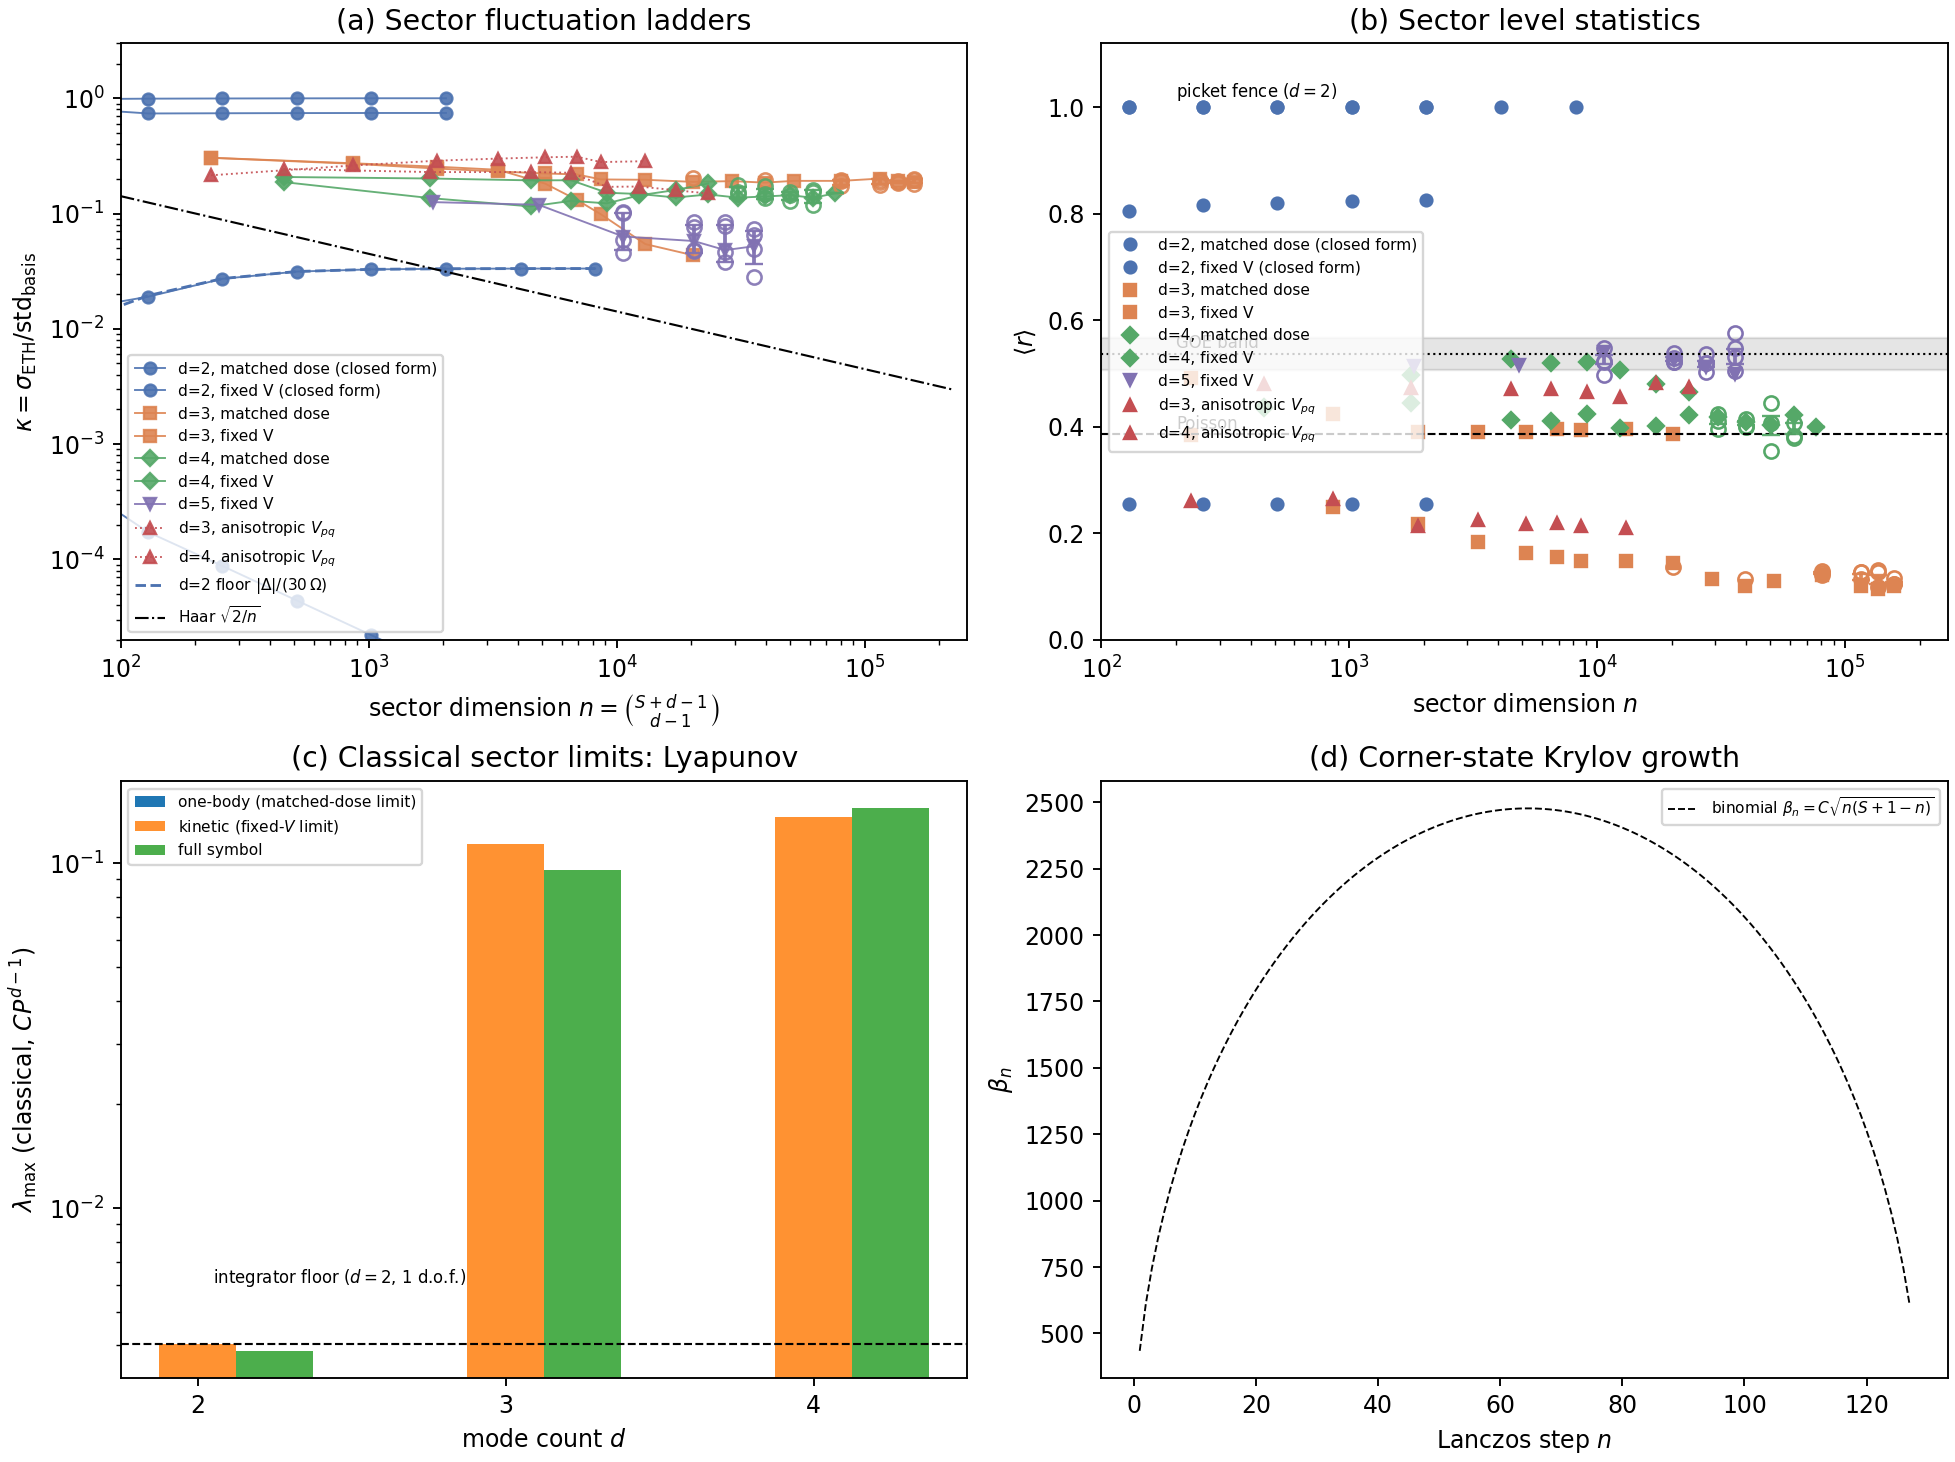
\includegraphics[width=\textwidth]{fig_c4_msector.png}
\caption{Occupation-sector falsifier ladders
(Remark~\ref{rem:numerics}(l)). (a)~The fluctuation ratio
$\kappa=\sigma_{\mathrm{ETH}}/\mathrm{std}_{\mathrm{basis}}$ of the
mode-$1$ occupation against the sector dimension
$n=\binom{S+d-1}{d-1}$: matched-dose and fixed-$V$ families at $d=2$
(closed form, with the analytic floor $|\Delta|/(30\Omega)$), $d=3$,
$d=4$, the $d=5$ fixed-$V$ family, and $\pm30\%$ anisotropic controls,
against the Haar benchmark $\sqrt{2/n}$ (filled points: the seed-$7$
ladders; open circles: replicate controls; error bars: realization
means with between-realization spread over the amendment tail rungs).
(b)~Level statistics
$\langle r\rangle$ against $n$ with the Poisson and GOE references and
the GOE band; the $d=2$ picket fence sits at $\langle r\rangle=1$ at
every scale. (c)~Benettin exponents of the classical sector limits on
$\mathbb{C}P^{d-1}$: the one-body (matched-dose) flow is integrable at
every $d$, the kinetic (fixed-$V$) flow is chaotic for $d\ge3$.
(d)~Corner-state Lanczos coefficients $\beta_n$; the $d=2$ sequence is
the binomial law exactly.}
\label{fig:msector}
\end{figure}

\begin{figure}[t]
\centering
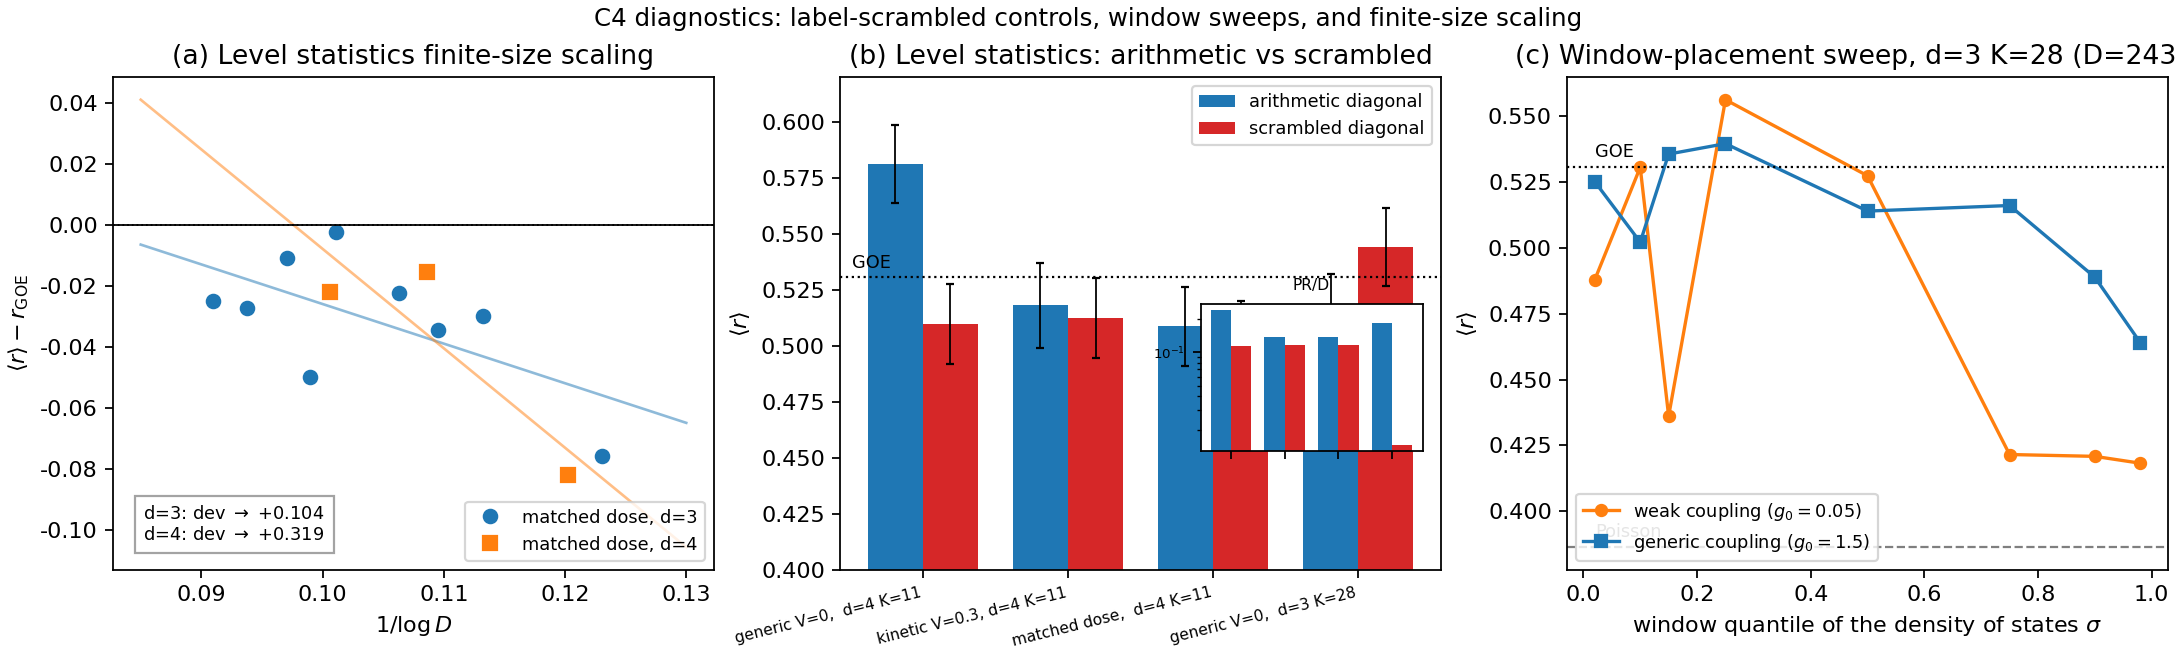
\includegraphics[width=\textwidth]{fig_c4_controls.png}
\caption{Audit-response controls for the $\mathsf{C4}$/$\mathsf{C5}$ numerics
(Remark~\ref{rem:numerics}(f)--(g)). (a)~Finite-size scaling of the level-statistics
deviation $\langle r\rangle-r_{\mathrm{GOE}}$ against $1/\log D$ along the matched-dose
ladders ($d=3$ circles, $d=4$ squares; fits as lines): deviations shrink with $D$ but the
computed range does not settle the limiting value. (b)~Arithmetic versus label-scrambled
diagonal at four platforms ($\langle r\rangle$ with standard errors; inset:
$\mathrm{PR}/D$ on a log scale): matched-dose $\langle r\rangle$ is
scramble-insensitive; the generic family is not, and the participation ratio collapses
under scrambling. (c)~Window-placement sweeps at $d=3$, $K=28$: the weak-coupling band
($0.42$--$0.56$) and the generic band ($0.46$--$0.54$) are both quantile-dependent; the
generic compression sits at the band edges.}
\label{fig:controls}
\end{figure}

\begin{figure}[t]
\centering
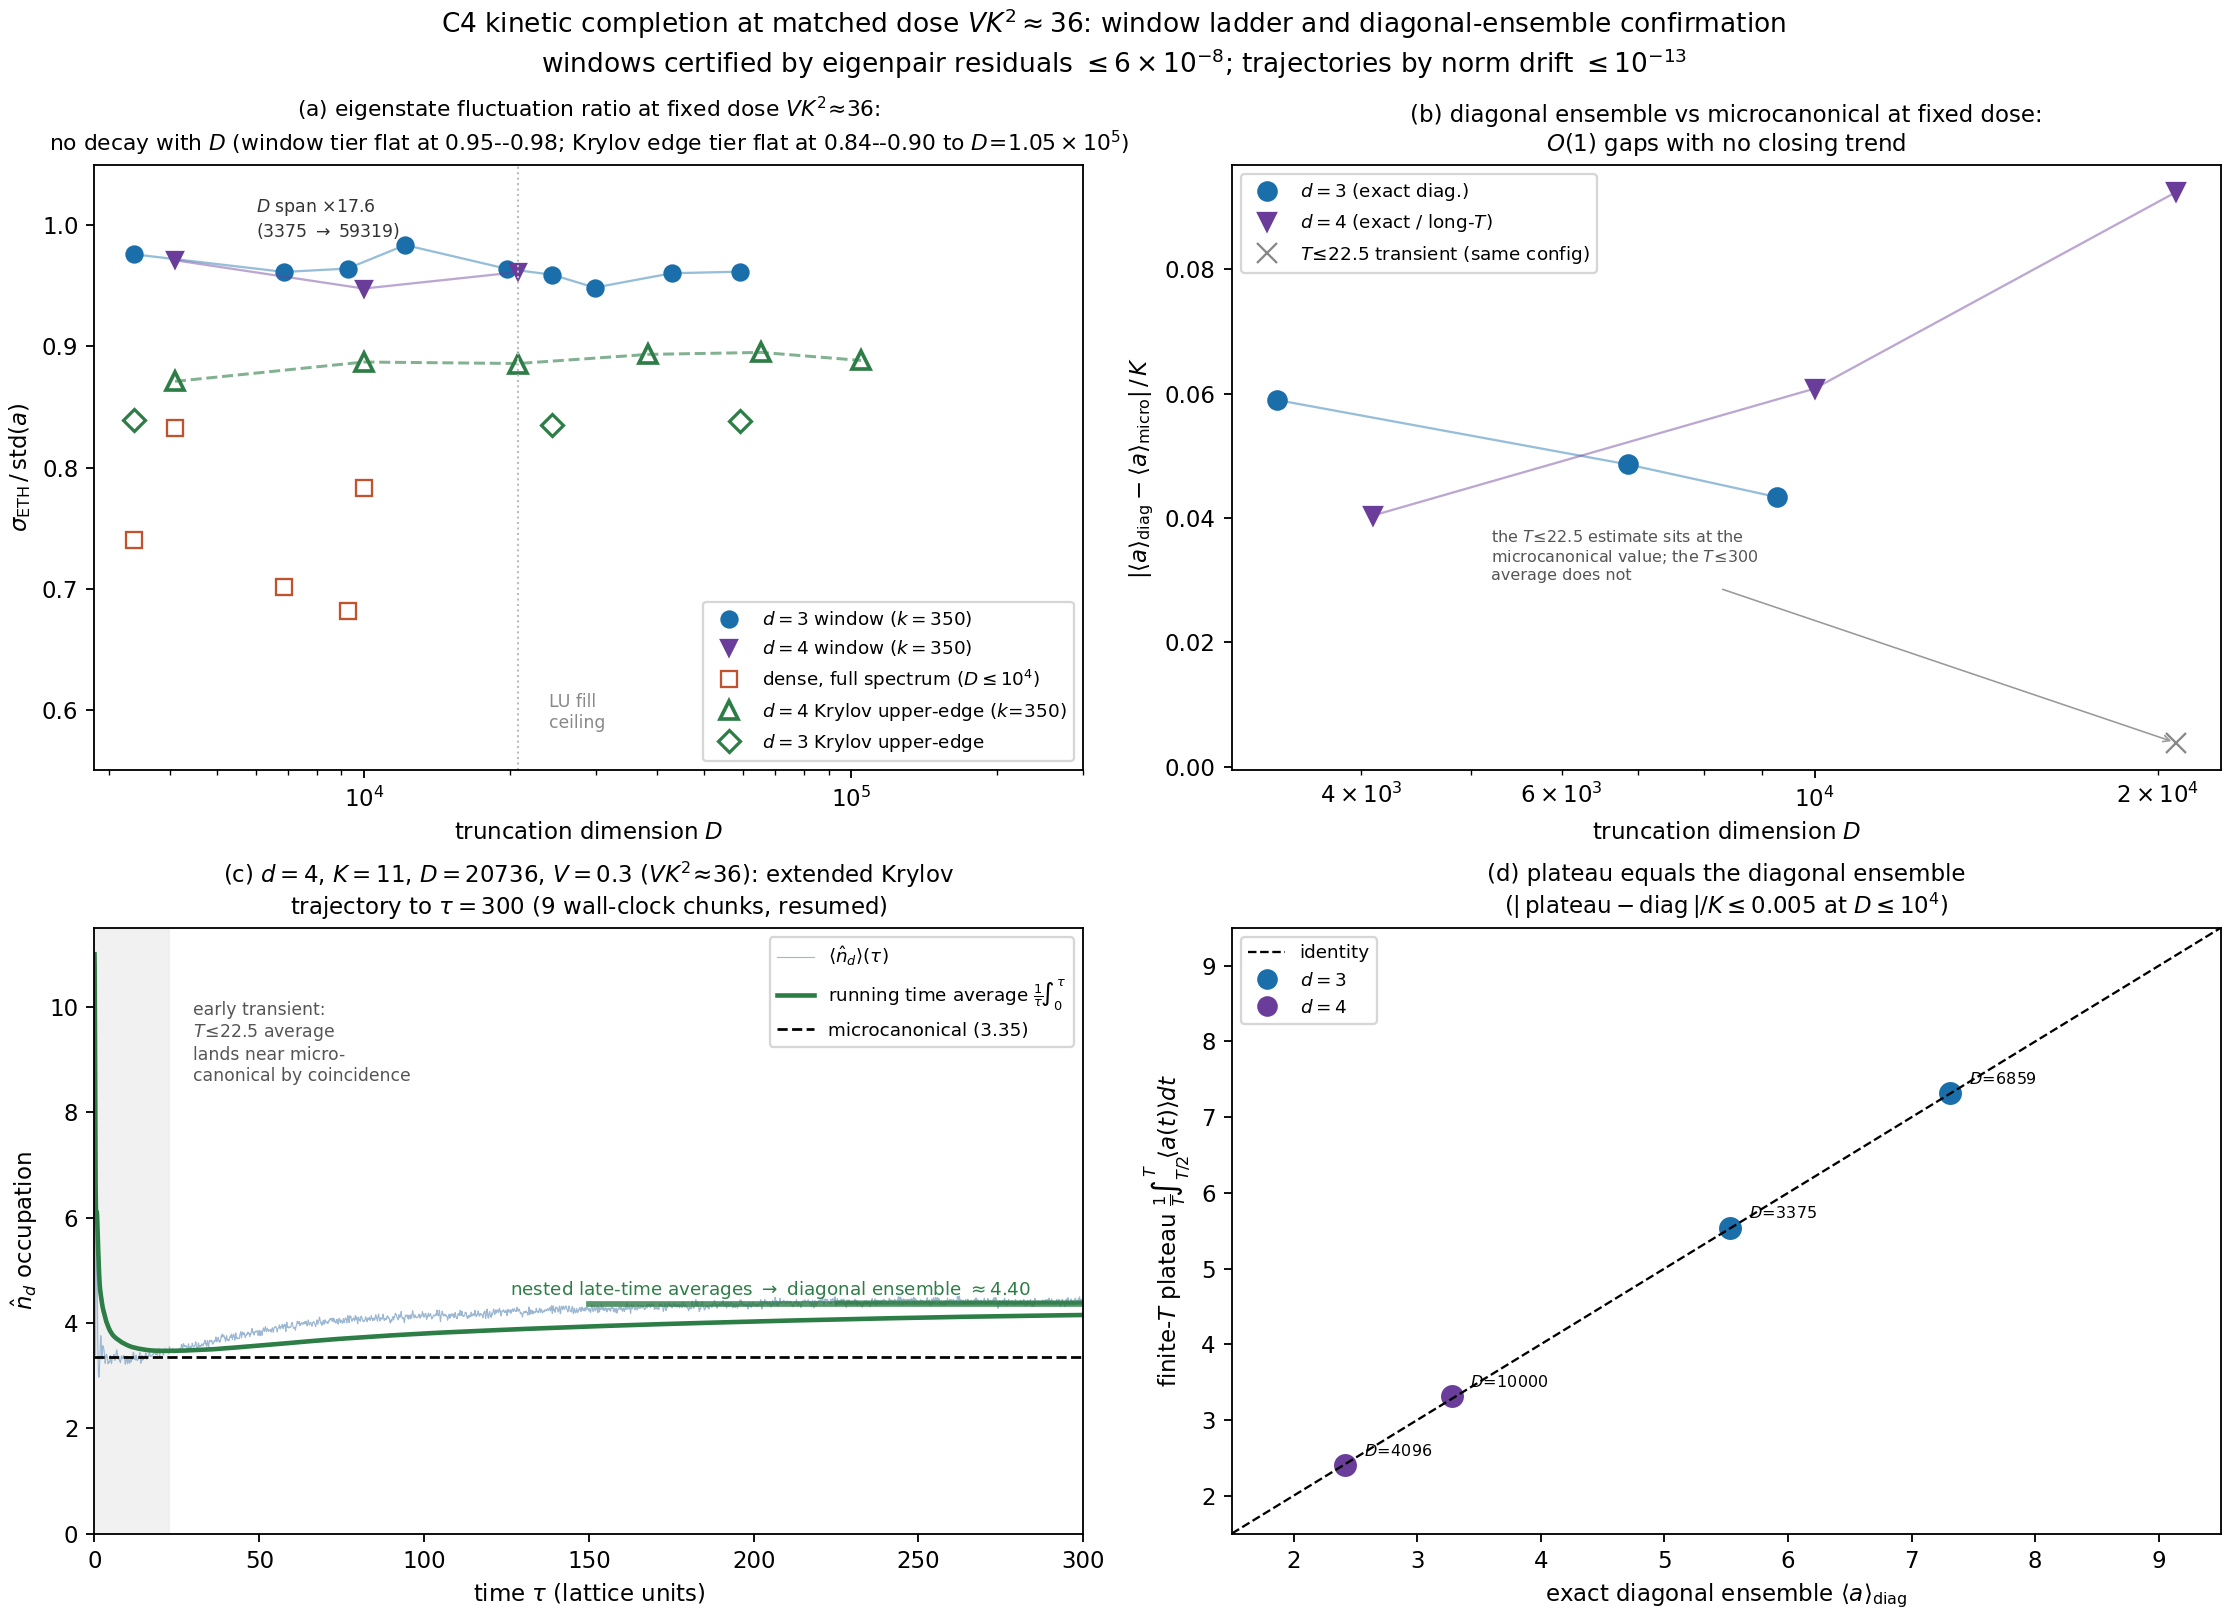
\includegraphics[width=\textwidth]{fig_c4_ladder.png}
\caption{Matched-dose ($VK^{2}\approx36$) numerics for the kinetic completion
(Remark~\ref{rem:numerics}(d)--(e)). (a)~Eigenstate fluctuation ratio
$\sigma_{\mathrm{ETH}}/\mathrm{std}(a)$ versus truncation dimension: window values
(filled) and exact full-spectrum values (open); no decay across a factor $17.6$ in $D$.
(b)~Distance of the diagonal ensemble from the microcanonical value, normalized by $K$:
$O(1)$ gaps with no closing trend; the $T\leq22.5$ estimate (cross) is a transient that
coincides with the microcanonical value. (c)~The $d=4$, $K=11$, $D=20736$, $V=0.3$
trajectory extended to $\tau=300$: observable, running time average, nested late-time
averages (diagonal-ensemble estimate $\approx4.40$), microcanonical line, and the early
transient. (d)~Finite-$T$ plateau versus exact diagonal ensemble at $D\leq10^{4}$ (identity
line).}
\label{fig:ladder}
\end{figure}

\begin{figure}[t]
\centering
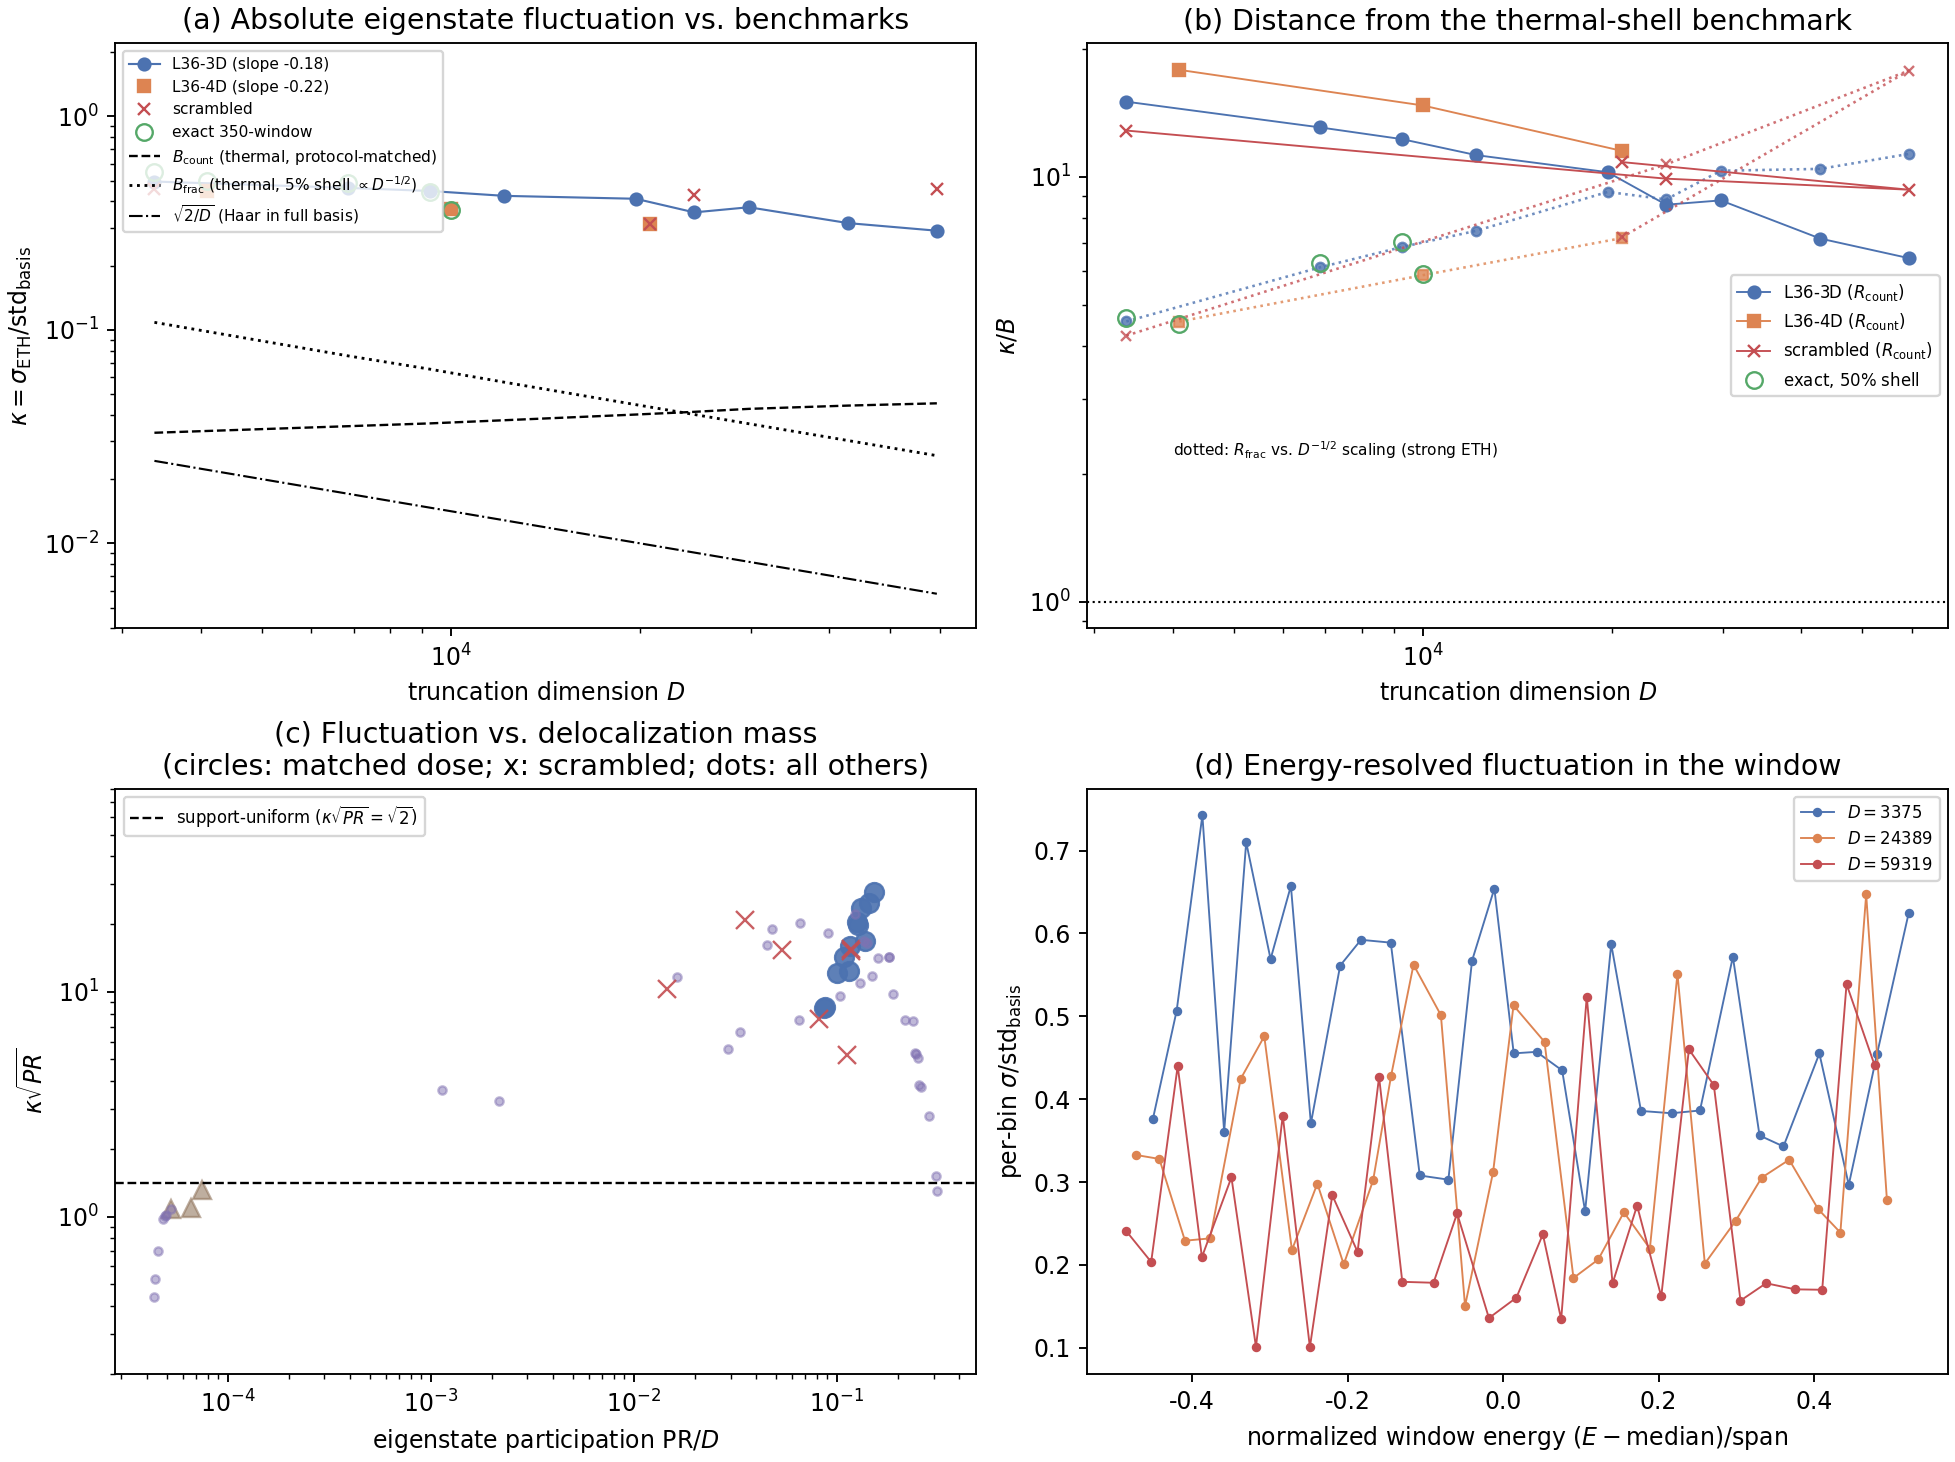
\includegraphics[width=\textwidth]{fig_c4_strongeth.png}
\caption{Absolute eigenstate-fluctuation scaling at matched dose
(Remark~\ref{rem:numerics}(h)--(i)).
(a)~$\kappa=\sigma_{\mathrm{ETH}}/\mathrm{std}_{\mathrm{basis}}$ versus truncation dimension
(window values, exact $350$-state selections, label-scrambled controls, and the
factorization-free Krylov-tier point at $D=3.84\times10^{4}$, open diamond: $276$ of
$350$ pairs certified) against the
calibrated benchmarks: the protocol-matched shell benchmark $B_{\mathrm{count}}$, the
fixed-fraction $B_{\mathrm{frac}}\propto D^{-1/2}$ (the strong-ETH scaling), and the
Haar-in-full-basis level $\sqrt{2/D}$. (b)~Distance from the benchmarks:
$\kappa/B_{\mathrm{count}}$ (solid) falls slowly; $\kappa/B_{\mathrm{frac}}$ (dotted) grows.
(c)~$\kappa\sqrt{\mathrm{PR}}$ versus eigenstate participation across all computed window
configurations (matched dose: circles; scrambled: crosses; all others: dots), against the
support-uniform level $\sqrt{2}$: the fluctuation sits $10$--$30$ times above it and grows
with $D$. (d)~Energy-resolved within-window fluctuation at three scales.}
\label{fig:strongeth}
\end{figure}

Falsifiers and test routes are listed in
Section~\ref{sec:register}.

\subsection{The Janus state}

A natural boundary condition is the vacuum: the claim that ``at the past hypothesis the
phase $1^{-i\omega_{0}\tau}=1$: time does not exist at $n=1$; time turns on when the universe
transitions to composite states.'' Under $H_{P}$ \emph{nothing} ever transitions
(Proposition~\ref{prop:frozen}), so the claim would be empty; under $H_{\mathrm{tot}}$ the vacuum
$\ket{1}$ is \emph{not} an eigenstate (because $H_{W}\ket{1}=\sum_{p}g_{p}\ket{p}$), and the
statement becomes substantive and true:

\begin{proposition}[Nucleation from the Janus state]\label{prop:nucleation}
For $H_{\mathrm{tot}}$ with $H_{W}\neq0$ and initial state $\psi(0)=\ket{1}$:
\begin{equation}
\psi(\tau)=\ket{1}-\frac{i\tau}{\hbar}\sum_{p\in P_{f}}g_{p}\ket{p}+O(\tau^{2}),
\end{equation}
so the \emph{total primon number} grows initially at rate
$d\langle\Nhat_{\mathrm{tot}}\rangle/d\tau=2\,\mathrm{Im}\,\langle\psi|H_{W}|\psi\rangle
/\hbar+O(\tau)=\frac{2\tau}{\hbar^{2}}\sum_{p}g_{p}^{2}+O(\tau^{2})>0$. The unique
zero-entropy state $\ket{1}$ is a regular point of the dynamics, not a fixed point; under
$H_{P}$ alone it is a fixed point (Proposition~\ref{prop:frozen}).
\end{proposition}

\begin{proof}
First-order time-dependent perturbation theory around the eigenstate $\ket{1}$ of $H_{P}$
(the Dyson series in $H_{W}+H_{\mathrm{hop}}$; $H_{\mathrm{hop}}$ annihilates the vacuum).
\end{proof}

Time, in this framework, is switched on by the interaction sector, with a mechanism that
exists. The stronger claims that
the actual history of the universe \emph{begins} at $\ket{1}$, and that the entropy profile is
two-sided (Janus-shaped) about that event, are boundary-condition statements and are demoted
to Conjectures $\mathsf{C7}$ and $\mathsf{C8}$; what remains as theorem is only the
uniqueness and zero entropy of the floor (Theorem~\ref{thm:spectrum} and
Section~\ref{sec:thermo}).

\section{Recurrence, Periodicity, and the Fate of Eternal Return}\label{sec:recurrence}

The anti-cyclical verdict---that prime arithmetic rigorously forbids exact cyclical
time and the universe cannot repeat---decomposes into a theorem, a correct application,
and two qualifications. This section separates them. The
resulting statement is \emph{stronger} than the slogan, because it identifies
exactly which recurrence phenomena are forbidden, which are unavoidable, and what the
boundary between them depends on.

\subsection{Linear independence of the prime logarithms}

\begin{lemma}[Fundamental-theorem independence]\label{lem:independence}
Every \emph{finite} $\Qq$-linear relation among the $\log p$ is trivial: the set
$\{\log p:p\in\Pr\}$ is $\Qq$-linearly independent in the finite-support sense. In
particular, for distinct primes
$p,q$, the ratio $\log p/\log q$ is irrational.
\end{lemma}

\begin{proof}
Suppose $\sum_{i=1}^{r}q_{i}\log p_{i}=0$ with $q_{i}=a_{i}/b_{i}\in\Qq$ and distinct primes
$p_{i}$. Let $B=\mathrm{lcm}(b_{i})$ and $c_{i}=Bq_{i}\in\Zz$. Then
$0=\sum_{i}c_{i}\log p_{i}=\log\prod_{i}p_{i}^{c_{i}}$ (negative exponents handled by clearing
signs into the other side), so $\prod_{i}p_{i}^{c_{i}}=1$. Unique factorization forces
$c_{i}=0$ for all $i$, hence $q_{i}=0$.
\end{proof}

\subsection{Exact periodicity is forbidden}

\begin{theorem}[No exact return for generic states]\label{thm:noperiod}
Let $\psi=\sum_{n}c_{n}\ket{n}$ and let $S(\psi)=\{n:c_{n}\neq0\}$ be its support. The
following are equivalent:
\begin{enumerate}[leftmargin=1.6em]
\item There exists $\tau>0$ with $e^{-i\tau H_{P}/\hbar}\psi=\psi$;
\item There exists $T>0$ such that $\omega_{0}T\log n\in2\pi\Zz$ for every $n\in S(\psi)$;
\item The set $\{\log n:n\in S(\psi)\}$ is contained in $\alpha\,\Zz$ for some $\alpha>0$
(all supports are integer multiples of a common logarithmic unit; equivalently all $n\in
S(\psi)$ are powers of a single integer).
\end{enumerate}
In particular, if $S(\psi)$ contains any two integers $m,n$ that are not powers of a common
integer---for example any pair among $\{2,3\}$, $\{6,10\}$, $\{2,6\}$---then $\psi$ is
aperiodic: $e^{-i\tau H_{P}/\hbar}\psi\neq\psi$ for every $\tau>0$. The same holds for
$H_{\mathrm{tot}}$ whenever its spectrum is simple and contains two levels whose difference is
irrational in units of $\hbar/\omega_{0}$, which holds generically.
\end{theorem}

\begin{proof}
$e^{-i\tau H_{P}/\hbar}\psi=\sum_{n}c_{n}e^{-i\omega_{0}\tau\log n}\ket{n}$ equals $\psi$ iff
$e^{-i\omega_{0}\tau\log n}=1$ for all $n\in S(\psi)$, i.e. iff
$\omega_{0}\tau\log n\in2\pi\Zz$ for all such $n$. Setting $\alpha=2\pi/(\omega_{0}\tau)$,
this says every $\log n$ in the support lies in $\alpha\Zz$. If $m,n\in S$ and
$\log m,\log n\in\alpha\Zz$ with $\log m/\log n\notin\Qq$, the condition fails for every
$\tau$; by Lemma~\ref{lem:independence}, $\log 2/\log 3\notin\Qq$ etc.
\end{proof}

This is the rigorous core of the anti-cyclic verdict: \emph{eternal return in the exact sense
requires the support of the universal state to lie in a single geometric progression of
integers}, and no physically motivated state does. The ray version (periodicity up to a global
phase, i.e.\ for physical states rather than vectors) relaxes the condition to: all ratios
$n/m$ with $n,m\in S(\psi)$ are powers of a single rational---the support lies in one
multiplicative coset $\{c\,a^{j}\}$. This too fails for any support with two
multiplicatively independent ratios (e.g.\ $S=\{6,12,18\}$: the ratios $2$ and $\tfrac32$
are independent by unique factorization), so the aperiodicity verdict is unchanged at the
level of rays.

\subsection{What is \emph{not} forbidden: three qualifications}

\begin{corollary}[Truncated systems recur]\label{cor:truncatedrecurrence}
Fix a finite truncation: primes $p\leq X$ and occupations $k_{p}\leq K$, so the Hilbert space
is finite-dimensional and the spectrum $\{E_{j}\}$ of $H_{P}$ (or of any self-adjoint
extension) is finite. Then the evolution $U(\tau)=e^{-i\tau H/\hbar}$ is a quasi-periodic
rotation, and for every state $\psi$ and every $\varepsilon>0$ the set
$\{\tau>0:\|U(\tau)\psi-\psi\|<\varepsilon\}$ is \emph{relatively dense} (there exists
$L=L(\varepsilon,\psi)$ such that every interval of length $L$ contains such a $\tau$). In
particular Poincar\'e recurrence holds in its strongest (uniform, Bohr almost-periodic) form.
This is the finite-dimensional special case of Theorem~\ref{cor:nopoincare} below, recorded
separately because it is the form in which recurrence appears in any \emph{computation}.
\end{corollary}

\begin{proof}
On a finite-dimensional space $U(\tau)=e^{-i\tau\Lambda}$ with
$\Lambda=\mathrm{diag}(E_{1},\dots,E_{d})/\hbar$; the map $\tau\mapsto
(e^{-i\tau E_{1}/\hbar},\dots,e^{-i\tau E_{d}/\hbar})$ is a continuous one-parameter
subgroup of the compact torus $\mathbb{T}^{d}$, and every orbit of a compact group rotation is
uniformly recurrent: the return times to any neighborhood of the identity are syndetic. This
is Kronecker's theorem in its group form \cite{hardywright2008}.
\end{proof}

\begin{theorem}[Uniform recurrence of the free flow, infinite system]\label{cor:nopoincare}
For \emph{every} state $\psi\in\Hil_{\mathcal{A}}$ and every $\varepsilon>0$, the set of
$\varepsilon$-return times
\begin{equation}
\Bigl\{\tau>0:\ \bigl\|e^{-i\tau H_{P}/\hbar}\psi-\psi\bigr\|<\varepsilon\Bigr\}
\end{equation}
is \emph{relatively dense} in $\Rr$. The free arithmetic flow is Bohr almost periodic for
all states, with no finite invariant measure required and no truncation assumed. What fails
is not $\varepsilon$-recurrence but its \emph{uniformity in the state}: the return-time
scale $L(\varepsilon,\psi)$ is unbounded as a function of $\psi$ (it grows with the
Diophantine complexity of the finite supports approximating $\psi$), and exact return
remains forbidden by Theorem~\ref{thm:noperiod}.
\end{theorem}

\begin{proof}
Fix $\varepsilon>0$ and $\psi=\sum_{n}c_{n}\ket{n}\in\ell^{2}$. Choose a finite support set
$F\subset\Nn_{\geq1}$ with $\sum_{n\notin F}|c_{n}|^{2}<\varepsilon^{2}/4$. The truncated
flow $\tau\mapsto\bigl(e^{-i\omega_{0}\tau\log n}\bigr)_{n\in F}$ is a continuous
one-parameter subgroup $h\colon\Rr\to\mathbb{T}^{F}$; let
$H=\overline{h(\Rr)}$, a compact connected subgroup of the torus. The $\Rr$-orbit of the
identity under left translation by $h(\tau)$ is dense in $H$ by construction, and a dense
orbit of an equicontinuous (group) action on a compact space is minimal; minimal
equicontinuous flows are uniformly recurrent, so
$T(\delta)=\{\tau:d(h(\tau),e_{H})<\delta\}$ is relatively dense for every $\delta>0$.
Taking $\delta$ small enough that all phases on $F$ deviate by less than $\varepsilon/2$
in the $\ell^{2}$ sense (finitely many constraints), we obtain
$\|U(\tau)\psi-\psi\|\leq\varepsilon/2+\varepsilon/2$ for every $\tau\in T(\delta)$, a
relatively dense set. The non-uniformity in $\psi$ follows because $F$ must grow as the
tails of $\psi$ shrink, and the Diophantine return times on $F$ are unbounded in $|F|$; the
quantitative form is Proposition~\ref{prop:returnbound} below.
\end{proof}

\begin{proposition}[Quantitative return-time bound]\label{prop:returnbound}
Let $\psi=\sum_{n}c_{n}\ket{n}$ be supported on a finite set $F\subset\Nn_{\geq1}$, let
$m_{F}=\#\{p: p\mid n \text{ for some } n\in F\}$ be the number of distinct prime
frequencies active in $F$, and let $K_{F}=\max_{n\in F}\max_{p}k_{p}(n)$. Then for every
$\varepsilon>0$ there exists an $\varepsilon$-return time
\begin{equation}\label{eq:returnbound}
\tau\;\leq\;\Bigl(\frac{2\pi C_{F}}{\varepsilon}\Bigr)^{m_{F}}
\qquad\text{with}\qquad C_{F}:=2+K_{F}m_{F},
\end{equation}
and the set of $\varepsilon$-return times is relatively dense with gaps of the same order
(Bohr's theorem \cite{besicovitch1932}).
\end{proposition}

\begin{proof}
Dirichlet's pigeonhole on the $m_{F}$-torus: with $N\geq2$, the $N^{m_{F}}+1$ points
$\{k\alpha\bmod 2\pi\}_{k=0}^{N^{m_{F}}}$, where
$\alpha=(\omega_{0}\log p)_{p\mid F}$, fall $N^{m_{F}}$-to-one into the $(2\pi/N)$-grid cells
of $\mathbb{T}^{m_{F}}$; two of them share a cell, and their difference $q\leq N^{m_{F}}$
satisfies $|q\,\omega_{0}\log p|_{\mathrm{mod}\ 2\pi}<2\pi/N$ for every $p\mid F$. Each phase of
$n\in F$ is the integer combination $\sum_{p}k_{p}(n)\,\omega_{0}\log p$ with
$\sum_{p}k_{p}(n)\leq K_{F}m_{F}$, so every phase on $F$ deviates by less than
$2\pi K_{F}m_{F}/N\leq\varepsilon$ once $N\geq2\pi K_{F}m_{F}/\varepsilon$ (choose also
$N\geq2$ so that the wrapped sum stays in $(-\pi,\pi]$). Then
$\|e^{-i\tau H_{P}/\hbar}\psi-\psi\|^{2}\leq\sum_{n}|c_{n}|^{2}|e^{i\theta_{n}}-1|^{2}
\leq\max_{n}|\theta_{n}|^{2}\leq\varepsilon^{2}$ with $\tau=q\leq N^{m_{F}}$. Relative
density with gaps of the same order is the syndeticity statement of Bohr almost-periodicity
\cite{besicovitch1932}.
\end{proof}

Proposition~\ref{prop:returnbound} is the quantitative content of ``Diophantine slowness'',
and it separates two recurrence scales that the framework needs kept apart.

\emph{Arithmetic} return. A typical integer near $x$ carries $\sim\log\log x$ distinct prime
factors (Theorem~\ref{thm:erdoskac}), so a superposition of $M$ integers near $x$ has
$m_{F}\lesssim M\log\log x$, and \eqref{eq:returnbound} gives
\begin{equation}\label{eq:arithreturn}
\tau_{\varepsilon}\;\lesssim\;(C/\varepsilon)^{M\log\log x}
\;=\;(\log x)^{M\log(C/\varepsilon)}
\;=\;(S/k_{B})^{O(1)},
\end{equation}
where $S(E)=k_{B}\log x=k_{B}E/\hbar\omega_{0}$ is the microcanonical entropy: for states
of fixed or slowly growing support, arithmetic $\varepsilon$-returns occur on times
\emph{polynomial in the entropy}. (The exponent $M\log(C/\varepsilon)$ is set by the support
size and the resolution; the occupations $K_{F}$ enter only the constant $C_{F}$, not the
exponent.)

\emph{Generic} return. A quantum system with $D$ resolved incommensurate frequencies
requires, by the same pigeonhole bound, $\tau_{\varepsilon}\gtrsim(\varepsilon^{-1})^{D}$. At
energy $E$ the arithmetic Hilbert space has $D=N(E)=e^{S/k_{B}}$ levels; a \emph{generic}
system on that many resolved frequencies needs
$\tau_{\varepsilon}\gtrsim e^{\,e^{S/k_{B}}\log(1/\varepsilon)}$: \emph{exponential in the
entropy} (doubly so). The primon gas occupies the extreme short-return end of this spectrum,
and the mechanism is exactly arithmetic: unique factorization compresses $D$ level
frequencies into the $m_{F}\ll D$ integer combinations of $\log p$.

For Conjecture $\mathsf{C2}$ this converts the qualitative cutoff language into a scaling
falsifier: recurrence phenomenology whose times grow faster than every power of the entropy
at fixed resolution $\varepsilon$ is inconsistent with every effective arithmetic cutoff
(upper bound \eqref{eq:arithreturn} changes only polynomially in $S$ when the cutoff $X$ or
$K$ is enlarged), while recurrence times polynomial in $S$ are the arithmetic prediction.
No cutoff-consistent adjustment absorbs an exponential-in-$S$ recurrence scale; conversely,
observed $\varepsilon$-returns at polynomial-in-$S$ times, for states of bounded support,
would be a signature of frequency compression of exactly the multiplicative kind.

The third qualification concerns the \emph{classical} multiplicative walk, and it sharpens
the boundary of the no-cycle verdict in an unexpected direction.

\begin{proposition}[P\'olya transience of the multiplicative walk]\label{prop:polya}
Consider the classical random walk on the divisibility graph of
Definition~\ref{def:multiplication} restricted to $d=|P_{f}|$ active primes: from
$k=(k_{1},\dots,k_{d})\in\Zz_{\geq0}^{d}$ step to $k+e_{j}$ with probability $1/(2d)$ and to
$k-e_{j}$ (when $k_{j}>0$) with probability $1/(2d)$, staying otherwise. Then the walk is
recurrent for $d\leq2$ and transient for $d\geq3$ \cite{polya1921}. In particular for
$d\geq3$ the walk returns to the vacuum $k=0$ (the Janus state) only finitely many times,
almost surely.
\end{proposition}

Proposition~\ref{prop:polya} has a striking interpretive reading: whether
the arithmetic universe ``cycles back to its origin'' depends on the \emph{number of active
prime modes}. With one or two primes, the multiplicative universe is recurrent---a rigorous
echo of cyclical cosmology. With three or more, it is transient, and the Janus point is a
genuinely singular origin. The absolute prohibition thus becomes a structural,
checkable dichotomy.

\subsection{The verdict on cyclical time}

Assembling the three legs: exact eternal return is impossible for states whose support spans
incommensurable integers (Theorem~\ref{thm:noperiod}); $\varepsilon$-approximate recurrence is
universal for the \emph{free} flow, at every state, with return times relatively dense but
astronomically non-uniform (Theorem~\ref{cor:nopoincare}, and
Corollary~\ref{cor:truncatedrecurrence} for the trivial finite case); and the \emph{cascading}
(or classical walk) dynamics is transient for $d\geq3$ modes (Proposition~\ref{prop:polya}),
with the interacting quantum system conjecturally non-recurrent on every physical scale
(Conjecture $\mathsf{C4}$). The philosophical consequences
are drawn in Section~\ref{sec:philosophy}; the essential point is that the framework's
anti-cyclical verdict survives as a \emph{layered} statement---exact return forbidden as a
genuine theorem, practical return driven out of reach by Diophantine slowness, transience
of the cascade for three or more active modes---rather than as an absolute metaphysical
prohibition. The free arithmetic sector, left to itself, is the \emph{most} recurrent object
in the theory (Bohr almost periodicity for all states, Theorem~\ref{cor:nopoincare}); all
irreversibility is therefore manufactured by the interaction sector and the boundary
condition, never by the spectrum. This is the sharpest available form of the intuition
that ``the river never circles back,'' and it is also the form most useful to
the arrow-of-time analysis of Sections~\ref{sec:time} and~\ref{sec:philosophy}.
% =====================================================================
% SECTION 5: The arithmetic clock  +  SECTION 6: Thermodynamics & gravity
% =====================================================================

\section{The Arithmetic Clock and the Problem of Time}\label{sec:time}

\subsection{The problem of time, stated precisely}

The reconciliation problem for the two classical concepts of time is standard: in
quantum mechanics, $t$ is an external parameter and the Schr{\"o}dinger equation evolves
states with respect to it; in general relativity, elapsed time is the proper time along a
worldline, $\tau_{\gamma}=c^{-1}\int_{\gamma}\sqrt{-g_{\mu\nu}dx^{\mu}dx^{\nu}}$, a geometric
quantity that varies from trajectory to trajectory, while the canonical Hamiltonian of
gravity is a constraint, $\Hmax\Psi=0$, with no external evolution at all. The
resolution is relational: time is a correlation between subsystems, realized quantum
mechanically by the Page--Wootters mechanism \cite{pagewootters1983}, with the primon
spectrum supplying the clock. This section turns that resolution into theorems, corrects
one sign-of-life issue (the clock kernel never decorrelates, so the arrow
of time cannot live in the clock), and quantifies the claim that ``at the
Janus point time does not exist.''

The Page--Wootters construction is standard: for a total state $\Psi$ satisfying a constraint
$(H_{C}+H_{S})\Psi=0$ of clock-plus-system, the conditional state of the system when the
clock reads $\tau$ is $\psi_{S}(\tau)=\bra{\tau}\Psi\rangle$, and for an ideal clock family
this satisfies an effective Schr{\"o}dinger equation in $\tau$. All content therefore
concentrates in the clock family. The analysis below supplies the \emph{kinematical} level of
this program: the clock family, the conditional-state map, and the correlation kernel. The
constraint equation itself is not solved here---solving it requires the interaction sector of
Section~\ref{sec:dynamics} and belongs to the content of $\mathsf{C4}$---and no claim is made
that this section dissolves the problem of time; what is proved is the exact correlation
structure of the arithmetic clock, and the exact statement of what that structure forbids.

\subsection{The zeta clock}

\begin{definition}[Zeta clock family]\label{def:clock}
For a dimensionless regulator $\nu>\tfrac12$ define the normalized clock states
\begin{equation}\label{eq:clockstates}
\ket{\tau;\nu}\;=\;\zeta(2\nu)^{-1/2}\sum_{n=1}^{\infty}n^{-\nu-i\omega_{0}\tau}\ket{n},
\end{equation}
a unit-norm family in $\Hil_{\mathcal{A}}$ (unit norm because $\sum_{n}n^{-2\nu}=\zeta(2\nu)$
converges for $2\nu>1$). The regulator is a resolution parameter, not a temperature: the
weights $n^{-\nu}$ confine the clock to energies of order
$\hbar\omega_{0}/(2\nu-1)$, as computed in Proposition~\ref{prop:uncertainty}. A clock at
regulator $\nu$ has the same mean energy as a canonical primon state at $\sigma=2\nu$; the
clock family therefore exists on \emph{both} sides of the Hagedorn scale---$\nu\downarrow\tfrac12$
is the high-energy (canonical-divergence) limit, $\nu\to\infty$ the vacuum limit---and it is
the analytic object through which energies above $T_{H}$, where no Gibbs state exists, are
nevertheless resolved (Section~\ref{sec:arithmetic}).
\end{definition}

\begin{proposition}[Clock covariance and two-time kernel]\label{prop:kernel}
\begin{enumerate}[leftmargin=1.6em]
\item (Covariance.) $e^{-i\tau' H_{P}/\hbar}\ket{\tau;\nu}=\ket{\tau+\tau';\nu}$: clock
translations are generated by $H_{P}$ itself, so the clock reading $\tau$ is exactly the
phase parameter conjugate to $\log\Nhat$,
\begin{equation}
e^{-i\omega_{0}\tau\log\Nhat}\ket{n}=n^{-i\omega_{0}\tau}\ket{n}.
\end{equation}
\item (Two-time kernel.) For all $\tau,\tau'$,
\begin{equation}\label{eq:kernel}
\braket{\tau';\nu}{\tau;\nu}
\;=\;\frac{\zeta\bigl(2\nu-i\omega_{0}(\tau-\tau')\bigr)}{\zeta(2\nu)}.
\end{equation}
\item (Positivity.) The kernel \eqref{eq:kernel} is positive definite on $\Rr$: it is the
Fourier transform of the probability measure
$\mu_{\nu}=\zeta(2\nu)^{-1}\sum_{n}n^{-2\nu}\delta_{\log n}$ on the energy-per-mode
variable $u=\log n$.
\item (Product of phases.) For a superposition $\sum_{n}c_{n}\ket{n}$ evolved for time
$\tau$, the phase acquired is $n^{-i\omega_{0}\tau}$, and by unique factorization
\begin{equation}
n^{-i\omega_{0}\tau}=\prod_{p}p^{-i\omega_{0}\tau\,k_{p}}:
\end{equation}
each prime contributes an elementary phase generator, and composite evolution is the product
of prime evolutions. This is the exact sense in which ``primes provide the elementary
generators of spectral phase order.''
\end{enumerate}
\end{proposition}

\begin{proof}
(1) is immediate term by term. (2) $\braket{\tau';\nu}{\tau;\nu}
=\zeta(2\nu)^{-1}\sum_{n}n^{-2\nu}e^{i\omega_{0}(\tau-\tau')\log n}
=\zeta(2\nu)^{-1}\zeta(2\nu-i\omega_{0}(\tau-\tau'))$, since
$e^{i\omega_{0}\Delta\tau\log n}=n^{i\omega_{0}\Delta\tau}$. (3) The kernel
$K(\Delta\tau)=\int e^{i\omega_{0}\Delta\tau u}\,d\mu_{\nu}(u)$ is the characteristic
function of $\mu_{\nu}$ composed with a dilation, hence positive definite by Bochner's
theorem. (4) follows from unique factorization applied to the logarithm of the phase.
\end{proof}

Equation~\eqref{eq:kernel} is the framework's signature formula: \emph{the
distinguishability of two readings of the arithmetic clock is governed by the Riemann zeta
function}. What follows adds
the facts that make it usable.

\begin{theorem}[Almost-periodicity of the clock: the arrow cannot live here]\label{thm:bohr}
For every $\nu>\tfrac12$, the kernel $K(\Delta\tau)=\zeta(2\nu-i\omega_{0}\Delta\tau)/\zeta(2\nu)$
is a Bohr almost-periodic function of $\Delta\tau$ \cite{besicovitch1932} (the Dirichlet series
converges absolutely on the line $\sigma=2\nu>1$). Consequently:
\begin{enumerate}[leftmargin=1.6em]
\item $|K|$ does \emph{not} decay along any sequence: $\limsup_{|\Delta\tau|\to\infty}|K(\Delta\tau)|=1$.
\item For every $\varepsilon>0$ the set
$\{\Delta\tau:|K(\Delta\tau)-1|<\varepsilon\}$ is relatively dense: clock correlations
resynchronize infinitely often, in both time directions, at every resolution $\nu$.
\end{enumerate}
No limit $\nu\downarrow\tfrac12$ escapes this: at every fixed $\nu$ the kernel is two-sided
symmetric, and the singular limit only narrows the correlation peak
(Proposition~\ref{prop:uncertainty}(2)) without ever selecting a direction. The high-energy
clock is \emph{more} resolved, not \emph{directed}.
\end{theorem}

\begin{proof}
On the line $\sigma=2\nu>1$, $\zeta(s)=\sum_{n}n^{-s}$ is an absolutely convergent Dirichlet
series with $\sum_{n}n^{-\sigma}<\infty$, hence a (uniform limit of finite exponential sums)
Bohr almost-periodic function of the imaginary part \cite{besicovitch1932}. Almost-periodic
functions have relatively dense $\varepsilon$-almost-periods, and $K(0)=1$.
\end{proof}

This theorem resolves a hidden tension in the framework. The zeta
object appears twice: as the clock (``the distinguishability of two times is
governed by the zeta function'') and as the engine of the thermodynamic arrow (``the
cascade up the mountain of composite numbers''). Theorem~\ref{thm:bohr} shows
these two roles cannot be fused: an almost-periodic clock is \emph{recurrent} and carries no
arrow. In the framework the arrow is therefore relocated entirely to the
interaction sector and the boundary condition (Conjecture $\mathsf{C4}$ and $\mathsf{C7}$),
while the clock contributes the neutral, arrow-free, maximally stable phase reference. This
is a structural clarification, not a loss: it says that \emph{within the framework, time
measurement and time's arrow are functionally separated objects}, exactly as relational
philosophy of time requires.

\subsection{Energy--time duality of the arithmetic clock}

\begin{proposition}[Resolution duality]\label{prop:uncertainty}
For the clock family $\ket{\tau;\nu}$:
\begin{enumerate}[leftmargin=1.6em]
\item The mean energy is
$\langle H_{P}\rangle_{\nu}=\hbar\omega_{0}\bigl(-\zeta'/\zeta\bigr)(2\nu)
=\dfrac{\hbar\omega_{0}}{2\nu-1}+O(\hbar\omega_{0})$ as $\nu\downarrow\tfrac12$.
\item The correlation peak is asymptotically Lorentzian: as $\nu\downarrow\tfrac12$,
uniformly for bounded $\omega_{0}\Delta\tau/(2\nu-1)$,
\begin{equation}
|K(\Delta\tau)|^{2}
=\frac{(2\nu-1)^{2}}{(2\nu-1)^{2}+\omega_{0}^{2}\Delta\tau^{2}}\,\bigl(1+o(1)\bigr),
\end{equation}
with half-width $\Delta\tau_{1/2}\asymp(2\nu-1)/\omega_{0}$.
\item Consequently $\langle H_{P}\rangle_{\nu}\,\Delta\tau_{1/2}\to\hbar$ as
$\nu\downarrow\tfrac12$: the zeta clock asymptotically saturates the
Mandelstam--Tamm energy--time limit. Time resolution is bought one-for-one with clock energy,
and the clock never becomes ``cheap.''
\item Conversely, as $\nu\to\infty$ the state concentrates on $\ket{1}$:
$\ket{\tau;\nu}\to\ket{1}$, energy $\to0$, and $K\to1$ for all $\Delta\tau$: the clock
resolves nothing. At the Janus limit the clock degenerates---the quantified form of the
claim that ``at $n=1$ time does not exist.''
\end{enumerate}
\end{proposition}

\begin{proof}
(1) is Theorem~\ref{thm:hagedorn} at $\sigma=2\nu\downarrow1$. Positivity of $\langle H_P\rangle$ requires $\nu>1/2$, consistent with Definition~\ref{def:clock}. (2) Near the pole,
$\zeta(\sigma-it)=(\sigma-1-it)^{-1}+O(1)$, so
$|K|^{2}=|\sigma-1|^{2}/((\sigma-1)^{2}+t^{2})+o(1)$ with $t=\omega_{0}\Delta\tau$ and
$\sigma-1=2\nu-1$. (3) Multiply (1) and (2). (4) $n^{-2\nu}$ concentrates on $n=1$;
$K(t)=\zeta(2\nu-it)/\zeta(2\nu)\to1$ since $\zeta(2\nu-it)\to1$ and
$\zeta(2\nu)\to1$.
\end{proof}

\subsection{Reconciliation of the three times}

With the clock machinery in place, the tripartite reconciliation can be stated as
a compact conditional statement. \emph{Quantum-mechanical time} is the reading of a
relational clock in the classical-clock limit: it is recovered when the clock subsystem is
large, weakly coupled, and quasi-classical, in which case $\tau_{\mathrm{clock}}\approx t$
for all practical observers. \emph{Relativistic time} is the proper-time functional along
worldlines: it is the geometric content of the clock's embedding, determining which phase
increments accumulate along which trajectory. \emph{Quantum-gravitational time} is the
constraint-generated phase correlation: with the primon clock, $\tau$ is conjugate to
$\log\Nhat$, and evolution is the multiplicative phase flow
$n^{-i\omega_{0}\tau}$. The three are not rivals but levels: the block-level correlation
structure ($\Hmax\Psi=0$), its geometric projection (proper time), and its semiclassical
limit (external $t$). All incompatibilities of principle dissolve at the kinematical level;
what remains open
is whether the \emph{specific} identification of the clock with the
primon spectrum is realized (Conjecture $\mathsf{C1}$), and how the geometric sector
emerges from the arithmetic one (Conjectures $\mathsf{C3}$, $\mathsf{C9}$).

The tripartite reconciliation is compactly stated:
\begin{center}
\emph{Relativity provides the geometry; quantum mechanics provides the spectrum; the primes
provide the arithmetic order of the spectrum; and time is the phase relation among
prime-ordered states measured along geometric worldlines.}
\end{center}
The measurement clause is Proposition~\ref{prop:kernel}(1) (clock covariance); the ordering
clause is unique factorization, i.e. Proposition~\ref{prop:kernel}(4); the arrow clause is
conspicuously absent, by Theorem~\ref{thm:bohr}, and lives in the interaction sector.

\section{Thermodynamics, Gravity, and the Holographic Bridge}\label{sec:thermo}

\subsection{The exact counting law}

A repeatedly used statement is ``the number of states below energy $E$ grows like
$e^{E/\hbar\omega_{0}}$.'' The exact statement is a one-line identity, and its precision is
what makes the holographic bridge in Section~\ref{sec:holography} clean.

\begin{theorem}[Log-count identity]\label{thm:logcount}
Let $N(E)=\#\{n\in\Nn_{\geq1}:\hbar\omega_{0}\log n\leq E\}=\lfloor e^{E/\hbar\omega_{0}}\rfloor$,
and write $x=E/\hbar\omega_{0}$ and $r(E)=\log N(E)-x$. Then:
\begin{enumerate}[leftmargin=1.6em]
\item (Global envelope.) For all $E\geq0$: $-\log2\leq r(E)\leq0$.
\item (Sharp two-sided bound, $E\geq\hbar\omega_{0}\log2$.)
\begin{equation}\label{eq:sharpdefect}
\log\bigl(1-e^{-x}\bigr)\;\leq\; r(E)\;\leq\; 0,
\end{equation}
with both bounds sharp: $r\uparrow0$ as $E$ crosses a level from above, and
$r\downarrow\log(1-e^{-x})$ as $E$ approaches a level from below.
\item (Exponential decay.) $|r(E)|\leq-\log(1-e^{-x})\leq 2e^{-x}$: the defect converges to
zero \emph{exponentially}. The counting function itself remains a staircase forever: $N$
jumps by one at every level $E=\hbar\omega_{0}\log m$, and the jump of $\log N$ there is
$\log\bigl(1+\tfrac1m\bigr)\sim\tfrac1m$---the granularity persists at every scale while its
amplitude decays like $e^{-x}$.
\item (Smoothing.) For every probability kernel $w$ supported in $[-\Delta,\Delta]$ with
$\Delta$ fixed, the smoothed count $\widetilde N=N\ast w$ satisfies, uniformly in
$E\geq\hbar\omega_{0}(\log2+\Delta)$,
\begin{equation}\label{eq:smoothing}
\log\widetilde N(E)\;=\;x\;+\;\log\!\int e^{t}w(t)\,dt\;+\;O(e^{-x}):
\end{equation}
the growth rate of every fixed-window smoothing of the entropy is exactly $1/\hbar\omega_{0}$
up to exponentially small corrections, at every energy scale.
\end{enumerate}
In particular the microcanonical entropy $S(E)=k_{B}\log N(E)$ satisfies
\begin{equation}
S(E)\;=\;\frac{E}{T_{H}}\;+\;\delta(E),
\qquad
|\delta(E)|\;\leq\;k_{B}\log\frac{1}{1-e^{-E/\hbar\omega_{0}}}\;\leq\;2k_{B}e^{-E/\hbar\omega_{0}}
\quad(E\geq\hbar\omega_{0}\log2),
\end{equation}
with $T_{H}=\hbar\omega_{0}/k_{B}$. (The unsmoothed entropy is a staircase; its pointwise
microcanonical temperature is undefined between levels. The content of the Hagedorn reading
is item~(iv): the growth rate is energy-independent, so energy input converts into state
multiplicity at a fixed exchange rate.)
\end{theorem}

\begin{proof}
$N(E)=\lfloor e^{x}\rfloor$ because $\hbar\omega_{0}\log n\leq E\iff n\leq e^{x}$. Write
$y=e^{x}$ and $\{y\}=y-\lfloor y\rfloor\in[0,1)$, so $r=\log\bigl(1-\{y\}/y\bigr)\in[\log(1-1/y),0]$
since $\lfloor y\rfloor\geq y-1$ and $\{y\}<1$. The lower bound is approached as $\{y\}\uparrow1$
($E$ approaching a level from below), the upper bound attained as $\{y\}\downarrow0$. Decay:
$-\log(1-u)\leq2u$ for $u\leq\tfrac12$, and $\{y\}/y<1/y=e^{-x}\leq\tfrac12$ for $x\geq\log2$.
Jumps: on $y\in[m,m+1)$, $\log N=\log m$ and the jump at $y=m+1$ is
$\log\bigl((m+1)/m\bigr)\sim1/m$. Smoothing: $N(E+t)=e^{x+t}-\{e^{x+t}\}$, so
$\widetilde N(E)=e^{x}\int e^{t}w(t)\,dt-R(E)$ with $0\leq R(E)=\int w(t)\{e^{x+t}\}\,dt\leq1$;
hence $\log\widetilde N=x+\log\int e^{t}w(t)dt+\log\bigl(1-R(E)e^{-x}/\!\int e^{t}w\bigr)$ and
the last term is $O(e^{-x})$, uniformly in $E$.
\end{proof}

Two consequences of the corrected defect estimate are load-bearing later, and both follow
from item~(iii). First, at matched entropy scale the integer-counting fluctuation is
$O(k_{B}e^{-E/\hbar\omega_{0}})$: \emph{far smaller} than the logarithmic corrections of
black-hole entropy, so those corrections cannot originate from the floor sector at
all---Section~\ref{sec:holography} turns this from a caveat into a falsifier (the counting
contributes no $\log A$ term; any such term must be carried by the dictionary). Second, the
fluctuation sector of the gravitational counting function is carried not by the floor but by
the \emph{prime}-counting oscillations: the explicit formula
$\psi(x)=x-\sum_{\rho}x^{\rho}/\rho+\cdots$ has fluctuations bounded by $O(\sqrt x\log^{2}x)$
under the Riemann hypothesis---the content of von Koch's equivalence
\cite{vonkoch1901}: the Riemann hypothesis is \emph{equivalent} to the statement that
arithmetic fluctuations about the smooth classical term are as small as
square-root-small. Read in the framework's dictionary, RH becomes: \emph{quantum
fluctuations of the arithmetic sector about the classical continuum are optimally
suppressed}. That is a rigorous reformulation of ``RH = spectral
stability'', and it is the strongest form of that claim that mathematics currently
licenses.

\subsection{The holographic bridge}\label{sec:holography}

The derivation of the Bekenstein--Hawking entropy from prime state counting
is a natural target. This paper isolates exactly one
nontrivial input and shows the rest is Theorem~\ref{thm:logcount}.

\begin{conjecture}[Arithmetic holographic bound]\label{conj:holobound}
The maximal primon excitation energy accessible in, or associated with, a spacetime region
whose boundary has area $A$ is
\begin{equation}\label{eq:holobound}
E_{\max}(A)\;=\;\frac{\hbar\omega_{0}}{4\ell_{P}^{2}}\,A\;+\;\hbar\omega_{0}\,s(A),
\qquad
s(A)=O\!\Bigl(\log\frac{A}{\ell_{P}^{2}}\Bigr),
\end{equation}
independently of the detailed matter content, where
$\ell_{P}=\sqrt{G\hbar/c^{3}}$ is the Planck length. The term $\hbar\omega_{0}s(A)$ is the
\emph{dictionary error term}: it is the only slot through which logarithmic corrections can
enter, since the counting theorem contributes none (Theorem~\ref{thm:logcount}(iii)).
\end{conjecture}

\begin{theorem}[Conditional Bekenstein--Hawking]\label{thm:bh}
Assume Conjecture~\ref{conj:holobound}. Then the arithmetic entropy of the region is
\begin{equation}
S(A)\;=\;k_{B}\log N\bigl(E_{\max}(A)\bigr)
\;=\;\frac{k_{B}A}{4\ell_{P}^{2}}\;+\;k_{B}\,s(A)\;+\;\delta\bigl(E_{\max}(A)\bigr),
\qquad
|\delta|\leq2k_{B}e^{-E_{\max}/\hbar\omega_{0}},
\end{equation}
which is the Bekenstein--Hawking entropy \cite{bekenstein1973,hawking1975} with the area
coefficient exact and \emph{every} logarithmic correction carried by the dictionary term
$s(A)$ and none by the counting. The pure model ($s=O(1)$) predicts no
$-\alpha\log(A/\ell_{P}^{2})$ term at all; a computed correction of that class (several
ensembles give $-\tfrac32\log A$) therefore falsifies the pure form and measures $s$.
Moreover, for a Schwarzschild black hole of
mass $M$, $A=16\pi G^{2}M^{2}/c^{4}$ and $A/4\ell_{P}^{2}=4\pi GM^{2}/(\hbar c)$; the choice
$E_{\max}=Mc^{2}$ and $\hbar\omega_{0}=2\,k_{B}T_{H}^{\mathrm{BH}}$ normalizes
\eqref{eq:holobound} \emph{exactly} at fixed horizon, with $T_{H}^{\mathrm{BH}}=\hbar c^{3}/(8\pi GMk_{B})$
the Hawking temperature.
\end{theorem}

\begin{proof}
Substitute \eqref{eq:holobound} into Theorem~\ref{thm:logcount}. For the Schwarzschild case,
$E_{\max}(A)/\hbar\omega_{0}=A/4\ell_{P}^{2}$ by \eqref{eq:holobound}; with
$E_{\max}=Mc^{2}$ this forces $\hbar\omega_{0}=4Mc^{2}\ell_{P}^{2}/A
=4Mc^{2}\cdot(G\hbar/c^{3})/(16\pi G^{2}M^{2}/c^{4})
=\hbar c^{3}/(4\pi GM)=2k_{B}T_{H}^{\mathrm{BH}}$.
\end{proof}

Two remarks delimit the bridge; both are registered under $\mathsf{C3}$.

\begin{remark}[The factor-of-two ambiguity]
The Hawking identification above is exact only per-horizon: since $T_{H}^{\mathrm{BH}}\propto
M^{-1}$, a \emph{universal} $\omega_{0}$ cannot equal $2T_{H}^{\mathrm{BH}}$ for all masses.
Either $\omega_{0}$ is universal and the identification holds to within
$O(1)$ horizon-dependent factors, or the arithmetic scale is set per horizon. Which
alternative survives is a genuine open question that the conjecture form makes explicit;
a presentation that silently treats $\omega_{0}$ as universal and the
identification as exact would hide it. In both alternatives the \emph{area coefficient} is
exact, because the counting defect is exponentially small (Theorem~\ref{thm:logcount}(iii));
all residual freedom lives in the dictionary term $s(A)$.
\end{remark}

\begin{remark}[What the bridge does and does not derive]
The bridge converts an area law into an \emph{energy} cutoff statement plus an exact
counting theorem; it does not derive the cutoff. This is precisely the logical position of
the holographic principle in mainstream theory, translated into arithmetic terms. The
conversion loss is provably zero in the area coefficient (Theorem
\ref{thm:logcount} has no hidden degeneracy factors, since the primon spectrum is simple,
Theorem~\ref{thm:spectrum}), and every logarithmic correction is imported through the
dictionary term $s(A)$: any slack in Conjecture~\ref{conj:holobound} is slack in the
physics, not in the counting.
\end{remark}

\subsection{Singularities and the Hagedorn wall}

The singularity claims swing between two poles: one places the primon gas
\emph{at} the singularity (the reported conformal system near the black-hole center), later
reading declares that singularities \emph{do not exist}. The reconciliation is a standard
move of effective field theory, and it is worth stating once, cleanly, because it removes
the apparent contradiction:

\begin{remark}[Resolution of the singularity tension]\label{rem:singularity}
``Singularity'' denotes the boundary of validity of the continuum effective description, not
a locus in the fundamental theory. In the reconstructed framework: the geometric (Einstein)
description fails where its implicit continuum counting diverges; the arithmetic description
remains finite at all energies (Theorem~\ref{thm:spectrum} has no finite accumulation
point, and all quantities are finite below $T_{H}$). The pole of $\zeta$ at $s=1$ is the
exact analytic signature of the breakdown: it is a \emph{critical} (Hagedorn) divergence,
not a curvature divergence. What the Big Bang and black-hole interiors ``are'' in this
framework is the regime where the geometric effective theory must be replaced by the
arithmetic one; the primon gas is the UV-complete description of \emph{that regime}, which is
compatible with it also being located, in the geometric coordinates of the effective theory,
``near the singularity.'' Both readings are thereby retained, each in its
proper tense. The associated physical conjecture ($\mathsf{C6}$) is that the Hagedorn wall
$T_{H}$ replaces the singular point: approach to the singularity is approach to a critical
temperature at which energy converts into primon creation rather than curvature growth.
\end{remark}

\subsection{Emergent gravity and the hierarchy problem}

The resolution of the hierarchy problem---gravity as an entropic, $1/N$-suppressed
collective effect \cite{jacobson1995,verlinde2011,thooft1974}---is the most speculative of
its physics claims, and it is demoted in full. But the demoted form can be made
unusually concrete, because the arithmetic sector supplies an explicit $N$.

\begin{conjecture}[Arithmetic hierarchy]\label{conj:hierarchy}
The Newton constant is set by the number of arithmetic degrees of freedom below the
effective cutoff $E_{\mathrm{cut}}$:
\begin{equation}
\frac{1}{G}\;\asymp\;\frac{\hbar}{c^{3}}\,\omega_{0}\,
N_{\mathrm{eff}}\bigl(E_{\mathrm{cut}}\bigr),
\qquad
N_{\mathrm{eff}}(E)=\lfloor e^{E/\hbar\omega_{0}}\rfloor,
\end{equation}
up to a dimensionless $O(1)$ factor, so that
\begin{equation}\label{eq:hierlog}
\log\frac{M_{\mathrm{Pl}}}{M_{\mathrm{EW}}}\;\asymp\;
\frac{E_{\mathrm{cut}}}{2\hbar\omega_{0}}
\qquad\Longrightarrow\qquad
E_{\mathrm{cut}}\;\asymp\;2\log\!\Bigl(\frac{M_{\mathrm{Pl}}}{M_{\mathrm{EW}}}\Bigr)\,\hbar\omega_{0}
\;\approx\;74\,\hbar\omega_{0}
\end{equation}
(using $M_{\mathrm{Pl}}/M_{\mathrm{EW}}\approx10^{16}$).
\end{conjecture}

The honest content of Conjecture~\ref{conj:hierarchy} is a \emph{relocation} of the hierarchy
problem, stated with numbers: the question ``why is gravity so weak?'' becomes ``why does the
effective arithmetic universe of the electroweak regime terminate at $n\sim e^{74}\approx
10^{32}$ integers?''---which is a question about the cutoff structure of the arithmetic
sector, not a fine-tuning of a Lagrangian parameter. The framework does not answer it; it
converts it into a well-posed question with a single dimensionless number to explain,
register entry $\mathsf{C11}$. This is strictly more than a bare
$1/N$-suppression narrative with no $N$, and strictly less than a derivation of $G$.

\subsection{The classical limit and the pole at unity}

The classical-limit condition reads: as $s\to1^{+}$, the coarse-grained
arithmetic partition function should reproduce classical geometry, the pole
$\zeta(s)\sim1/(s-1)$ representing the divergent continuum limit. This paper
restates this as a theorem-flanked analogy: the pole is exactly the Hagedorn divergence
(Theorem~\ref{thm:hagedorn}); the smooth term $x$ of $\psi(x)$ is the classical contribution
and the zeros contribute the fluctuations (von Koch's equivalence
\cite{vonkoch1901}); and ``renormalization removing the pole'' means passing to the
finite part of the Laurent expansion, whose constant term is Euler's constant $\gamma$---the
arithmetic framework's first finite counterterm. Whether the geometric sector (Einstein
dynamics, $G_{\mu\nu}+\Lambda g_{\mu\nu}=8\pi GT_{\mu\nu}$) can actually be \emph{derived} as
this coarse-graining is the deepest part of Conjecture $\mathsf{C1}$ and is not claimed.
% =====================================================================
% SECTION 7: Entanglement: arithmetic superpositions and holism
% =====================================================================

\section{Entanglement: Arithmetic Superpositions and Holism}\label{sec:entangle}

\subsection{Composite integers are product states}

The framework's informal layer identifies quantum entanglement with multiplicative
composition: ``a composite number is mathematically entangled: it cannot be described
independently of its prime factors''; ``entanglement is not non-local communication, it is
multiplicative inseparability''; ``a composite number like $n=p_{A}\cdot p_{B}$ is a single,
inseparable mathematical entity.'' As quantum theory this is false. The correction
relocates arithmetic entanglement to where it genuinely lives---superpositions across
prime-mode bipartitions---and preserves the arithmetic content as structure rather than as
a false identification.

\begin{theorem}[Product structure of the occupation basis]\label{prop:productstructure}
Let $P_{A},P_{B}\subset\Pr$ be disjoint with $P_{A}\cup P_{B}=\Pr$, and let
$\mathcal{F}_{A},\mathcal{F}_{B}$ be the submonoids of $\mathcal{F}$ supported on
$P_{A},P_{B}$. The monoid isomorphism $\mathcal{F}\cong\mathcal{F}_{A}\times\mathcal{F}_{B}$
(unique factorization: $k\mapsto(k|_{P_{A}},k|_{P_{B}})$) induces a unitary
\begin{equation}
\Hil_{\mathcal{A}}\;\cong\;\Hil_{A}\otimes\Hil_{B},
\qquad
\ket{k}\;\mapsto\;\ket{k_{A}}\otimes\ket{k_{B}},
\end{equation}
under which every occupation basis vector is a \emph{product state}. In particular
$\ket{pq}=\ket{p}_{A}\otimes\ket{q}_{B}$ for $p\in P_{A}$, $q\in P_{B}$: a composite integer
is an \emph{unentangled} configuration of its prime factors. Entanglement across the
bipartition is a property of \emph{superpositions}
$\psi=\sum c_{ij}\ket{i}_{A}\ket{j}_{B}$ of rank $>1$ in the coefficient tensor, exactly as
in ordinary quantum mechanics, and of nothing else.
\end{theorem}

\begin{proof}
The restriction map is a bijection of free commutative monoids by unique factorization; the
induced map on $\ell^{2}$ bases is a bijection of orthonormal bases preserving inner
products; extend linearly. Product structure of each basis vector is the definition of the
tensor identification.
\end{proof}

The composite-as-entangled picture thus becomes a precise dichotomy: the
integer $n$ \emph{labels} a product configuration; \emph{arithmetic entanglement} is
superpositional. The dichotomy is stronger than the identification it replaces, because it
carries
quantitative content: entanglement entropies, Schmidt ranks, and Bell
inequalities.

\begin{definition}[Arithmetic entanglement]\label{def:arithmeticent}
For a bipartition $\Pr=P_{A}\sqcup P_{B}$ and a pure state
$\psi\in\Hil_{A}\otimes\Hil_{B}$, the \emph{arithmetic entanglement entropy}
$S_{\mathrm{ent}}(\psi)$ is the von Neumann entropy of
$\rho_{A}=\Tr_{B}\ket{\psi}\bra{\psi}$. $\psi$ is entangled iff
$S_{\mathrm{ent}}(\psi)>0$, iff the coefficient tensor
$(c_{ij})$ in the occupation basis has rank $>1$ when reshaped as a matrix.
\end{definition}

\begin{example}[The six--thirty-six Bell pair]\label{ex:bellpair}
Take $P_{A}=\{2\}$, $P_{B}=\{3\}$. Then
\begin{equation}
\frac{1}{\sqrt2}\bigl(\ket{6}+\ket{36}\bigr)
=\frac{1}{\sqrt2}\bigl(\ket{2}_{A}\ket{3}_{B}+\ket{4}_{A}\ket{9}_{B}\bigr)
\end{equation}
is maximally entangled across the bipartition: Schmidt rank $2$, equal Schmidt values
$1/\sqrt2$, $S_{\mathrm{ent}}=\log2$. The superposition of the integers $6$ and $36$ \emph{is}
an arithmetic Bell pair. More generally
$\frac{1}{\sqrt2}(\ket{ab}+\ket{cd})$ with $a,c$ powers of distinct primes of $P_{A}$ and
$b,d$ of $P_{B}$, $(a,b)\neq(c,d)$, is maximally entangled.
\end{example}

\begin{proposition}[Bell violation in the arithmetic sector]\label{prop:chsh}
Restrict local measurements to the two-dimensional subspaces
$V_{A}=\mathrm{span}\{\ket{2},\ket{4}\}\cong\Cc^{2}$ and
$V_{B}=\mathrm{span}\{\ket{3},\ket{9}\}\cong\Cc^{2}$, identified with qubits. On the Bell
state of Example~\ref{ex:bellpair}, the standard spin settings along the $xz$-plane achieve
the CHSH value $2\sqrt2$, the Tsirelson bound \cite{chsh1969,bell1964}. Hence the arithmetic
sector, equipped with superpositional states, exhibits exactly standard quantum
non-locality of correlations; the violation is destroyed if the superposition is replaced by
either basis vector, i.e. by any definite integer.
\end{proposition}

\begin{proof}
The restriction of the state to $V_{A}\otimes V_{B}$ is the standard Bell state
$(\ket{00}+\ket{11})/\sqrt2$; the CHSH computation is the textbook one.
\end{proof}

\subsection{Splitting primes as natural entanglement resources}

The Gaussian sector supplies a construction the rational sector lacks, and it realizes two
images at once (the ``complex primon overlay'' of the five-dimensional
picture and the claim that symmetry breaking is prime splitting).

\begin{proposition}[Splitting-prime EPR pairs]\label{prop:splitting}
Let $p\equiv1\ (\mathrm{mod}\ 4)$ be a rational prime, so that
$p=\pi\bar\pi=N(\pi)$ in $\Zz[i]$ with $\pi$ a Gaussian prime, $\pi\sim\bar\pi$ conjugate and
non-associate. Define the \emph{splitting state}
\begin{equation}
\ket{p}_{\mathrm{split}}
\;=\;\frac{1}{\sqrt2}\Bigl(\ket{\pi}\otimes\ket{\bar\pi}
+\ket{\bar\pi}\otimes\ket{\pi}\Bigr)
\end{equation}
on the two Gaussian modes generated by $\pi$ and $\bar\pi$. Then:
\begin{enumerate}[leftmargin=1.6em]
\item $\ket{p}_{\mathrm{split}}$ is maximally entangled across the
$(\pi,\bar\pi)$ bipartition ($S_{\mathrm{ent}}=\log2$);
\item it is invariant under the conjugation involution $C$ (which swaps the two tensor
factors), so it is even under the arithmetic charge conjugation of
Section~\ref{sec:galois};
\item it is the natural correlate, inside the arithmetic Hilbert space, of the splitting of
$p$ in $\Zz[i]$---the phenomenon whose statistical frequency is exactly $1/2$ by
Chebotarev/Dirichlet (Section~\ref{sec:galois}).
\end{enumerate}
\end{proposition}

\begin{proof}
(1) The two tensor factors are qubit-spaces $\mathrm{span}\{\ket{\pi},\ket{\bar\pi}\}$; the
state is the symmetric Bell state. (2) $C$ exchanges $\ket{\pi}\leftrightarrow
\ket{\bar\pi}$ in each factor, and the state is manifestly symmetric. (3) The correspondence
$p\mapsto\{\pi,\bar\pi\}$ is the Dedekind--Kummer splitting theorem for $\Zz[i]$
\cite{neukirch1999}.
\end{proof}

Proposition~\ref{prop:splitting} is the precise version of the ``phantom layer of
Gaussian primes weaving through the solid prime nodes''; the weaving is entanglement between
conjugate prime modes, quantitatively $\log2$ per split integer, and it exists only for the
splitting class $p\equiv1\ (4)$, which by Dirichlet's theorem has natural density $1/2$. The
inert class $p\equiv3\ (4)$ contributes \emph{no} entanglement resource: those primes remain
prime in $\Zz[i]$. The arithmetic sector thus possesses an intrinsic, algebraically defined
binary---split versus inert---with exact statistics. Section~\ref{sec:galois} builds the
force-sector dictionary on it; it is also the natural habitat for the idea that the
weak (chiral) interaction lives in the complex sector.

\subsection{Measurement, decoherence, and records}

With entanglement defined correctly, the measurement picture---``a measurement is an
interaction that creates a thermodynamically irreversible, decohered record in the prime
spectrum''---translates into standard quantum mechanics with an arithmetic
state space, and the standard strengths \emph{and} standard weaknesses apply.

\begin{remark}[Measurement as record formation]
In this framework a measurement is an interaction between a system and a
macroscopic apparatus/environment whose net effect is to entangle the system's
superposition across the bipartition ``apparatus modes versus system modes'' so strongly
that the reduced state of the system is, to observational accuracy, diagonal in the
pointer basis (einselection) \cite{zurek2003}. The arrow enters through the thermodynamic
cost of stabilization (Landauer's principle \cite{landauer1961}): records can be written
reliably only in the direction of increasing multiplicity of environmental states, i.e. along
the cascade of Conjecture $\mathsf{C4}$. Rocks measure rocks, photons measure dust grains,
and consciousness is a consumer of records, not a precondition for them---each clause
survives, now attached to the correct mechanism (superposition
entanglement, Theorem~\ref{prop:productstructure}) rather than the incorrect one
(composite inseparability).
\end{remark}

\begin{remark}[The improper-mixture problem]
Decoherence diagonalizes reduced density matrices; it does not, by itself, select one
outcome. The framework elects an Everettian resolution
\cite{wallace2012}, registered as interpretive
(Conjecture $\mathsf{C12}$) rather than theorem-grade. What the arithmetic sector adds is
structural, not probabilistic: branching in $\Hil_{\mathcal{A}}$ is branching of
\emph{factorization histories}---worldlines through the divisibility graph---and the
Born-rule weights are the squared amplitudes of superposed integers. The 2019 reversal
experiments on small qubit registers \cite{lesovik2019} are consistent with this picture in
the same sense as with standard decoherence: small closed systems can be
complex-conjugated back; macroscopic entangled cascades cannot, because the required
inverse unitary acts on $\sim10^{80}$ correlated modes and its probability is beyond every
Poincar\'e time. The experiments were performed by Lesovik et al.\ and implemented on an IBM
quantum computer.
\end{remark}

\subsection{Bell's trilemma and the rejection of superdeterminism}

Superdeterminism can be rejected with the argument that Bell correlations arise from
``multiplicative inseparability'' of composites. That mechanism is false
(Theorem~\ref{prop:productstructure}), so the rejection must rest on other grounds: the standard
Everettian one, plus the arithmetic sector's own contribution:

\begin{enumerate}[leftmargin=1.6em]
\item \emph{Realism, global not local.} The arithmetic Hilbert space and the universal
state are observer-independent; individual prime modes carry no pre-existing local values
(the occupation basis is a basis, not a value assignment). This is exactly the
quantum theory's own position: realism preserved globally, rejected locally.
\item \emph{Locality, no-signaling not local action.} Arithmetic-entangled states
(Examples~\ref{ex:bellpair}, Proposition~\ref{prop:splitting}) exhibit Bell correlations
across spacelike separation (Proposition~\ref{prop:chsh}) while the reduced states are
untouched by distant operations: $\rho_{B}=\Tr_{A}\rho_{AB}$ is invariant under local
unitaries on $A$. No usable signal, energy, or conserved quantity propagates
superluminally; the no-signaling theorem is a theorem of the tensor structure that
Theorem~\ref{prop:productstructure} now correctly exhibits.
\item \emph{Statistical independence, preserved.} Measurement settings and hidden variables
are not pre-correlated by a cosmic conspiracy. The correlations of the Bell state are
\emph{created} by the state's preparation (a superposition), not imposed on separate
local beables. Superdeterminism saves locality only by denying independence; the arithmetic
framework keeps independence and gives up local realism of modes, exactly as
loophole-free experiments \cite{hensen2015} force \cite{bell1964,chsh1969}.
\end{enumerate}

The corrected position is the standard one, reached with the arithmetic sector's own
structure. The philosophical residue---that ``space'' itself is emergent from entanglement
structure, so that demands for local causal explanation between entangled modes are a
category error---remains available as an interpretation (register $\mathsf{C12}$), in the
same epistemic tier as the ER$=$EPR-type conjectures it echoes. What is theorem-grade is
narrower and cleaner: in the arithmetic sector, \emph{non-locality of correlations is a
property of superposed integers, local realism of prime modes is false, and no-signaling is
exact}.
% =====================================================================
% SECTION 8: The arithmetic gauge sector
% =====================================================================

\section{The Arithmetic Gauge Sector}\label{sec:galois}

\subsection{From Lie unification to Galois unification}

The framework proposes that the Standard Model gauge group
$\mathrm{U}(1)\times\mathrm{SU}(2)\times\mathrm{SU}(3)$ is the ``macroscopic, continuous
shadow'' of the Absolute Galois group $G_{\Qq}=\Gal(\bar\Qq/\Qq)$, with the Langlands
program as the dictionary, prime splitting as symmetry breaking, and Gaussian primes as the
chiral (weak) sector. As physics this is speculation; as mathematics it can be anchored on
all fours, because each ingredient of the analogy corresponds to an actual theorem. This
section therefore proceeds in two layers: a \emph{theorem layer} that fixes what is
true about splitting statistics and symmetry structure, and a \emph{dictionary layer} that
is demoted in its entirety (Conjecture $\mathsf{C9}$).

The theorem layer rests on three classical results, which we state in the form the analogy
uses them.

\begin{theorem}[Kronecker--Weber]\label{thm:kw}
Every finite abelian extension $K/\Qq$ is contained in a cyclotomic field
$\Qq(\zeta_{m})$; conversely every cyclotomic field is abelian over $\Qq$
\cite{neukirch1999}. Combined with Dirichlet's theorem on primes in arithmetic
progressions \cite{dirichlet1837} and the splitting criterion
\begin{equation}\label{eq:splittingcriterion}
p\nmid m,\ p\ \text{splits completely in}\ \Qq(\zeta_{m})
\iff p\equiv1\ (\mathrm{mod}\ m),
\end{equation}
the abelian sector of $G_{\Qq}$ is completely described by residue classes of primes: the
reciprocity map of class field theory is, explicitly, $p\mapsto p\ (\mathrm{mod}\ m)$.
\end{theorem}

\begin{theorem}[Dedekind--Kummer splitting]\label{thm:kummer}
Let $K=\Qq(\theta)$ with $\theta$ an algebraic integer of minimal polynomial $f$, and $p$ a
rational prime not dividing the index $[\mathcal{O}_{K}:\Zz[\theta]]$. Then the factorization
pattern of $f$ modulo $p$ into irreducibles of degrees $d_{1},\dots,d_{r}$ coincides with
the splitting pattern of $p$ in $\mathcal{O}_{K}$: $p\mathcal{O}_{K}
=\mathfrak{p}_{1}\cdots\mathfrak{p}_{r}$ with residue degrees $d_{1},\dots,d_{r}$
\cite{neukirch1999}. Symmetry breaking and prime splitting are the same operation.
\end{theorem}

\begin{theorem}[Chebotarev density]\label{thm:chebotarev}
Let $K/\Qq$ be a finite Galois extension with group $G$, and $\sigma\in G$ any element. The
set of rational primes $p$ (unramified in $K$) whose Frobenius class
$\Frob_{p}\subset G$ equals the conjugacy class of $\sigma$ has natural density
$|\mathrm{cl}(\sigma)|/|G|$ \cite{chebotarev1926}. In particular: splitting statistics are
group statistics. Dirichlet's theorem is the abelian case (with
Theorem~\ref{thm:kw}).
\end{theorem}

For the working example that carries the whole source dictionary, specialize to
$K=\Qq(i)$, $G=\Gal(\Qq(i)/\Qq)=\{1,\sigma\}$ with $\sigma$ the complex conjugation
$a+bi\mapsto a-bi$:

\begin{center}
\begin{tabular}{@{}llll@{}}
\toprule
Class of $p$ & Condition & Behavior in $\Zz[i]$ & Density (Chebotarev)\\
\midrule
Split & $p\equiv1\ (4)$ & $p=\pi\bar\pi$, two conjugate primes & $1/2$\\
Inert & $p\equiv3\ (4)$ & $p$ remains prime & $1/2$\\
Ramified & $p=2$ & $2=-i(1+i)^{2}$, one prime squared & $0$ (finite)\\
\bottomrule
\end{tabular}
\end{center}

\subsection{The dictionary}

With the theorem layer fixed, the force-to-field dictionary can be stated so that
every arithmetic entry is backed and every physical equation is demoted:

\begin{center}
\begin{tabular}{@{}p{0.30\textwidth}p{0.34\textwidth}p{0.30\textwidth}@{}}
\toprule
Standard Model object & Arithmetic object & Status of the pairing\\
\midrule
$\mathrm{U}(1)$ gauge structure &
Abelian extensions, cyclotomic fields $\Qq(\zeta_{m})$; the ``photon'' is the reciprocity
map $p\mapsto p\ (\mathrm{mod}\ m)$ &
Theorem layer: KW, Dirichlet (Thm~\ref{thm:kw}); pairing demoted ($\mathsf{C9}$)\\
Chiral $\mathrm{SU}(2)_{L}$, parity violation &
Quadratic/non-abelian extensions; the non-trivial automorphism $\sigma$ (conjugation) acts
as the arithmetic $C$; split/inert dichotomy as handedness &
Theorem layer: splitting table above; pairing demoted ($\mathsf{C9}$, $\mathsf{C10}$)\\
$\mathrm{SU}(3)$ color, confinement &
Inert primes ($p\equiv3\ (4)$ and their non-abelian analogues); higher-degree splitting
patterns with non-commuting Frobenius classes &
Theorem layer: Chebotarev (Thm~\ref{thm:chebotarev}); pairing demoted ($\mathsf{C9}$)\\
Higgs mechanism, spontaneous symmetry breaking &
Ramification and splitting: the unified base $\Qq$ extends to $K$; primes then
\emph{choose} splitting patterns, with exact group-valued statistics &
Theorem layer: Kummer (Thm~\ref{thm:kummer}); pairing demoted ($\mathsf{C9}$)\\
Coupling unification, charge quantization &
Langlands functoriality: transfer of automorphic representations between $L$-groups;
the dictionary itself &
Mathematics: deep conjecture, proven for $\mathrm{GL}_{n}$ over function fields
\cite{lafforgue2002}; physics: demoted ($\mathsf{C9}$)\\
CP violation, CKM phase &
The $\sigma$-odd interaction sector: asymmetric couplings
$w(\pi)\neq w(\bar\pi)$; the non-vanishing $L(1,\chi_{-4})=\pi/4$ as the arithmetic
asymmetry functional &
Theorem layer: factorization \eqref{eq:factorization}; model demoted ($\mathsf{C10}$)\\
\bottomrule
\end{tabular}
\end{center}

Each row now has the same structure: a true theorem about number fields, an honest
conjecture about the pairing. The table is a bookkeeping of identifications, not a
construction: no row supplies a gauge field, a connection, an action, a mass gap, or any
confinement or scattering observable, and none is derived anywhere in this section. Each
row's physical content is exactly its conjectural statistics---restrictions, densities,
hierarchies---and nothing more; the dynamical and geometric content of the Standard Model
would have to be carried by constructions that this paper does not attempt. Two entries
deserve expansion because they carry the
most distinctive physical claims.

\subsection{Arithmetic charge conjugation, parity, and time reversal}

The arithmetic model of the discrete symmetries can be defined exactly on the
Gaussian sector.

\begin{definition}[Arithmetic $C$, $P$, $T$]\label{def:cpt}
On $\Hil_{\Zz[i]}$ (Definition~\ref{def:gaussian}):
\begin{enumerate}[leftmargin=1.6em]
\item $C$ is the unitary implementing $\Gal(\Qq(i)/\Qq)$: $C\ket{\pi}=\ket{\bar\pi}$ on
Gaussian-prime modes, extended multiplicatively. It is an involution,
$C^{2}=I$.
\item $P$ is any order-two relabeling of modes that plays the role of spatial inversion
(e.g.\ a fixed-point-free involution of a finite mode set).
\item $T$ is the antiunitary complex conjugation $K$ in the occupation basis: it reverses
all phases, $K\,n^{-i\omega_{0}\tau}K=n^{+i\omega_{0}\tau}$.
\end{enumerate}
\end{definition}

\begin{proposition}[Symmetry structure of the Gaussian sector]\label{prop:cpt}
\begin{enumerate}[leftmargin=1.6em]
\item $[C,H_{\Zz[i]}]=0$ and $[K,H_{\Zz[i]}]=0$: the \emph{free} Gaussian Hamiltonian is
exactly $C$-, $T$-, and $CPT$-symmetric, because it is built from norms $N(\pi)$, which are
conjugation-invariant, with real coefficients.
\item Consequently any arithmetic model of CP violation must reside in the
\emph{interaction} sector: couplings $w(\pi)$ with
$w(\pi)\neq w(\bar\pi)$ in the walk/hop Hamiltonians of Section~\ref{sec:walk}. The
$\sigma$-even/$\sigma$-odd decomposition
$H=H_{+}+H_{-}$ (eigenparts under $C$) is an orthogonal splitting of the interaction space,
and the ``amount of CP violation'' is the norm ratio $\|H_{-}\|/\|H_{+}\|$ together with the
relative phases of the $w$'s.
\item The composition $CPT=CP\cdot K$ is antiunitary; if $w(\pi)=\overline{w(\bar\pi)}$
(the natural hermiticity condition), the full $H_{\mathrm{tot}}$ is $CPT$-symmetric,
the arithmetic echo of the CPT theorem holding by construction rather than by axiomatic
field theory.
\end{enumerate}
\end{proposition}

\begin{proof}
(1) $N(\bar\pi)=N(\pi)$; diagonal operators with real eigenvalues commute with the
occupation-basis conjugation $K$. (2) The even/odd split under an involutive unitary is
standard. (3) Direct computation: $CP$ exchanges the couplings $w(\pi)\leftrightarrow
w(\bar\pi)$; combined with $K$ (which conjugates the phases), hermiticity in the stated
form is exactly the invariance condition.
\end{proof}

The parallel with the Standard Model is exact in structure and honest in status: in both
theories, the free (kinetic) sector is CP-symmetric; the violation lives in the charged
interaction sector (the CKM phase there, the asymmetric weights $w(\pi)$ here); and CPT
holds by the hermiticity structure. The claim that ``the weak interaction maps to
the complex sector and its rare CP violation to complex phases'' becomes Conjecture
$\mathsf{C10}$: \emph{the CKM phase and baryon asymmetry are the arithmetic index of the
$\sigma$-odd interaction sector, accumulated along the cascade.} Its falsifiable edge is
sharp: the model predicts that CP-violating and T-violating observables couple to
\emph{split-versus-inert} statistics (the only binary the Gaussian sector possesses), so
any derived branching asymmetry must be expressible through $L$-function ratios at
saddles---a constraint precise enough to check and to fail.

\subsection{Vaccaro's program, translated}

Vaccaro proposes that T-violation is not a curiosity of the weak sector but the
microphysical origin of dynamics itself: with exactly T-symmetric laws, the universe would
be a static block without localized happening \cite{vaccaro2016}. The arithmetic translation
is natural in this framework: the $\sigma$-odd couplings
$H_{-}$ are precisely what distinguishes the interacting block from the frozen block. Under
$H_{P}$ alone the universe is frozen (Proposition~\ref{prop:frozen}); under
$H_{P}+H_{+}$ it evolves but with exactly reciprocal processes (detailed balance holds, and
the walk is unbiased); under $H_{P}+H_{+}+H_{-}$ there is a microscopic bias, a ratchet,
and the direction of the cascade acquires a microphysical anchor in addition to the
boundary condition. Conjecture $\mathsf{C10}$ subsumes this: the ratchet, compounded by the
exponential state growth (Theorem~\ref{thm:hagedorn}), is the framework's candidate engine
for baryogenesis---a ``chiral arithmetic cascade'' with a mechanism that
exists.

\subsection{What Langlands does and does not supply}

Finally, the boundary of the unification layer. The Langlands program
(\cite{lafforgue2002} for the proven function-field $\mathrm{GL}_{n}$ case) supplies a
conjectural correspondence between Galois representations and automorphic forms: in the
framework's language, between the arithmetic sector's symmetry data and the analytic
(eigenmode) data of adelic groups. The slogan---``the continuous gauge symmetries
are the low-energy shadows of discrete Galois symmetries''---requires, at minimum, that
such correspondences survive specialization to the finite set of splits that the Standard
Model actually uses. Nothing currently known implies this; nothing currently known forbids
it. This paper's contribution is to isolate the minimal well-posed core:

\begin{conjecture}[Galois--gauge dictionary, minimal form]\label{conj:gut}
There exists an assignment from the Standard Model's gauge and flavor data to number fields
and their Galois representations such that: (i) the observed charge lattice corresponds to a
lattice of splitting restrictions of the form \eqref{eq:splittingcriterion}; (ii) branching
ratios of force sectors equal Chebotarev densities of the associated Frobenius classes; and
(iii) the hierarchy of coupling strengths corresponds to the ramification hierarchy of the
fields involved.
\end{conjecture}

Condition (ii) is the conjecture's empirical hook: Chebotarev densities are rational
numbers with denominator $|G|$---the arithmetic GUT predicts that observed branching
statistics, at the unification scale, organize into ratios of small integers divided by
group orders. That is a checkable structural signature, quite unlike the free parameters of
Lie-group GUTs, and it is the kind of prediction that would falsify $\mathsf{C9}$ outright
if the statistics came out transcendental or unsplittable.

The hook has been made operational as a pre-registered test protocol and applied to the
$Z$-pole branching table. The statistic is the best class-equation-constrained dictionary
fit,
$T=\min\sum_{i}(f_{i}-c_{i}/N)^{2}/\sigma_{i}^{2}$ over group orders $N\in[5,360]$ and
integers $c_{i}\geq1$ with $c_{i}\mid N$ and $\sum_{i}c_{i}=N$ (class sizes divide the
group order by orbit--stabilizer, and the classes partition the group); the minimization is
exact by dynamic programming over integer partial sums. The null distribution is
Monte-Carlo-calibrated on structureless (Dirichlet) tables at the measured uncertainty
pattern, and the decision rule is fixed in advance of the fit: the signature is present iff
the observed fit is at least as good as the null's best $5\%$. Power is calibrated by
injected truth tables at $N=6$, $36$, and $360$ (one per decade of the registered range):
the detection probability is $1.000$ at the registered threshold at \emph{current}
$Z$-pole precision. Applied to the exhaustive five-channel $Z$ table
(hadronic, $e$, $\mu$, $\tau$, invisible; PDG values and uncertainties), the protocol
returns $T=4.1\times10^{5}$ (best fit $N=48$, $c=(24,2,3,3,16)$) at the null's $59$th
percentile: the signature is absent, and the absence is decisive rather than
under-powered---each channel individually misses every candidate value $c/N$ by at least
$2.8\sigma$ (the hadronic channel by $221\sigma$), and all uncertainties would have to
inflate by a factor $208$ for the best constrained fit to become acceptable. The $Z$-scale
exclusion is consistent with the dictionary's unification-scale placement and carries no
confirmatory content; the frozen protocol (statistic, null, decision rule, power tables)
applies unchanged to future precision tables, for which the statistical floor of a
$Z$ factory with $\sim10^{12}$ recorded decays improves the current precision by a further
factor $\sim3\times10^{-3}$.
% =====================================================================
% SECTION 9: Arrows of time and the philosophy register
% =====================================================================

\section{Arrows of Time and the Philosophy Register}\label{sec:philosophy}

The philosophical layer of the framework is unusually rich: it adjudicates between A-theory and
B-theory, answers the vertiginous question, classifies the intrinsic and extrinsic camps,
reconstructs the Past Hypothesis, rejects cyclical time, demotes causality, and rejects
superdeterminism. The task of this section is different from the mathematical
sections: the claims are not theorems and should never pretend to be; the task is to state
each position \emph{conditional on} the conjectural superstructure, mark its epistemic tier,
and keep the ones that are well supported while discarding the arguments that leaned on
loose mathematics. Every item below is either (a) a conditional consequence of
registered conjectures, (b) an interpretive stance, or (c) a theorem already
proved in Sections~\ref{sec:dynamics}--\ref{sec:galois}.

\subsection{The extrinsic arrow, structurally grounded}

The position in the intrinsic/extrinsic debate is extrinsic, but ``not
arbitrary'': the arrow is a structural asymmetry of the block, not a primitive flow. This
section retains this and sharpens it into a three-source decomposition:

\begin{enumerate}[leftmargin=1.6em]
\item \emph{Geometric order} (relativistic causal structure): a time-orientable spacetime
supplies an earlier/later order and light cones---the riverbed, not the flow. This is
standard general relativity and carries no arrow.
\item \emph{Statistical multiplicity} (the arithmetic Hagedorn structure):
Theorem~\ref{thm:logcount} fixes $S(E)=E/T_{H}+O(1)$; the state space grows exponentially
in one direction of complexity. This is theorem-grade but is an asymmetry of
\emph{counting}, not yet of \emph{time}: it becomes a temporal arrow only under a boundary
condition that places low multiplicity in one temporal direction.
\item \emph{The boundary condition} (the Past Hypothesis, arithmetic form): the low-entropy
past is the Janus state $\ket{1}$ or its neighborhood (unique zero-entropy state,
Theorem~\ref{thm:spectrum}). That the universe's actual history occupies such a neighborhood
at one end is Conjecture $\mathsf{C7}$, and the two-sided (Janus-point) version---entropy
increasing away from $\ket{1}$ in both temporal directions---is the arithmetic realization
of the Carroll--Chen and Barbour et al.\ constructions
\cite{carrollchen2005,barbour2016,barbour2014}, registered as $\mathsf{C8}$.
\end{enumerate}

The arrow formula (``causal order + time orientation + low-entropy boundary +
spectral state counting'') survives verbatim, but its ingredients are sorted by tier:
the first is geometry, the second is a theorem, the third is a conjecture. Nothing
requires time to flow; everything requires the block to be asymmetric.

\subsection{The hierarchy of arrows}

The hierarchy---an arithmetic master arrow from which thermodynamic, causal, and
psychological arrows derive, with the cosmological arrow as boundary condition---survives
with the master arrow's engine supplied. The version adopted here:

\begin{center}
\begin{tabular}{@{}p{0.22\textwidth}p{0.30\textwidth}p{0.40\textwidth}@{}}
\toprule
Arrow & In this framework & Status\\
\midrule
Arithmetic (master) & Growth of available multiplicity $N(E)$; cascade of
Conjecture $\mathsf{C4}$ & Conjecture (engine) + Theorem (counting)\\
Thermodynamic & $S=k_{B}\log\Omega$ along the cascade; second law as
overwhelming-multiplicity drift & Conditional on $\mathsf{C4}$, $\mathsf{C7}$\\
Causal & Record formation: asymmetric decoherence structure
\cite{zurek2003,landauer1961}; ``$c$ causes $e$'' = $e$ contains a
thermodynamically stable record of $c$ & Conditional; derivative, not fundamental
(cf.\ \cite{malament1977,sorkin2003})\\
Psychological & Memory as record-bearing physical process; indexical ``now'' &
Conditional; interpretive tier\\
Cosmological & Expansion as the geometric enabler of the arithmetic cascade;
alignment of arrows contingent on epoch & Conditional; observation-compatible\\
Weak (CP/T) & $\sigma$-odd interaction sector (Proposition~\ref{prop:cpt});
micro-ratchet, not master arrow & Conjecture $\mathsf{C10}$\\
\bottomrule
\end{tabular}
\end{center}

Two notes attach to this table. First, the causal arrow's derivation presupposes the
thermodynamic arrow, so causal theories of time inherit the boundary-condition problem
rather than solving it. Second, the
weak arrow is \emph{demoted}: nothing in the
mathematics forces CP violation to be a separate fundamental arrow, but nothing derives it
from the counting either; it enters as an independent interaction-sector fact
(Conjecture $\mathsf{C10}$), consistent with Vaccaro's program \cite{vaccaro2016} without
being implied by it.

\subsection{Cyclical time: the verdict}

Section~\ref{sec:recurrence} proves the layered verdict: exact eternal return is
impossible for generic states (Theorem~\ref{thm:noperiod}); $\varepsilon$-return is
nevertheless universal for the free flow, for every state, with relatively dense but
astronomically non-uniform return times (Theorem~\ref{cor:nopoincare}); and the
multiplicative cascade is transient for $d\geq3$ modes (Proposition~\ref{prop:polya}). The
philosophical consequence---``the river can never flow in a
circle''---survives in the layered form: exact cycling is a theorem-grade impossibility,
practical cycling is excluded by Diophantine slowness of the returns, and the cascading
dynamics genuinely never returns for three or more active modes. The framework thereby gains
two things: the recognition that the \emph{free} spectrum is maximally
recurrent, so that every arrow of time must be manufactured by the interaction sector; and a
\emph{parameter-controlled} transition between recurrent and transient arithmetic universes
(the number of active prime modes), which converts a metaphysical prohibition into a
physically meaningful question.

\subsection{Eternalism, indexicality, and the vertiginous question}

The position---block universe at the fundamental level, perspectival observers
inside it, rejection of both the moving spotlight and egocentric presentism---is retained,
with its argument tightened at the two points where it leaned on loose physics.

\begin{remark}[Indexical perspectival realism]
The ``democracy of perspectives'' does not follow from the symmetry of
the constraint $\Hmax\Psi=0$ alone. A constraint's symmetry does not by itself create
perspectives; what creates them is the decomposition of $\Psi$ into entangled
clock--system--observer branches, which is exactly the Page--Wootters structure of
Section~\ref{sec:time} with the corrected entanglement of Section~\ref{sec:entangle}.
Each perspective is an indexical fact---``this branch, this clock reading''---of the
Kaplanian kind: ``now'' and ``I'' are token-reflexives, and their referents are fixed by
the utterance event, not by a metaphysical spotlight \cite{kaplan1989}. Hellie's vertiginous
question (``why is this perspective the one occurring?'') \cite{hellie2013} is thereby
answered in the same move that answers ``why am I here?'' on a map: the question has a
referent-fixing answer and no metaphysical remainder; what remains is the phenomenology,
which is real but not ontology. Conitzer's strengthened A-theory arguments
\cite{conitzer2019} and Hare's egocentric presentism \cite{hare2009} are then answered
with the felt flow as the experience of record formation
along the cascade---but now the cascade has a mechanism that exists
(Section~\ref{sec:dynamics}) and the flow's substrate is the superpositional entanglement
structure, not composite inseparability.
\end{remark}

\begin{remark}[What would make the block falsifiable as an interpretation]
The eternalist tier of the framework is interpretation, but it is \emph{tethered}
interpretation: it inherits its standing from the constraint formalism
($\mathsf{C1}$), the Page--Wootters clock (theorems), and the cascade conjecture
($\mathsf{C4}$). If $\mathsf{C4}$ failed---if the interacting arithmetic dynamics failed to
thermalize---the psychological arrow would lose its engine and the perspectival story would
need replacement. This tethering answers the rhetorical question ``is the
framework well-developed enough to confidently pick a side?'': yes, conditional on the
register; no, unconditionally.
\end{remark}

\subsection{Past Hypothesis as arithmetic necessity: theorem and conjecture}

The most striking cosmological claim here is that the low-entropy past is not a brute
fact but the arithmetic floor: ``the universe began at $n=1$ because $1$ is the only number
with no prime factors.'' Its correct and incorrect parts split cleanly.
\emph{Correct, and theorem-grade}: $\ket{1}$ is the unique state of zero energy and
zero entropy (Theorem~\ref{thm:spectrum}); it is the unique minimum of complexity; any
trajectory through the multiplicative lattice that touches the floor must pass through it;
and a state exactly at $\ket{1}$ is stationary (with the interaction sector switched off,
Proposition~\ref{prop:frozen})---the quantitative ``time does not exist at the floor''
(Proposition~\ref{prop:uncertainty}(4)). \emph{Conjectural, and demoted}: that the actual
universal state was ever at or near $\ket{1}$ ($\mathsf{C7}$), and that the entropy profile
is two-sided about it ($\mathsf{C8}$). What the demotion buys is precision about what a
derivation would need: a mechanism that places the initial condition at the floor without
fine-tuning. The arithmetic framework's candidate answer---the floor is the \emph{only}
state at which the thermodynamic and complexity orderings degenerate, so any
boundary-condition principle that is symmetry-like must select it---is registered as the
motivation for $\mathsf{C7}$, in the same tier as Wallace's quantum-cosmological
reading of the Past Hypothesis \cite{wallace2017} and Price's symmetry principles
\cite{price1996}. The claim that the framework ``dissolves'' the Past Hypothesis
is downgraded to: the framework \emph{localizes} the Past Hypothesis to a single,
mathematically distinguished state, which is progress, not dissolution.

\subsection{The Big Crunch, Gold universes, and reverse-arrow regions}

The claim under test is that the thermodynamic arrow cannot reverse in a contracting universe
because ``state-space volume is independent of physical volume.'' The conclusion survives
with a corrected argument. Entropy is a property of the state, and
the available multiplicity $N(E)$ is set by the spectrum, not by the scale factor; but
whether the state's \emph{actual} complexity continues to grow during contraction is a
dynamical question, answered affirmatively only under Conjecture $\mathsf{C4}$ (the
cascade) plus an energy budget that does not collapse. The statement is conditional:
if the cascade persists and the cutoff $E_{\max}$ does not shrink with the scale factor,
the arrow persists through a Big Crunch, Gold's reversal fails \cite{carroll2010}, and
inhabitants of a putative reverse-arrow region would experience their own local
multiplicity gradient as ``the future''---the indexical resolution, which
carries over once the cascade has an engine. If instead the cutoff is geometric (as
$holographic$ bounds suggest it might be, Conjecture $\mathsf{C3}$), then contraction
eventually forces decreasing multiplicity, and the framework itself predicts a Gold-like
reversal. The two possibilities are separated cleanly by whether $E_{\max}(A)$ in
\eqref{eq:holobound} is a function of area alone: the conjecture form of the holographic
bound thus \emph{decides} the Big Crunch question, which a flat
assertion cannot.

\subsection{Superdeterminism and locality}

Section~\ref{sec:entangle} settles the Bell argument. The residue is short
to state. The framework preserves statistical independence (no cosmic conspiracy), preserves
no-signaling exactly (tensor structure, Theorem~\ref{prop:productstructure}), and
sacrifices only local realism of individual prime modes. Superdeterminism is rejected not
because it is inconsistent (it is consistent) but because it is epistemically
self-undermining and unnecessary: the arithmetic sector produces Bell correlations through
superposed integers at no cost to locality of signaling. The ``adjacent nodes in a
non-spatial network'' metaphor is retained as interpretation ($\mathsf{C12}$): spacetime
emergence from entanglement structure would indeed render ``where'' questions ill-posed at
the fundamental level, but this remains a conjectural picture of emergence, kin to causal
set theory's own program \cite{sorkin2003} and to the causal theory of time it must
surpass \cite{malament1977}.
% =====================================================================
% SECTION 10: Conjecture register  +  SECTION 11: Falsifiability
% =====================================================================

\section{The Consolidated Conjecture Register}\label{sec:register}

The register consolidates every ambitious claim that lacks proof: numbered, graded, with a
falsifier or an explicit interpretive exemption. Grades: \textbf{A} (mathematically
precise; partial evidence exists; actively
testable), \textbf{B} (well-formed; speculative; no current evidence beyond structural
fit), \textbf{C} (interpretive; tethered to A/B entries; not empirically separable at
present). The \emph{Depends on} column lists register entries whose failure collapses the
entry; the qualifier ``(int.)'' marks a dependency that is interpretive rather than logical---
such an entry survives the parent's failure as an autonomous mathematical problem. The
falsifier column is typed by how the test is decided: \textbf{M} (mathematical: decidable
by proof or certified finite computation, noiseless and repeatable), \textbf{P} (physical:
decidable by comparison with measured data, statistical, one-shot), \textbf{M/P} (both
routes exist); the classification is developed in Section~\ref{sec:classes}.

\begin{longtable}{@{}p{0.045\textwidth}p{0.35\textwidth}p{0.075\textwidth}p{0.105\textwidth}p{0.28\textwidth}@{}}
\toprule
\textbf{ID} & \textbf{Statement} & \textbf{Grade} & \textbf{Depends on} & \textbf{Falsifier / test route}\\
\midrule
\endfirsthead
\toprule
\textbf{ID} & \textbf{Statement} & \textbf{Grade} & \textbf{Depends on} & \textbf{Falsifier / test route}\\
\midrule
\endhead
\bottomrule
\endfoot
$\mathsf{C1}$ &
\emph{Spectral equivalence.} The renormalized near-singularity gravitational partition
function of a $4$-dimensional black hole equals $\zeta$ (and $\zeta_{\Qq(i)}=\zeta
L(\chi_{-4})$ in the Gaussian/$5$D sector), after conformal reduction to a self-adjoint
$H_{\mathrm{sing}}$ with $H_{\mathrm{sing}}\cong\hbar\omega_{0}\log\Nhat$. &
A &
--- (root) &
Derive $H_{\mathrm{sing}}$ from BKL/conformal reduction; compute its level statistics
(cf.\ $\mathsf{C5}$). Falsified if the near-singularity spectrum is provably not
log-integer. Evidence base is thin---the structural Dedekind fit plus one reported program
~\cite{hartnollyang2026}; the grade reflects testability, not weight of evidence. \textbf{M}\\
$\mathsf{C2}$ &
\emph{Arithmetic cutoff.} The physically realized arithmetic universe is a finite or
effectively finite truncation (primes $\leq X$, occupations $\leq K$), geometrically
motivated, controlling the recurrence-time scale of Theorem~\ref{cor:nopoincare}. &
B &
C1 &
Fixes the return-time family: $\tau_{\varepsilon}\leq(2\pi C_{F}/\varepsilon)^{m_{F}}$
(Prop.~\ref{prop:returnbound}), polynomial in the entropy $S$ for states of fixed support.
Falsified by recurrence phenomenology whose times grow faster than every power of the
entropy at fixed resolution $\varepsilon$: enlarging the cutoff changes the bound only
polynomially in $S$, so no cutoff-consistent enlargement absorbs an exponential-in-$S$
recurrence scale. Polynomial-in-$S$ returns at bounded support are the arithmetic
prediction. \textbf{M}\\
$\mathsf{C3}$ &
\emph{Holographic arithmetic bound.} $E_{\max}(A)=\frac{\hbar\omega_{0}}{4\ell_{P}^{2}}A+\hbar\omega_{0}s(A)$,
$s(A)=O(\log\frac{A}{\ell_{P}^{2}})$ universal (Conj.~\ref{conj:holobound}); with
Theorem~\ref{thm:logcount} it yields
$S_{\mathrm{BH}}=k_{B}\bigl(A/4\ell_{P}^{2}+s(A)\bigr)+O\bigl(k_{B}e^{-E/\hbar\omega_{0}}\bigr)$ (Thm~\ref{thm:bh}). &
A &
C1 &
Positive evidence: the proved conditional Theorem~\ref{thm:bh} ($S_{\mathrm{BH}}$
follows exactly once the bound is granted)---the grade certifies that conditional, not
independent support. The counting defect is exponentially small in $E$ (Thm~\ref{thm:logcount}(iii)),
so every log$(A)$-class correction must be carried by the dictionary term $s(A)$; the pure
model ($s=O(1)$) predicts none. Mismatch with computed corrections (e.g.\ known
$-\tfrac32\log A$ terms) falsifies the pure form and measures $s(A)$. \textbf{M}\\
$\mathsf{C4}$ &
\emph{Cascade/ETH, interacting completion.} The \emph{interacting} completion
$H_{\mathrm{tot}}^{(U,V)}=H_{P}+H_{W}+H_{\mathrm{hop}}+U\sum_{p<q}\hat n_{p}\hat n_{q}
+V\sum_{p<q}(\hat n_{p}+\hat n_{q})(a_{p}^{\dagger}a_{q}+a_{q}^{\dagger}a_{p})$
(diagonal or kinetic) thermalizes on the prime lattice:
$\sigma_{\mathrm{ETH}}(D)\to0$ and diagonal $\to$ microcanonical along truncation
sequences at fixed dose (Conj.~\ref{conj:cascade}). The bare $H_{\mathrm{tot}}$ is excluded
(Remark~\ref{rem:numerics}). &
A &
C1 (int.) &
\emph{Scaling criterion}: ETH diagnostics along truncation sequences with $D\to\infty$ at
fixed effective dose $VK^{2}$ --- sparse eigen-windows to $D=5.9\times10^{4}$, a
factorization-free Chebyshev tier past the $LU$ fill ceiling to $D=3.8\times10^{4}$ in
$d=4$, an upper-edge Krylov window to $D=1.05\times10^{5}$ (Remark~\ref{rem:numerics}(j)),
and Krylov
equilibration to $D\approx10^{5}$;
falsified if the eigenstate fluctuation never approaches the thermal scaling and
$|\mathrm{diag}-\mathrm{micro}|$ stays $O(1)$ for every interacting completion.\\
 & & & & Current evidence: the bare system is
decided---structurally non-ergodic at all scales computed; the \emph{diagonal} quartic
localizes monotonically ($\mathrm{PR}/D\to10^{-3}$); the \emph{kinetic} completion is the
only one that relaxes (occupation falls from $K$ to $\approx3.5$ within $\tau\approx20$, GOE
statistics, delocalized eigenstates at matched dose), and its finite-time plateau equals the
diagonal ensemble exactly where the latter is computable ($D\leq10^{4}$,
$|\,\mathrm{plateau}-\mathrm{diag}\,|/K\leq0.005$);\\
 & & & & but neither scaling leg closes: in absolute
units the eigenstate fluctuation decays as $\kappa\propto D^{-0.185\pm0.021}$ at $d=3$ and
$D^{-0.22}\to D^{-0.26}$ at $d=4$ (four points to $D=3.8\times10^{4}$, the last past the
$LU$ ceiling) against the strong-ETH $D^{-1/2}$, its distance from the fixed-fraction
thermal benchmark grows ($4.6\to11.3$ at $d=3$, $4.6\to7.8$ at $d=4$;
Remark~\ref{rem:numerics}(h)--(i)),\\
 & & & & the fluctuation \emph{ratio} stays flat at the
upper-edge window to $D=1.05\times10^{5}$ ($0.87$--$0.90$; Remark~\ref{rem:numerics}(j)),
and the
diagonal ensemble stays $0.04$--$0.09$ of $K$ away from microcanonical
with no closing trend; at the three grids past the $LU$ ceiling the resumable
trajectories track the same secular climb and are horizon-limited
(Remark~\ref{rem:numerics}(k)).\\
 & & & & Strong dose ($VK^{2}\gtrsim80$) localizes. Level
statistics come free and positive (GOE at generic coupling, $\mathsf{C5}$); the
weak-coupling $\langle r\rangle$ is quantile- and direction-dependent
($0.42$--$0.56$; Remark~\ref{rem:numerics}(a)), the generic band is window-dependent at
the edges ($0.46$--$0.54$ at the same platform), and $\mathrm{PR}/D$ is the robust
diagnostic. Label-scrambled controls (Remark~\ref{rem:numerics}(f)) show the matched-dose
GOE band is graph-generic while the generic-family delocalization is arithmetic:
scrambling the diagonal at fixed density of states collapses $\mathrm{PR}/D$ by
$2$--$12\times$.\\
 & & & & The mathematical falsifier has a sharp sector form
(Prop.~\ref{prop:jacobi}, Remark~\ref{rem:numerics}(l)): the number-conserving
core decomposes into occupation-sector ladders that are exactly
block-tridiagonal in the layer grading, the two-mode sector is solvable in
closed form (picket-fence spectrum, non-decaying analytic fluctuation floor
$|\Delta|/(30\sqrt{\Delta^{2}+4C^{2}})$), and the sector problem contains a
single interaction (the kinetic term), exactly covariant under mode
permutations with the prime-logarithm diagonal as the only symmetry-breaking
term at relative strength $O(1/(VS))$.\\
 & & & & No tested sector convention
(matched-dose free limit; fixed-$V$ interaction-dominated; $\pm30\%$
anisotropic control) exhibits the joint thermalization signature at the
accessible dimensions, while the classical sector limits split integrable
(one-body, matched dose) from chaotic (kinetic, fixed $V$, $d\ge3$): the
thermalization proof and the obstruction are both open, and the sector
ladder---$\kappa(S)$ plateau versus crossing to the Haar line with GOE
$\langle r\rangle$---is the decision object.\\
 & & & & That object has since been
measured under a pre-registered extension (the classification rule frozen
and committed before the runs): the fixed-$V$ ladders reach $n=115\,921$
($d=3$), $62\,196$ ($d=4$), and $35\,960$ (a new $d=5$ family), with
replicate controls, and the crossing branch is excluded at every
rung---$\kappa$ flat at $0.19$ in $d=3$ (all-rung slope
$-0.0007\pm0.012$, rising tail), flat at $0.14$ in $d=4$, and separated
from the Haar decay rate in $d=5$ ($\alpha=0.195\pm0.082$), with $\kappa$
between $4$ and $71$ times the Haar benchmark across families and
realizations;\\
 & & & & $\langle r\rangle$ stays off the GOE band in $d=3$/$d=4$
and transits it downward in $d=5$ ($0.541\to0.499$) in the seed-$7$
realization.\\
 & & & & The fine class labels are not stable under realization
substitution ($3$--$28\%$ scatter), so a pre-registered amendment
replaced the point thresholds with interval containment on seed-mean
tail statistics, replicated realizations at every tail rung (four per
$d=3$/$d=4$ rung, five per $d=5$ rung), and added the admitted rungs
($d=3\to n=157\,641$, $d=4\to n=76\,076$).\\
 & & & & The $d=3$ rising tail and
the $d=5$ downward $\langle r\rangle$ transit both fail to replicate
(the realization-mean tail is flat at $0.188$--$0.191$; the mean
$\langle r\rangle$ stays at GOE level $0.518$--$0.532$); no rung
crosses the Haar line under any realization (per-family minimum
$\kappa/B_{\mathrm{count}}=3.9$--$4.4$), every decay-exponent interval
excludes the thermal-rate class ($d=5$ separated decay, $\alpha=+0.26$,
interval $[+0.16,+0.37]$), and $\kappa/B_{\mathrm{count}}$ is
non-decreasing in $d=3$/$d=4$ and flat within its interval in $d=5$
(strongest admitted crossing scale $n\approx8\times10^{10}$).\\
 & & & & The
sector falsifier is settled on the obstruction side, the $d=3$/$d=4$
sub-classes interval-reported (adjudication table in Section~\ref{sec:classes}); the
entry stands on the asymptotic reach beyond the crossing floor, and the residual
program is the promotion of the measured obstruction to a rigorous lower bound along
the ladders (Section~\ref{sec:mathprograms}, item~1)---reduced by the
moment-recursion attack to the profile-margin statement, with the within-bin tier
identified as a two-copy loop object and the $d=3$ mechanism localized in the
standard-isotypic multiplets, and the two completion routes since executed: the loop
certified at the $10^{-4}$ relative level at every dense-reachable rung, the constants
$\kappa/B_{\mathrm{count}}\ge6.0$ ($d=3$, growing along the ladder) and $\ge5.2$
($d=4$) certified, the profile margin certified at the measured level
(Propositions~\ref{prop:moments}, \ref{prop:replica}, and~\ref{prop:dipole},
Remarks~\ref{rem:obstruction}
and~\ref{rem:replica}); and the complementary multiplet-dipole control resolved
as the necessity theorem (the dipole architecture exact and scale-invariant; the
affine, channel, and moment families obstructed by the budget theorem). What
remains is the reach: the extension of the certified
constants beyond the dense tier on the validated propagation machinery, and the
crossing beyond the floor. \textbf{M}\\
$\mathsf{C5}$ &
\emph{Arithmetic--chaos correspondence.} The spectral statistics of the quantized
near-singularity (BKL-type) Hamiltonian match GUE, and its spectral determinant is
arithmetic: the Hilbert--P\'olya operator for the zeta zeros
\cite{berrykeating1999,montgomery1973,odlyzko1987}. &
B &
C1 (int.) &
Compute pair correlations of quantized cosmological billiards; a proven non-GUE
spectrum for the singularity sector falsifies; conversely, any rigorous Hilbert--P\'olya
operator would confirm the bridge (and RH's spectral side). On the lattice model itself:
GOE ratio statistics at generic coupling for $D=625$ to
$D=5.9\times10^{4}$ (eigen-windows; equilibration diagnostics to $D\approx10^{5}$),
with a Poisson control at weak coupling and label-scrambled controls at fixed density of
states (Remark~\ref{rem:numerics}(f): matched-dose statistics scramble-insensitive,
generic-family $\langle r\rangle$ and $\mathrm{PR}/D$ arithmetic-sensitive). The finite-size
trend of $\langle r\rangle-r_{\mathrm{GOE}}$ in $1/\log D$ does not settle the limiting
value (Remark~\ref{rem:numerics}(g)). \textbf{M}\\
$\mathsf{C6}$ &
\emph{Hagedorn wall as singularity resolution.} Approach to a spacetime singularity is
approach to $T_{H}$: energy converts to primon creation, curvature growth saturates
(Remark~\ref{rem:singularity}). &
B &
C1, C3 &
Near-singularity GR calculations (e.g.\ BKL maps) exhibiting equilibration at a critical
scale; falsified by derived continua with no critical behavior. \textbf{M}\\
$\mathsf{C7}$ &
\emph{Janus boundary condition.} The universal state's history touches the unique
zero-entropy floor $\ket{1}$ at one end (the arithmetic Past Hypothesis). &
B &
C1, C4 &
No direct route; constrained by $\mathsf{C1}$, $\mathsf{C4}$; cosmological
tests indirect (initial-state smoothness statistics). \textbf{P}\\
$\mathsf{C8}$ &
\emph{Two-sided entropy.} The entropy profile is U-shaped about $\ket{1}$ (Janus-point
cosmology, arithmetic form) \cite{barbour2016,carrollchen2005}. &
B &
C7 &
As for $\mathsf{C7}$; additionally, CMB statistics distinguishing one-sided from
two-sided low-entropy origins. \textbf{P}\\
$\mathsf{C9}$ &
\emph{Galois--gauge dictionary.} Minimal form of Conj.~\ref{conj:gut}: charge lattice
$\leftrightarrow$ splitting restrictions; branching ratios $\leftrightarrow$ Chebotarev
densities; hierarchy $\leftrightarrow$ ramification. &
B &
C1 (int.) &
\emph{Calibrated dictionary protocol} (restated): fit all channel ratios of $\geq5$
independent decay channels at precision $\sigma\leq0.3\%$ with one common group order
$N=|G|\lesssim$ few$\,\times\,10^{2}$ and class sizes $c_{i}=|C_{i}|$ (each $|C_{i}|$ divides
$|G|$ by orbit--stabilizer, so the Chebotarev densities are exactly $c_{i}/N$);
Monte-Carlo-calibrated false-positive rate $<1\%$ on random tables. The protocol is
well-formed only when the channel set, the class-to-channel identification, and the
group-order range are fixed before the data are examined: the calibration prices the fit,
not the analyst's freedom.\\
 & & & & The frozen protocol has been applied to the $Z$-pole
five-channel table: $T=4.1\times10^{5}$ at the null's $59$th percentile---signature absent
at the $Z$ scale with detection power $1.000$ over the whole registered range at current
precision (each channel excludes individually at $\geq2.8\sigma$), an exclusion rather than
an under-powered null, compatible with the conjecture's unification-scale placement and
carrying no confirmatory content.\\
 & & & & A seven-channel granularity variant has been executed
under the same discipline: a frozen, committed 2024 PDG extract (seven-flavour $Z$-width
decomposition; null calibration run before the fit; empirical false-positive rate
$0/3000$ at the $\chi^{2}_{0.95}(7)$ threshold; injection power demonstrated at
$3\times10^{5}$ events with the divisor-scan's highly-composite-$N$ bias documented)
rejects every common-$N$ table ($\chi^{2}=1395$ against a threshold of $14.1$; the residual
proximity to rational structure, at the $3.2$ percentile of the structureless null, traces
to lepton universality, which any equal-class group reproduces).\\
 & & & & The same frozen-table
discipline extends to any precision branching table in minutes, and two further PDG 2024
extracts are in the record: the $W$-boson four-channel table (a granularity amendment
--- only four channels are measured; null calibration at $k=4$ with the table's own
$\sigma$; injection recovery $100/100$, so the pipeline retains full power) rejects every
common-$N$ table ($\chi^{2}=4176$ against a threshold of $9.5$; empirical $p=0.80$): the
$W$ fractions are non-rational at their precision, an exclusion.\\
 & & & & The Higgs seven-channel
table (bb, WW, ZZ, $\tau\tau$, $\gamma\gamma$, $Z\gamma$, $\mu\mu$; frozen and committed
before the fit) fires the pre-registered decision rule ($\chi^{2}=0.333$ at $N=3672$,
empirical $p<1/3000$ against the structureless null), but the channel uncertainties are
$8$--$50\%$ with Standard-Model-coupled provenance, the injection recovery is $0/100$ at
that precision, and a post-hoc bootstrap around the data vector lands at or below the
data value in $3.5\%$ of draws: the anomaly is flagged, not confirmed---it requires a
precision improvement and a shape-matched pre-registered null before any confirmatory
reading.\\
 & & & & The 2026 PDG listing extracts extend the record under the
same discipline (frozen and committed before the fits). The $W$ fractions
are unchanged from the 2024 listing (the total-width average moves to
$2.14\pm0.05$\,GeV as the ATLAS result enters the combination) and the
refit reproduces the exclusion identically ($\chi^{2}=4176$ at $N=18$,
empirical $p=0.80$, injection recovery $100/100$). The Higgs $\mu\mu$
channel improves to $(3.0\pm0.9)\times10^{-4}$ ($\sigma_{\mathrm{rel}}$
$50\%\to30\%$, the only changed channel) and the refit fires the rule
again ($\chi^{2}=0.386$ at $N=3168$, empirical $p<1/3000$), with the
injection truth now a valid dictionary---the minimum-$\chi^{2}$
common-$N$ table of the frozen vector, within one $\sigma$ in every
channel; the 2024 recorded truth was not a valid dictionary ($2800$ does
not divide $5040$), so its zero-recovery read was confounded---measuring
the power cleanly: recovery is again $0/100$ at the table's own
$\sigma$, and the post-hoc bootstrap around the data vector moves to
$P=10.5\%$. The verdict is unchanged in form: the rule fires in a
regime where the pipeline cannot recover a known dictionary, so the
anomaly stays flagged, not confirmed, with the power starvation now a
clean measurement rather than a confounded one.\\
 & & & & The fit identifies the class vector only up to common
factors (the primitive representative of the group order). Cleanest dated falsifier:
observed proton decay
(Section~\ref{sec:falsify}, item 1); a single channel cannot fix a full splitting table, so
a positive identification requires the multi-channel fit. \textbf{M/P}\\
$\mathsf{C10}$ &
\emph{CP violation as the $\sigma$-odd sector.} CKM phase and baryon asymmetry are the
arithmetic index of asymmetric couplings $w(\pi)\neq w(\bar\pi)$
(Prop.~\ref{prop:cpt}); the ratchet compounds multiplicatively along the cascade
\cite{vaccaro2016}. &
B &
C4 &
Structural constraint (one-sided, necessary only): any derived CP/T observable must factor
through split/inert statistics; a derivation forcing a genuinely non-arithmetic phase breaks
it. No CP observable is derived at present; the entry is tested only through $\mathsf{C4}$'s
dynamics (the ratchet lives in the non-conserving $H_{W}$ sector,
Remark~\ref{rem:conservation}) and through the arithmetic-factorization requirement. \textbf{M}\\
$\mathsf{C11}$ &
\emph{Arithmetic hierarchy.} $\log(M_{\mathrm{Pl}}/M_{\mathrm{EW}})\asymp
E_{\mathrm{cut}}/2\hbar\omega_{0}$, i.e.\ $E_{\mathrm{cut}}\asymp74\,\hbar\omega_{0}$
(Conj.~\ref{conj:hierarchy}): the hierarchy is a cutoff question. &
B &
C1, C3 &
Any derivation fixing $\omega_{0}$ to a known scale (e.g.\ a horizon temperature,
$\mathsf{C3}$) closes or breaks the numerology; conversely a derived
$10^{32}$-state effective arithmetic universe confirms. \textbf{M}\\
$\mathsf{C12}$ &
\emph{Perspectival Everett semantics.} Branches are factorization histories in
$\Hil_{\mathcal{A}}$; ``now'' and ``I'' are indexicals; the felt flow is record formation
along the cascade \cite{wallace2012,kaplan1989}. &
C &
C4 &
Interpretive: tethered to $\mathsf{C4}$; not separately falsifiable at present;
internal criteria of coherence and derivative phenomenology only.\\
\end{longtable}

Three structural observations about the register. First, its \emph{physical depth ordering}
is
$\mathsf{C1}\Rightarrow\{\mathsf{C2},\mathsf{C3},\mathsf{C5},\mathsf{C6}\}\Rightarrow
\{\mathsf{C4},\mathsf{C7},\mathsf{C8}\}\Rightarrow\{\mathsf{C9},\mathsf{C10},
\mathsf{C11}\}\Rightarrow\mathsf{C12}$, with two cross-layer edges
($\mathsf{C11}\leftarrow\mathsf{C3}$: the hierarchy falsifier invokes $\mathsf{C3}$'s horizon
temperature; $\mathsf{C10}\leftarrow\mathsf{C4}$: the ratchet compounds along the cascade):
the zeta/black-hole identification is the root, and its confirmation or collapse propagates
deterministically through the physical plane. But the register is \emph{two-plane}: on the
mathematical plane, $\mathsf{C4}$, $\mathsf{C5}$, and the computational content of
$\mathsf{C9}$ (find a number field matching a branching table) are autonomous problems
that survive any verdict on $\mathsf{C1}$---which is precisely why they carry the register's
most economical tests. $\mathsf{C4}$'s listed dependency on $\mathsf{C1}$ is interpretive, not
logical: the arithmetic sector and $H_{\mathrm{tot}}^{(U,V)}$ exist unconditionally, so the
thermalization problem is well-posed even if the spectral-identification program collapses.
One mathematical falsifier has been executed to a settled verdict
($\mathsf{C4}$, obstruction side; Section~\ref{sec:classes}).
Second, the falsifier column is typed (Section~\ref{sec:classes}): eight of the twelve
entries ($\mathsf{C1}$--$\mathsf{C6}$, $\mathsf{C10}$, $\mathsf{C11}$) can be advanced or
refuted without any experiment---by proof, or by finite computation with certified
error---while the physical surface is concentrated in $\mathsf{C9}$'s dated tests and the
cosmology entries $\mathsf{C7}$--$\mathsf{C8}$. Third, the register is conservative: no claim appears both as a theorem and as
a graded conjecture; where a strong reading is available but unproved, only the graded
conjecture is carried.

\section{Falsifiability, Predictions, and Test Programs}\label{sec:falsify}

\subsection{What the framework predicts that rivals do not}

\begin{enumerate}[leftmargin=1.6em]
\item \emph{No proton decay, by construction.} The arithmetic GUT unifies through number
fields, not through a larger Lie group; baryon number is not gauged into a decay channel.
Absence of proton decay, a persistent embarrassment for $\mathrm{SU}(5)$-type models, is
here a structural feature. Conversely, observed proton decay would falsify
$\mathsf{C9}$ outright---a clean, dated test.
\item \emph{Branching statistics are group statistics.} Under $\mathsf{C9}$, unification-scale
branching data must organize into Chebotarev densities: rational numbers with denominators
dividing a Galois group order. This is a sharp, unusual, and cheap-to-check signature. The
check is pre-registered and calibrated: a class-equation-constrained divisor fit over
group orders $N\leq360$, with a Monte-Carlo-calibrated null at the measured uncertainty
pattern (the divisor constraint is what saves the test; the weak
form---each ratio near some rational---is vacuous because $\Qq$ is dense) and with decision
rule and power tables fixed in advance. Applied to the $Z$-pole five-channel table, the
signature is absent with detection power $1.000$ over the registered range at current
precision: the exclusion holds at the $Z$ scale, which is compatible with the conjecture's
unification-scale placement but carries no confirmatory content. The instrument is
validated and its power is measured; the
purchase waits on unification-scale data, and the frozen protocol applies to future
tables. At seven-channel granularity (a frozen, committed 2024 PDG $Z$ extract; null
calibration before the fit; empirical false-positive rate $0/3000$ at the
$\chi^{2}_{0.95}(7)$ threshold) the verdict is unchanged: no common-$N$ table fits, and
the
precision tables without modification (a $Z$ factory improves the statistical floor by
$\sim3\times10^{-3}$). The protocol is well-formed only when the channel
set and the group-order range are fixed before the data are examined: the Monte-Carlo
calibration prices the fit on random tables, not the analyst's freedom in choosing channels,
identifications, or $N$. Two 2024 PDG tables beyond the $Z$ pole are now on record under the
same discipline (frozen extracts committed before their fits): the $W$-boson four-channel
table excludes---no common-$N$ table fits its fractions at the $1$--$2\%$ precision, with
the injection check at full power ($100/100$ recovery)---and the Higgs seven-channel table
fires the decision rule ($\chi^{2}=0.333$, $p<1/3000$) in a regime where its channel
uncertainties are two orders of magnitude coarser than the calibrated one and its values
are Standard-Model-coupled evaluations: the anomaly is recorded as flagged, not
confirmed, with the recovery power $0/100$ and a post-hoc bootstrap diagnostic ($3.5\%$)
documented alongside it. Precision, not machinery, is what the dictionary now waits on.
\item \emph{A single new scale.} The framework has exactly one dimensionful parameter,
$\omega_{0}$, with $T_{H}=\hbar\omega_{0}/k_{B}$. Every other number in the physics layer
is either an integer, a group order, or a value of an $L$-function. Any phenomenological
use of the framework that requires a second free scale has already left the theory.
\item \emph{The counting contributes no logarithmic correction.} The defect of
Theorem~\ref{thm:logcount} decays like $e^{-E/\hbar\omega_{0}}$: integer-lattice counting
contributes no $-\alpha\log A$ term at all, so any correction of that class in the
black-hole entropy must be carried entirely by the dictionary term $s(A)$ of Conjecture
$\mathsf{C3}$. The pure model ($s=O(1)$) predicts none; computed corrections of the known
$-\tfrac32\log A$ type would falsify the pure form and measure $s$
(register $\mathsf{C3}$'s falsifier). The fluctuation sector the counting \emph{does}
contribute is the prime-counting oscillation term, bounded by $O(\sqrt{x}\log^{2}x)$ under
RH (Section~\ref{sec:thermo}).
\item \emph{Recurrence phenomenology is layered and cutoff-controlled.} The framework's
cosmology distinguishes exact recurrence (forbidden for generic states,
Theorem~\ref{thm:noperiod}) from $\varepsilon$-recurrence (universal for the free flow,
Theorem~\ref{cor:nopoincare}, but with return times growing without bound in the state),
and identifies genuine transience only in the cascading dynamics with three or more active
modes (Proposition~\ref{prop:polya}). Any completed theory of the arithmetic cutoff must
fix where our universe sits among these layers---a prediction in the sense that the cutoff
mechanism cannot be indifferent.
\end{enumerate}

\subsection{Falsifier classes}\label{sec:classes}

The register's falsifier column mixes two kinds of tests, and the difference is not
cosmetic. A \emph{mathematical} falsifier is decided by a proof or by a finite computation
with certified error: it is noiseless, repeatable, and can be re-run by anyone; its only
uncertainty is truncation, and the computation itself certifies the truncation (residual
norms, certified bounds, exact integer arithmetic). A \emph{physical} falsifier is decided
by comparison with measured data: it carries measurement uncertainty, it is one-shot
(Nature does not repeat the experiment), and it is exactly where analyst freedom can
corrupt inference---which is why the physical tests of this framework are
pre-registered (statistic, null, decision rule, and power fixed before the data are
examined; the $Z$-pole application of $\mathsf{C9}$ is the executed template). The
classification:

\begin{center}
\small
\begin{tabular}{@{}llp{0.40\textwidth}l@{}}
\toprule
\textbf{Entry} & \textbf{Class} & \textbf{Decisive instance} & \textbf{Uncertainty}\\
\midrule
$\mathsf{C1}$ & M & derived $H_{\mathrm{sing}}$ spectrum not log-integer & proof\\
$\mathsf{C2}$ & M & recurrence growth vs.\ polynomial-in-$S$ bound & truncation, quantified\\
$\mathsf{C3}$ & M & $s(A)$ vs.\ computed $\log A$ corrections & literature-exact\\
$\mathsf{C4}$ & M & sector ladder $\kappa$ vs.\ the Haar line---settled, obstruction side & finite-size, residual-certified\\
$\mathsf{C5}$ & M & GUE pair correlations; Hilbert--P\'olya construction & finite-size\\
$\mathsf{C6}$ & M & BKL-map analysis blocking critical behavior & model class\\
$\mathsf{C7}$ & P & initial-state smoothness statistics & cosmological\\
$\mathsf{C8}$ & P & CMB one- vs.\ two-sided low-entropy statistics & cosmological\\
$\mathsf{C9}$ & M/P & dictionary closure (M); proton decay, precision tables (P) & MC-calibrated / measurement\\
$\mathsf{C10}$ & M & derived CP observable not factoring through split/inert & model class\\
$\mathsf{C11}$ & M & derivation fixing $\omega_{0}$ to a measured scale & measured input\\
$\mathsf{C12}$ & --- & interpretive; internal criteria only & ---\\
\bottomrule
\end{tabular}
\end{center}

Three structural facts follow. First, the framework's falsifier surface is predominantly
mathematical: eight of the twelve entries are decidable without any experiment, which is
unusual for a framework with cosmological ambitions and is a direct consequence of its
arithmetical form---the physical claims compress into number-theoretic statements whose
truth is a matter of proof or computation. Second, the physical surface is small,
concentrated, and dated: proton decay ($\mathsf{C9}$), unification-scale precision
branching ($\mathsf{C9}$), and the low-entropy statistics of the cosmic background
($\mathsf{C7}$--$\mathsf{C8}$). Where the two classes meet---$\mathsf{C9}$'s dictionary
applied to measured tables---the mathematical side supplies the calibrated instrument and
the physical side supplies the data, and the discipline on both is pre-registration on the
physical side and certified error on the mathematical side.

Third, the mathematical class contains a settled verdict. The $\mathsf{C4}$ falsifier in
its sector form---the fixed-$V$ occupation-sector ladders of
Proposition~\ref{prop:jacobi}, adjudicated under the committed classification rule and
its interval amendment---has been carried through to a decision, and the adjudication
of the decision object is part of the split:

\begin{center}
\small
\begin{tabular}{@{}lllll@{}}
\toprule
\textbf{Ladder} & $\boldsymbol{\alpha}$ & $\boldsymbol{\gamma}$ &
$\boldsymbol{\langle r\rangle}$ & \textbf{Crossing admitted}\\
\midrule
$d=3$ & $-0.02\;[-0.11,+0.07]$ & $+0.57\;[+0.46,+0.67]$ & $0.11$--$0.13$ & none\\
$d=4$ & $+0.09\;[-0.17,+0.39]$ & $+0.18\;[+0.07,+0.28]$ & $0.40$--$0.41$ & none\\
$d=5$ & $+0.26\;[+0.16,+0.37]$ & $-0.05\;[-0.15,+0.04]$ & $0.52$--$0.53$ & $n\gtrsim8\times10^{10}$\\
\bottomrule
\end{tabular}
\end{center}

\noindent The columns are the amendment-tail adjudication: $\alpha$ the decay exponent
of $\kappa$ in the sector dimension $n$ (thermal rate $1/2$), $\gamma$ the slope of
$\log(\kappa/B_{\mathrm{count}})$, and $\langle r\rangle$ the realization-mean level
statistic at the tail rungs; the intervals are $95\%$ $t$-intervals admitting the wider
of the regression and between-realization components. No rung of any family crosses
the Haar benchmark under any coupling realization: $\kappa/B_{\mathrm{count}}$ lies
between $3.9$ and $71$ over the $77$ rungs and realizations, every decay-exponent
interval excludes the thermal rate, and the ratio slope is positive in $d=3$/$d=4$ and
flat within its interval in $d=5$, where the steepest trend the interval admits crosses
only beyond $n\approx8\times10^{10}$. The level statistic sits at GOE level in $d=5$
while the fluctuation ratio stays a factor $\approx7$ above the line: wherever one
diagnostic of the joint thermalization signature is met, the other fails. The
adjudication also exhibits the class's operative advantage---the computation is
noiseless and repeatable (certified eigenpair residuals, replicated coupling
realizations, interval containment in place of point thresholds), so the residual
uncertainty is the reach, quantified by the crossing floor, not the measurement---and
the settled verdict feeds the residual program on this entry: a rigorous lower bound on
$\kappa/B_{\mathrm{count}}$ along the ladders, or a crossing beyond the floor
(Section~\ref{sec:mathprograms}, item~1). That route has now been attacked through its
registered venue: the layer-graded moment recursions are implemented and validated to
roundoff, the trace formulas split the window occupation variance exactly into its
intra- and inter-eigenstate parts with the between-bin tier of the bound
trace-computable, the within-bin tier is identified as a pinching (two-copy) object
that single-copy traces cannot reach, and the $d=3$ mechanism is the standard-isotypic
multiplet skeleton of the exactly permutation-invariant kinetic term, on which the
eigenstate occupation is constant
(Proposition~\ref{prop:moments}, Remark~\ref{rem:obstruction}). The replica route has
since been executed (Proposition~\ref{prop:replica}, Remark~\ref{rem:replica}): the
within-bin loop is certified at every dense-reachable rung by the Fej\'er sandwich
(the budget $6.3$--$6.9\times10^{-5}$ of the loop), and the certified constants
$\kappa/B_{\mathrm{count}}\ge c_{3}\ge6.0$ ($d=3$, $S=40\to116$, growing) and
$\ge c_{4}\ge5.2$ ($d=4$) are the obstruction theorem's finite-dimensional instances
at the computed rungs; the reach beyond the dense tier is carried by the validated,
resumable propagation machinery at the priced wall-clock, and the complementary
multiplet-dipole route is resolved by the budget theorem
(Proposition~\ref{prop:dipole}): the dipole architecture is exact and
scale-invariant, and the affine, channel, and moment families are vacuous
for the inter-multiplet dipole spread, so the two-copy route is necessary.
The obstruction side of
the settled entry therefore carries an exact decomposition, a mechanism, a measured
non-decaying margin (the profile margin, $5$--$7\%$ of the window layer variance at
the $d=3$ rungs, now certified at the same level), and a certified lower bound at
the computed rungs; the extension of the certified
constants along the full ladder is the registered form of what remains.

\subsection{Mathematical test programs}\label{sec:mathprograms}

Four problems, in increasing order of depth, would each move multiple register entries:
\begin{enumerate}[leftmargin=1.6em]
\item \emph{Prove or refute thermalization for $H_{\mathrm{tot}}^{(U,V)}$ on finite
truncations} ($\mathsf{C4}$): a numerical program of ETH tests along the prime
lattice, directly analogous to established kicked-rotor and Bose--Hubbard studies;
every ingredient is finite-dimensional and computable. The program has been carried out
at three scales and for both completions: dense diagonalization to $D=4096$, sparse
shift-invert eigen-windows to $D=5.9\times10^{4}$, and Krylov equilibration to
$D\approx10^{5}$---all laptop-scale (minutes per configuration; the interior
eigensolver tier is bounded by $LU$ fill, the evolution tier only by $D\tau$; diagonal
pivoting, needed for the kinetic family, cut the generic factorization from $257$\,s
to $3$\,s with eigenpair residuals $\leq6\times10^{-8}$). A factorization-free
window tier---block Chebyshev subspace iteration on $(H-c)^{2}$ with $c$ the median of
the density of states, the passband sized by stochastic Lanczos quadrature, every
selected pair certified by its residual---reproduces the $LU$ windows to machine
precision where both run ($\max|\Delta\lambda|\leq4\times10^{-11}$ at $D=10^{4}$,
$\kappa$ within $0.6\%$ at $D=6.9\times10^{3}$; Remark~\ref{rem:numerics}(i)); its
cost ceiling is characterized by the Chebyshev degree $\ln(\varepsilon)\,R/(2t)$ at the
dose-pinned radius $R$. Verdict: level
statistics GOE at generic coupling throughout; the eigenstate fluctuation ratio
$\sigma_{\mathrm{ETH}}/\mathrm{std}$ is flat in $D$ ($\approx0.95$ for the bare, quartic, and
kinetic systems alike, at matched dose across $D=3375\to59319$), and in absolute units the
fluctuation decays as $D^{-0.185\pm0.021}$ ($d=3$), two and a half times more slowly than
the strong-ETH $D^{-1/2}$ (Remark~\ref{rem:numerics}(h)); the diagonal quartic
completion localizes monotonically in
$U$; the kinetic completion (density-assisted hopping, Hermitian and number-conserving,
self-adjoint in the infinite-volume limit by Proposition~\ref{prop:sector} and validated
to $10^{-15}$ against a first-principles dense assembly) is the only one that
relaxes---fast initial decay to
$\approx3.5$ within $\tau\approx20$ with GOE statistics and delocalized eigenstates,
and a finite-time plateau that equals the diagonal ensemble exactly where the latter is
computable ($D\leq10^{4}$)---but the diagonal ensemble itself stays $0.04$--$0.09$ of
$K$ from the microcanonical value at matched dose with no closing trend, and the
$D=20736$ trajectory extended to $\tau=300$ saturates at $\langle\hat
n_{d}\rangle_{\mathrm{diag}}\approx4.40$ against a microcanonical value of $3.35$. In
absolute units the eigenstate fluctuation decays as $D^{-0.185\pm0.021}$ at $d=3$
($D^{-0.222}$ at $d=4$) against the strong-ETH $D^{-1/2}$, with the distance to the
fixed-fraction thermal benchmark growing by a factor $\approx2.5$ along the ladder and
effective random-combination dimensions $N_{\mathrm{eff}}\approx8\to23$ versus shells of
$\sim10^{3}$ states (Remark~\ref{rem:numerics}(h)); the equilibration leg requires the
$D\to\infty$ limit of the diagonal ensemble, which shows no convergence at accessible
scales. The mathematical core of the question has since been reduced to the occupation
sectors (Prop.~\ref{prop:jacobi}): the number-conserving core is a direct sum of
finite sector ladders, exactly block-tridiagonal in the layer grading, with a single
interaction (the kinetic term) whose relative strength is a control parameter---decaying
as $1/S$ at matched dose, dominant at fixed $V$. The two-mode sector is closed in closed
form (an obstruction by solvability, with an analytic fluctuation floor); in $d=3,4$ the
sector ladders and the classical limits of the sector problem on
$\mathbb{C}P^{d-1}$ (integrable one-body flow at matched dose; chaotic kinetic flow at
fixed $V$) frame the remaining question. The pre-registered sector rule has been
executed to a settled verdict on the obstruction side
(Remark~\ref{rem:numerics}(l); Section~\ref{sec:classes}), and the settled decision
object converts the residual question into a dichotomy. An \emph{obstruction theorem}
would promote the measured non-crossing into a rigorous lower bound
$\kappa(S)/B_{\mathrm{count}}(S)\ge c_{d}>1$ along the fixed-$V$ ladders (measured
minima $3.9$--$4.4$ at every rung and realization); the two-mode sector is the proved
instance (picket level statistic, exactly linear occupation--energy relation), and the
$d\ge3$ venue is the block-tridiagonal Jacobi structure with its single
interaction---a well-posed problem in finite Jacobi theory whose natural tools are the
layer-graded moment recursions and the trace formulas of the binned occupation
observable. That venue has since been executed
(Proposition~\ref{prop:moments}): the moment recursions are implemented and
validated to roundoff, the trace formulas deliver the exact variance
splitting
$\mathrm{Tr}(\rho_W(\Delta K)^{2})=\mathbb{E}_W[v^{\ell}]
+\mathrm{Var}_{W}(a)$ with the between-bin lower bound trace-computable,
and the attack fixes two structural facts---the within-bin tier of the
bound is a pinching (two-copy) object that no single-copy trace functional
of $H$ reaches, and the kinetic term's exact $S_d$-invariance localizes
the $d=3$ fluctuation in the standard-isotypic multiplets (the eigenstate
occupation is constant on them; the one-dimensional isotypic components
carry $\langle K\rangle=S/d$ exactly). The obstruction theorem was thereby
reduced to the profile-margin statement---the intra-eigenstate layer
variance stays below the window aggregate by the measured non-decaying
margin---with two completion routes: a two-copy replica bound on the
within-bin loop, or a multiplet-dipole control
(Remark~\ref{rem:obstruction}). Both are now executed. The replica bound
(Proposition~\ref{prop:replica}): the loop is the zero-frequency mass of
the window two-point measure, the commutant projector is the dephased
twist-exchange, and the Fej\'er sandwich certifies the loop at the
$10^{-4}$ relative level at every dense-reachable rung, so the
obstruction theorem holds as a finite-dimensional statement there with
$\kappa/B_{\mathrm{count}}\ge c_{3}\ge6.0$ ($d=3$, $S=40\to116$, the
constants growing) and $\ge c_{4}\ge5.2$, the profile margin certified at
$5.6$--$8.1\%$ of $\sigma_L^{2}$ (Remark~\ref{rem:replica}); the
extension along the full ladder rides the validated propagation tier at
the priced wall-clock. The multiplet-dipole control
(Proposition~\ref{prop:dipole}): the dipole architecture of the window
fluctuation is exact and scale-invariant under the operator-isotypic
selection rule (which extends the occupation identity beyond the
one-dimensional isotypics), and the budget obstruction resolves the
control as a necessity theorem---the affine, channel, and moment families
cannot certify the inter-multiplet dipole spread, so the certified
constants rest on the two-copy route as the only closing mechanism among
those measured. A \emph{thermalization proof}, conversely,
must operate beyond every trend
the admitted intervals contain---no admitted trend crosses at all in $d=3$/$d=4$, and
the steepest $d=5$ trend crosses only beyond $n\approx8\times10^{10}$---or overturn the
fitted decays, and it must now overturn a certified constant at a computed
rung. Both routes are statements about finite matrices; the obstruction bound
is the route within reach of proof.
\item \emph{Compute the level statistics of the interacting arithmetic Hamiltonian and
compare with GUE} ($\mathsf{C5}$): the prime lattice with log-spaced on-site energies is a
banded, incommensurate system; its statistics are accessible by dense-diagonalization
experiments and by Dyson--Brownian-motion arguments. The banded-incommensurate claim
is verified numerically at every scale computed: GOE ratio statistics
($\langle r\rangle=0.45$--$0.58$) from $D=625$ to $5.9\times10^{4}$ at generic
coupling, with the weak-coupling limit identifiable by $\mathrm{PR}/D\to10^{-4}$
---though whether the correspondence is GOE or GUE in the infinite limit is exactly
what finite windows cannot decide ($\langle r\rangle$ separates GOE from GUE by
only $0.06$).
\item \emph{Construct a Hilbert--P\'olya candidate from the arithmetic sector}: the
primon Hamiltonian itself has spectrum $\log n$, not the zeros; the zeros enter as
resonances of the \emph{fluctuation} sector $-\zeta'/\zeta$. A candidate operator whose
spectrum is $\{\tfrac12+i\gamma\}$ built from the walk/hop sector would connect the
framework to the deepest open problem in the mathematics ($\mathsf{C5}$, and with it the
spectral reading of RH via von Koch's equivalence \cite{vonkoch1901}).
\item \emph{Close the Chebotarev dictionary on one completed instance} ($\mathsf{C9}$):
find a number field whose splitting statistics reproduce a measured branching table. Even
one instance would convert the dictionary from analogy to theory; the search space is
computable and finite for any fixed table. The decision machinery---the constrained fit,
the calibrated null, and the power tables---is in place and validated by injection; what is
missing is data at the dictionary's scale. The instrument now runs at two granularities:
the five-channel scan and a seven-channel variant executed against a frozen, committed
2024 PDG extract (pre-registered null-first protocol; the seven-flavour $Z$-width
decomposition; injection power at $3\times10^{5}$ events with the divisor scan's
highly-composite-$N$ preference documented); both reject every common-$N$ table at the $Z$
scale, as the conjecture requires. The runner is table-agnostic: a new precision table
is frozen with the embedded protocol, committed, and fitted in minutes; the $W$ four-channel
application (full injection power) rejects every common-$N$ table at the $W$ scale, and the
Higgs seven-channel application flags a proximity anomaly at $\chi^{2}=0.333$ that the
$8$--$50\%$ channel uncertainties and their Standard-Model-coupled provenance leave
uninterpretable---the instrument is ready for the precision that would decide it. The
2026 listing cycle has since run through the instrument unchanged: the $W$ refit
reproduces the exclusion (the fractions are unchanged in the 2026 listing), and the
Higgs refit fires again at the improved $\mu\mu$ precision with the injection truth now
a valid dictionary (recovery $0/100$ at the table's own $\sigma$; the earlier recorded
truth was not a valid dictionary, confounding its power read)---the verdict stands
(flagged, not confirmed), and the power starvation is now a clean measurement.
\end{enumerate}

\subsection{Physical test programs}\label{sec:physical}

The physical falsifiers are few, and each names its data source and its decision
instrument.

\begin{enumerate}[leftmargin=1.6em]
\item \emph{Proton decay} ($\mathsf{C9}$, dated). Observation of any proton decay channel
falsifies the arithmetic unification outright---baryon number is not gauged into a decay
channel anywhere in the dictionary. The instrument is the existing large-volume water
Cherenkov and scintillator programs; no framework-specific analysis is needed, which is
what makes the test clean.
\item \emph{Unification-scale precision branching} ($\mathsf{C9}$, protocol frozen). The
class-equation-constrained divisor fit, its Monte-Carlo-calibrated null, and its power
tables are fixed and validated (Section~\ref{sec:falsify}, item 2); the protocol applies
without modification to future five-channel-or-better tables at $\sigma\leq0.3\%$. A $Z$
factory improves the statistical floor by $\sim3\times10^{-3}$; unification-scale decay
channels would enter through the same fit. A positive identification requires the
multi-channel closure (Section~\ref{sec:mathprograms}, item 4); a single channel can only
exclude.
\item \emph{Low-entropy statistics of the cosmic background} ($\mathsf{C7}$, $\mathsf{C8}$).
One-sided versus two-sided low-entropy origins leave different statistics in the CMB
temperature and polarization maps; the framework's Janus prediction is two-sided. The
instrument is standard observational cosmology; the framework contributes the prior, not
the telescope.
\item \emph{Scale identification} ($\mathsf{C11}$, input side). Any derivation fixing
$\omega_{0}$ to a measured scale (a horizon temperature, a Hagedorn scale) closes the
framework's one free parameter or breaks the numerology; the measurement enters as the
input, the derivation is the mathematical side.
\end{enumerate}

Each physical test inherits its discipline from the class analysis of
Section~\ref{sec:classes}: the decision rule is fixed before the data, the uncertainty is
quantified (Monte-Carlo null, power table), and the outcome is reported as exclusion,
identification, or under-powered, never as confirmation by compatibility.

\subsection{Assessment}

The framework now satisfies three standards. Its mathematical core is genuinely theorem-grade: the
spectrum, the
partition function, the Hagedorn asymptotics, the counting law, the clock kernel, the
no-periodicity theorem, the occupation-sector self-adjointness of the interacting
completions (Proposition~\ref{prop:sector}), and the entanglement structure are proved. Its
analogies are
tightened: every structural analogy is either
a citable theorem (Kronecker--Weber, Chebotarev, Erd\H{o}s--Kac, P\'olya,
Bohr) or an explicit register entry. And its remaining ambition---that the primes order the
spectrum of spacetime itself---is stated in a form precise enough to be wrong:
$\mathsf{C1}$ through $\mathsf{C12}$ name their evidence, their dependencies, and their
falsifiers, the falsifier column is typed (Section~\ref{sec:classes}), and the two
numerically testable entries ($\mathsf{C4}$, $\mathsf{C9}$) carry
carried-out programs with stated uncertainties; one of them is decided
($\mathsf{C4}$: sector falsifier settled on the obstruction side at every certified
scale, survival range bounded by the crossing floor, residual program stated as the
lower-bound-or-crossing dichotomy of Section~\ref{sec:mathprograms}, and the
obstruction side of that dichotomy now carries certified finite-dimensional
instances---the replica-bound constants
$\kappa/B_{\mathrm{count}}\ge c_{3}\ge6.0$ and $\ge c_{4}\ge5.2$ at the
dense-reachable rungs, with the two-copy route proved necessary among the
measured control families). A framework that can be wrong in stated
ways is a research program; one that
cannot is a metaphor.
% =====================================================================
% APPENDICES
% =====================================================================

\appendix

\section{Notation}\label{app:notation}

\begin{center}
\begin{tabular}{@{}ll@{}}
\toprule
Symbol & Meaning\\
\midrule
$\Pr$ & rational primes; $\mathcal{P}_{\Zz[i]}$ Gaussian primes modulo units\\
$\mathcal{F}$ & free commutative monoid on $\Pr$ (occupation vectors)\\
$\Hil_{\mathcal{A}}=\ell^{2}(\mathcal{F})$ & arithmetic Hilbert space (Def.~\ref{def:hilbert})\\
$\ket{n}$ & occupation state of the integer $n=\prod p^{k_{p}}$\\
$\hat n_{p}$, $\Nhat_{\mathrm{tot}}$, $\Nhat$ & mode occupation; total primon number; multiplicative number operator\\
$H_{P}=\hbar\omega_{0}\log\Nhat$ & primon Hamiltonian (Def.~\ref{def:hamiltonian})\\
$T_{H}=\hbar\omega_{0}/k_{B}$ & Hagedorn temperature\\
$M_{n}$ & multiplication operator, $\ket{k}\mapsto\ket{nk}$ (Def.~\ref{def:multiplication})\\
$H_{W}$, $H_{\mathrm{hop}}$ & walk and hop Hamiltonians; the prime lattice
(Sec.~\ref{sec:walk})\\
$H_{\mathrm{kin}}(V)$ & kinetic completion $V\sum_{p<q}(\hat n_{p}+\hat n_{q})
(a_{p}^{\dagger}a_{q}+a_{q}^{\dagger}a_{p})$ (Conj.~\ref{conj:cascade})\\
$\zeta$, $L(\chi_{-4})$, $\zeta_{\Qq(i)}$ & Riemann zeta; Dirichlet $L$ (mod 4); Dedekind zeta of $\Qq(i)$\\
$\omega(n)$, $\Omega(n)$ & number of distinct / total prime factors\\
$N(E)=\lfloor e^{E/\hbar\omega_{0}}\rfloor$ & state counting function (Thm~\ref{thm:logcount})\\
$\ket{\tau;\beta}$, $K(\Delta\tau)$ & zeta clock family and two-time kernel
(Def.~\ref{def:clock}, Prop.~\ref{prop:kernel})\\
$C$, $P$, $T$ & arithmetic charge conjugation, parity, time reversal
(Def.~\ref{def:cpt})\\
$\mathsf{C1}$--$\mathsf{C12}$ & the conjecture register (Sec.~\ref{sec:register})\\
\bottomrule
\end{tabular}
\end{center}

% ---- bibliography (inlined from compiled .bbl) ----
\begin{thebibliography}{45}
\providecommand{\natexlab}[1]{#1}
\providecommand{\url}[1]{\texttt{#1}}
\expandafter\ifx\csname urlstyle\endcsname\relax
  \providecommand{\doi}[1]{doi: #1}\else
  \providecommand{\doi}{doi: \begingroup \urlstyle{rm}\Url}\fi

\bibitem[Julia(1990)]{julia1990}
Bernard~L. Julia.
\newblock Statistical theory of numbers.
\newblock In \emph{Number Theory and Physics}, volume~47 of \emph{Springer
  Proceedings in Physics}, pages 276--293. Springer, Berlin, 1990.

\bibitem[Spector(1998)]{spector1998}
Daniel Spector.
\newblock Duality, partial supersymmetry, and arithmetic number theory.
\newblock \emph{Journal of Mathematical Physics}, 39:\penalty0 1913--1928,
  1998.

\bibitem[Hartnoll et~al.(2026)Hartnoll, Yang, and De~Clerck]{hartnollyang2026}
Sean~A. Hartnoll, Ming Yang, and Marine De~Clerck.
\newblock Conformal primon gases and {G}aussian primes near black-hole
  singularities, 2026.
\newblock Work reported in 2025--2026 popular and research coverage; see the
  source transcript for the chain of reports. Cited here as the physical
  provenance of the primon--black-hole link.

\bibitem[Carroll(2010)]{carroll2010}
Sean Carroll.
\newblock \emph{From Eternity to Here: The Quest for the Ultimate Theory of
  Time}.
\newblock Dutton/Penguin Group, New York, 2010.

\bibitem[Wallace(2017)]{wallace2017}
David Wallace.
\newblock The nature of the past hypothesis.
\newblock In Khalil Chamcham et~al., editors, \emph{The Philosophy of
  Cosmology}, pages 486--499. Cambridge University Press, Cambridge, 2017.

\bibitem[Price(1996)]{price1996}
Huw Price.
\newblock \emph{Time's Arrow and {A}rchimedes' Point: New Directions for the
  Physics of Time}.
\newblock Oxford University Press, 1996.

\bibitem[Hellie(2013)]{hellie2013}
Benj Hellie.
\newblock The vertiginous question, 2013.
\newblock Preprint, PhilPapers.

\bibitem[Hare(2009)]{hare2009}
Caspar Hare.
\newblock Egocentric presentism and perspectival realism, 2009.
\newblock Position papers as discussed in the source transcript.

\bibitem[Conitzer(2019)]{conitzer2019}
Vincent Conitzer.
\newblock First-person perspectives and the {A}-theory of time, 2019.
\newblock Argument referenced as source item [33] of the source transcript.

\bibitem[Hagedorn(1965)]{hagedorn1965}
Rolf Hagedorn.
\newblock Statistical thermodynamics of strong interactions at high energies.
\newblock \emph{Nuovo Cimento Supplemento}, 3:\penalty0 147--186, 1965.

\bibitem[Titchmarsh(1986)]{titchmarsh1986}
Edward~C. Titchmarsh.
\newblock \emph{The Theory of the Riemann Zeta-function}.
\newblock Oxford University Press, 2nd edition, 1986.
\newblock Revised by D. R. Heath-Brown.

\bibitem[Neukirch(1999)]{neukirch1999}
J{\"u}rgen Neukirch.
\newblock \emph{Algebraic Number Theory}.
\newblock Springer, Berlin, 1999.

\bibitem[Hardy and Ramanujan(1917)]{hardyramanujan1917}
G.~H. Hardy and Srinivasa Ramanujan.
\newblock The normal number of prime factors of a number $n$.
\newblock \emph{Quarterly Journal of Mathematics}, 48:\penalty0 76--92, 1917.

\bibitem[Tur{\'a}n(1934)]{turan1934}
Paul Tur{\'a}n.
\newblock On a theorem of hardy and ramanujan.
\newblock \emph{Journal of the London Mathematical Society}, 9:\penalty0
  274--276, 1934.

\bibitem[Erd{\H o}s and Kac(1940)]{erdoskac1940}
Paul Erd{\H o}s and Mark Kac.
\newblock The gaussian law of errors in the theory of additive number theoretic
  functions.
\newblock \emph{American Journal of Mathematics}, 62:\penalty0 738--742, 1940.

\bibitem[Hardy and Wright(2008)]{hardywright2008}
G.~H. Hardy and E.~M. Wright.
\newblock \emph{An Introduction to the Theory of Numbers}.
\newblock Oxford University Press, 6th edition, 2008.

\bibitem[Besicovitch(1932)]{besicovitch1932}
Abram~S. Besicovitch.
\newblock \emph{Almost Periodic Functions}.
\newblock Cambridge University Press, 1932.

\bibitem[P{\'o}lya(1921)]{polya1921}
George P{\'o}lya.
\newblock {\"U}ber eine aufgabe der wahrscheinlichkeitstheorie betreffend die
  {I}rrfahrt im {S}tra{\ss}ennetz.
\newblock \emph{Mathematische Annalen}, 84:\penalty0 149--160, 1921.

\bibitem[Page and Wootters(1983)]{pagewootters1983}
Don~N. Page and William~K. Wootters.
\newblock Evolution without evolution: Dynamics described by stationary
  observables.
\newblock \emph{Physical Review D}, 27:\penalty0 2885--2892, 1983.

\bibitem[von Koch(1901)]{vonkoch1901}
Helge von Koch.
\newblock Sur la distribution des nombres premiers.
\newblock \emph{Acta Mathematica}, 24:\penalty0 159--182, 1901.

\bibitem[Bekenstein(1973)]{bekenstein1973}
Jacob~D. Bekenstein.
\newblock Black holes and entropy.
\newblock \emph{Physical Review D}, 7:\penalty0 2333--2346, 1973.

\bibitem[Hawking(1975)]{hawking1975}
Stephen~W. Hawking.
\newblock Particle creation by black holes.
\newblock \emph{Communications in Mathematical Physics}, 43:\penalty0 199--220,
  1975.

\bibitem[Jacobson(1995)]{jacobson1995}
Ted Jacobson.
\newblock Thermodynamics of spacetime: the {E}instein equation of state.
\newblock \emph{Physical Review Letters}, 75:\penalty0 1260--1263, 1995.

\bibitem[Verlinde(2011)]{verlinde2011}
Erik Verlinde.
\newblock On the origin of gravity and the laws of {N}ewton.
\newblock \emph{Journal of High Energy Physics}, 2011:\penalty0 29, 2011.

\bibitem['t~Hooft(1974)]{thooft1974}
Gerard 't~Hooft.
\newblock A planar diagram theory for strong interactions.
\newblock \emph{Nuclear Physics B}, 72:\penalty0 461--473, 1974.

\bibitem[Clauser et~al.(1969)Clauser, Horne, Shimony, and Holt]{chsh1969}
John~F. Clauser, Michael~A. Horne, Abner Shimony, and Richard~A. Holt.
\newblock Proposed experiment to test local hidden-variable theories.
\newblock \emph{Physical Review Letters}, 23:\penalty0 880--884, 1969.

\bibitem[Bell(1964)]{bell1964}
John~S. Bell.
\newblock On the {E}instein {P}odolsky {R}osen paradox.
\newblock \emph{Physics}, 1:\penalty0 195--200, 1964.

\bibitem[Zurek(2003)]{zurek2003}
Wojciech~H. Zurek.
\newblock Decoherence, einselection, and the quantum origins of the classical.
\newblock \emph{Reviews of Modern Physics}, 75:\penalty0 715--775, 2003.

\bibitem[Landauer(1961)]{landauer1961}
Rolf Landauer.
\newblock Irreversibility and heat generation in the computing process.
\newblock \emph{IBM Journal of Research and Development}, 5:\penalty0 183--191,
  1961.

\bibitem[Wallace(2012)]{wallace2012}
David Wallace.
\newblock \emph{The Emergent Multiverse: Quantum Theory according to the
  {E}verett Interpretation}.
\newblock Oxford University Press, 2012.

\bibitem[Lesovik et~al.(2019)]{lesovik2019}
G.~B. Lesovik et~al.
\newblock Arrow of time and its reversal on an {IBM} quantum computer.
\newblock \emph{Scientific Reports}, 9:\penalty0 4396, 2019.

\bibitem[Hensen et~al.(2015)]{hensen2015}
B.~Hensen et~al.
\newblock Loophole-free {B}ell inequality violation using electron spins
  separated by 1.3 kilometres.
\newblock \emph{Nature}, 526:\penalty0 682--686, 2015.

\bibitem[Dirichlet(1837)]{dirichlet1837}
Peter G.~L. Dirichlet.
\newblock Beweis des {S}atzes, dass jede unbegrenzte arithmetische
  {P}rogression, deren erstes {G}lied und {D}ifferenz ganze {Z}ahlen ohne
  gemeinschaftlichen {T}heiler sind, unendlich viele {P}rimzahlen enth{\"a}lt.
\newblock \emph{Abhandlungen der K{\"o}niglichen Akademie der Wissenschaften zu
  Berlin}, pages 45--71, 1837.

\bibitem[Chebotarev(1926)]{chebotarev1926}
Nikolai~G. Chebotarev.
\newblock Die {B}estimmung der {D}ichtigkeit einer {M}enge von {P}rimzahlen,
  welche zu einer gegebenen {S}ubstitutionsklasse geh{\"o}ren.
\newblock \emph{Mathematische Annalen}, 95:\penalty0 191--228, 1926.

\bibitem[Lafforgue(2002)]{lafforgue2002}
Laurent Lafforgue.
\newblock Chtoucas de {D}rinfeld et correspondance de {L}anglands.
\newblock \emph{Inventiones Mathematicae}, 147:\penalty0 57--462, 2002.

\bibitem[Vaccaro(2016)]{vaccaro2016}
Joan~A. Vaccaro.
\newblock The arrow of time and the nature of spacetime, 2016.
\newblock arXiv:1510.08727.

\bibitem[Carroll and Chen(2004)]{carrollchen2005}
Sean~M. Carroll and Jennifer Chen.
\newblock Spontaneous inflation and the origin of the arrow of time.
\newblock \emph{arXiv preprint hep-th/0410270}, 2004.

\bibitem[Barbour et~al.(2016)Barbour, Koslowski, and Mercati]{barbour2016}
Julian Barbour, Tim Koslowski, and Flavio Mercati.
\newblock Janus points and arrows of time.
\newblock \emph{arXiv preprint arXiv:1601.03243}, 2016.

\bibitem[Barbour et~al.(2014)Barbour, Koslowski, and Mercati]{barbour2014}
Julian Barbour, Tim Koslowski, and Flavio Mercati.
\newblock Identification of a gravitational arrow of time.
\newblock \emph{Physical Review Letters}, 112:\penalty0 101302, 2014.

\bibitem[Malament(1977)]{malament1977}
David Malament.
\newblock Causal theories of time and the conventionality of simultaneity.
\newblock \emph{No{\^u}s}, 11:\penalty0 293--300, 1977.

\bibitem[Sorkin(2003)]{sorkin2003}
Rafael~D. Sorkin.
\newblock Causal sets: discrete gravity, 2003.
\newblock arXiv:gr-qc/0309009.

\bibitem[Kaplan(1989)]{kaplan1989}
David Kaplan.
\newblock Demonstratives.
\newblock In \emph{Themes from Kaplan}, pages 481--563. Oxford University
  Press, 1989.

\bibitem[Berry and Keating(1999)]{berrykeating1999}
Michael~V. Berry and Jonathan~P. Keating.
\newblock The {R}iemann zeros and eigenvalue asymptotics.
\newblock \emph{SIAM Review}, 41:\penalty0 236--266, 1999.

\bibitem[Montgomery(1973)]{montgomery1973}
Hugh~L. Montgomery.
\newblock The pair correlation of zeros of the zeta function.
\newblock In \emph{Analytic Number Theory}, volume~24 of \emph{Proceedings of
  Symposia in Pure Mathematics}, pages 181--193. American Mathematical Society,
  1973.

\bibitem[Odlyzko(1987)]{odlyzko1987}
Andrew~M. Odlyzko.
\newblock On the distribution of spacings between zeros of the zeta function.
\newblock \emph{Mathematics of Computation}, 48:\penalty0 273--308, 1987.

\end{thebibliography}

\hypersetup{
    pdftitle={The Prime-Spectral Framework: Theorems, Conjectures, and Numerical Tests},
    pdfauthor={MIKEAA2020},
    pdfsubject={Mathematical physics; quantum gravity; analytic number theory; philosophy of time},
    pdfkeywords={primon gas, Riemann zeta function, Hagedorn temperature, Page-Wootters, arrow of time, Langlands, black hole entropy}
}

\end{document}
